%%This is a very basic article template.
%%There is just one section and two subsections.
\documentclass{article}  
 
\usepackage{amsmath} 
\usepackage{amscd}
\usepackage{amssymb}
\usepackage{amsfonts}
\usepackage{amsthm}
\usepackage{amsfonts}
\usepackage{amsthm}

\usepackage{circuitikz}
\usepackage{pgf}
\usepackage{tikz}
\usetikzlibrary{arrows,snakes,backgrounds}
% \usetikz

\usepackage{algpseudocode}
\usepackage{algorithm}
\usepackage{subfig}

\usepackage[super]{nth}
% \usepackage{appendix}
% \usepackage{listings}
% \usepackage{color} 
\usepackage{ulem}
\usepackage{hyperref}
%\usepackage{url}
\usepackage{cancel}
\usepackage{cleveref}

\usepackage{aviolov_style}
\usepackage{local_style} 


\begin{document}


\title{Mutual Information-based Optimal Design for estimation in 1-D SDEs -
Hitting Times Observation Case (LIF MOdels)} 
\author{Alexandre Iolov, Susanne Ditlevsen, Andr\'e Longtin  \\
$<$\href{mailto:aiolo040@uottawa.ca}
		{aiolo040 at uottawa dot ca}$>$, alongtin at uottawa dot ca}

\date{\today}

\maketitle  

\abstract{Given a leaky, noisy integrate-and-fire neuronal model - we discuss
optimal design-type questions on what is the best external perturbation in order
to facilitate parameter estimation using inter-spike intervals data only}
 
\tableofcontents

\listoftables  

% \listoffigures 

\section{Problem Formulation}

The basic goal of 'Optimal Design' is to perturb a dynamical system in an
'optimal' way such as to 'best' estimate its structural parameters. 

As such the problem is a blend of optimal control and estimation, where the
objective of the optimal control is to improve the estimation, for example by
minimizing the variance of the estimators. 

For illustration sake we return to our favourite LIF model
Given a noisy LIF neuronal model:
\begin{equation}
\begin{gathered}
dX_s = (\underbrace{\a(t)}_{\textrm{control}} + \frac 1\tc(\m %\g \sin(\o t)
 - {X_s} ) \intd{s} + \b\intd{W_s},
\\
X(0) = .0,
\\
X(\ts) = \xth \implies  
\begin{cases}
X(\ts^+) &= .0   
\\
t_k &=  \ts
\\
k  &= k+1
\end{cases}
\end{gathered}
\label{eq:X_evolution_uo}
\end{equation}
where (a subset of) the parameter set $\th = \{\m, \b, \s\}$ is unknown.

Our goal is to choose $\a(t)$ as to estimate $\b$ 'best' given only that the
spike times $\{t_k\}$ are observed 
 
\section{Notation}
The probability density of the $n$th interval,
conditional on some applied control $\a$:
\begin{equation} 
\begin{array}{rcll} 
g_n(\t) \intd{\t} &:=& \Prob(I_{n} \in [\t, \t + \intd{\t})  \,|\,
 \a(t)) &
 \textrm{(probability density)} 
\\ 
G_{n}(t) &:=& \Prob \left[I_{n} \leq t  \,|\,
 \a(t) \right] = \int_0^t g_{\phi}(\t) \intd{\t} &
 \textrm{(cumulative distribution)}
\\
\G_{n}(t) &:= & \Prob(I_{n}>t \,|\, \a(t) ) = 1 - G_{\phi}(t)
&
 \textrm{(survivor distribution)}
\end{array}
\label{eq:ISI_distribution_functions}
\end{equation}
We'll drop the $n$ subscript when there is no confusion. 
There is also the transition distribution for $X_t$ for $t \in [0,
I_{n})$:
\begin{equation}
f(x,t) := \Prob \left[X_{t} \in x+ \intd{x}  \,|\,
 X_0 = 0, X_{s < t} < 1  \right]  \quad
 \textrm{(transition distribution)}
 \label{eq:transition_distribution}
\end{equation} 
\begin{equation}
\begin{gathered}
\begin{array}{lcl}
	\di_t f (x,t) &=&
					\underbrace{\frac{\b^2 }{2}}_{D}\cdot \di^2_x f 
					+ \di_x \Bigg(  
					\underbrace{\Big( \frac 1\tc (x-\m) - \a(t) \Big)}_{U(x,t)}  \cdot  f
					\Bigg)
					\\
					&=&
					D \cdot \di^2_x f +
					\di_x  \Big( U(x,t) \cdot f \Big)
					\\
					&=&
					- \di_x \phi(x,t)
					\\
					&=&
					\L[f] 
					\end{array}
	\\
	\left\{ \begin{array}{lcl}
	 f (x,0) &=& \delta(x)
	\\
	D \di_xf + U f |_{x=\xmin} &\equiv& 0 
	\\
	f |_{x=\xth} &\equiv& 0.
	\end{array} \right.
\label{eq:FP_pde_OU_absorbBC_CDF}
\end{gathered}
\end{equation}

The probability flux-out at the threshold boundary $$\phi(\xth, s) = D
\di_xf |_{x=\xth}$$ is very important as it is related to the spike-time density
via $$g( t)  = \phi(\xth, t) = D\cdot \di_x f|_{x=\xth}$$
 
% 
% In a typical (maximum likelihood) estimation experiment, we will see a lot of
% spikes and form the likelihood as
% $$
% L(\th| t_n ) = \prod_n g_n(t_n)
% $$
% We will then take logs and proceed as usual:
% $$
% l(\th| t_n ) = \sum_n \log (g_n(t_n)) =  \sum_n \log ( -\di_t F(1,t_n)) 
% $$
% and then maximize $l$ over the parameters $\th$. 
% 
% The associated {\sl score} function is
% $$
% S(\th | \ts ) = \grad_\th l(\th | \ts)
% $$
% The score function is a vector\footnote{We write $\grad$ for the vector
% differential and $\di$ for its scalar components, i.e.\ $\grad_\th =
% [\di_{\th_1},\ldots\di_{\th_i}],\ldots$}.
% 
% The typical Maximum Likelihood process is to 
% maximize the likelihood, $l$ which, if one uses a gradient-based approach
% amounts to finding the roots of the score, $S$.

In a Bayesian approach, we have some {\sl a priori} belief over the possible
values of $\th$.

Let us call the prior over the parameters $\th = \{\m, \tc, \s\}$:
$$\rho(\th)$$.

Given a single observation $\ts$, the posterior of the parameter belief dist'n
is 
\begin{equation}
p(\th| \ts; \a) =
\frac{g(\ts |\th; \a)\cdot \rho(\th)}{\int_\Theta g(\ts|\th; \a)\cdot \rho(\th)
\intd{\th}}
\label{eq:parameter_posterior_defn}
\end{equation} 
Where $ g( \ts |\th; \a)$ is the likelihood of $X$ given in
\cref{eq:ISI_distribution_functions}.

The idea now, is to choose $\a$ such that the mutual information $I$ between the
two random variables is maximized. Here the Mutual Information is given by
\begin{equation}
I[\a]= 
\int_\Theta \int_{[0, \infty]} g(t|\th)\rho(\th) \cdot 
\log \left( \frac{g(t|\th)}
{\int_\Theta g(t|\th)\rho(\th) \intd{\th}   } \right)
\intd{t}\intd{\th}.
\label{eq:J_mutual_info_objective}
\end{equation}

See \cref{sec:mutual_info_defn} for why. 
Naturally for different controls, $\a(\cdot)$, the mutual info, $I$, will
be different since $g$, the hitting time density depends on the shape of $\a$.
($\rho$ does NOT).


However, there is an added complication b/c we actually will observe many
hitting times, and having less informative hitting times happen more often might
be better than hitting times which are informative but happen less often. 

The rigorous way to deal with this is to consider the mutual information between
the parameters and the set of hitting times $\{t_n\}$, however this seems
incredibly complicated, so instead we will maximize the 'Mutual Information
rate, $J$, which we define as 
\begin{align}
J[\a]= & \Exp[\ts]^{-1} \cdot I[\a]
\\
= & \frac{
\int_\Theta \int_{[0, \infty]} g(t|\th)  \rho(\th) \cdot 
\log \left( \frac{g(t|\th)}{\int_\Theta g(t|\th)\rho(\th) \intd{\th} } \right)
\intd{t}\intd{\th}}
{ \int_\Theta \int_{[0, \infty]} \t g(t|\th)\rho(\th) \intd{t}\intd{\th}}
\label{eq:J_mutual_info_rate_objective}
\end{align}

Well, this does NOT look any less complicated\ldots, Note that $g$ (and thus
implicitly $\a$) appears 4 times in this expression. Recall that $g$ is related
to $\a$ via the solution of the Fokker-Planck equation and thus we can also
write

\begin{align}
J[\a] 
= & \frac{
\int_\Theta \int_{[0, \infty]} \di_xf(1, t)  \rho(\th) \cdot 
\log \left( \frac{\di_xf(1, t)}{\int_\Theta \di_xf(1, t)\rho(\th) \intd{\th} } \right)
\intd{t}\intd{\th}}
{ \int_\Theta \int_{[0, \infty]} t \di_xf(1, t)\rho(\th) \intd{t}\intd{\th}}
\label{eq:J_mutual_info_rate_objective_in_terms_of_dixf} 
\end{align}
  
We want to find the control input $\a(t)$, which maximizes $J$ in
\cref{eq:J_mutual_info_rate_objective_in_terms_of_dixf}. 

\section{Gradient Ascent using Maximum Principle in order to maximize 
\cref{eq:J_mutual_info_rate_objective_in_terms_of_dixf} or rather the simpler 
\cref{eq:J_mutual_info_objective}} 

Let us discuss the optimization problem

$$
\a(\cdot) = \argmax_{\a \sim \textrm{admissible}} J[\a]
$$ 
   

\subsection{The nitty-grity of calculating the (infinite-dimensional) gradient
$\grad_{\a} J$ } We would like to maximize
\cref{eq:J_mutual_info_rate_objective_in_terms_of_dixf}, but now we realize that
doing so is very difficult, b/c we have a ratio of integrals. (The standard
theory always works with just one integral).

Let's then drop the denominator integral and focus on the numerator. (i.e. we
just go back to \cref{eq:J_mutual_info_objective})
\begin{equation}
I[\a] 
=  -
\int_\Theta \int_{[0, \infty]} \di_xf(1, t)  \rho(\th) \cdot 
\log \left( \frac{ \di_xf(1, t)}{\int_\Theta \di_xf(1, t)\rho(\th) \intd{\th}
} \right)
\intd{t}\intd{\th}
\label{eq:I_mutual_info_objective_in_terms_of_dixf} 
\end{equation}

To proceed, we apply a Maximum Principle type derivation, in which we first seek
the differential of the objective $I$ in
\cref{eq:I_mutual_info_objective_in_terms_of_dixf} wrt.\
$\a(\cdot)$ and proceed from there.   

As always, we start by augmenting our objective functional with the
dynamics:
\begin{align}
I=&  
\int_\Theta \int_{[0, \infty]} \di_xf_\th(1, t)  \rho(\th) \cdot 
\log \left( \frac{\di_xf_\th(1, t)}{\int_\Theta \di_xf_\th(1, t)\rho(\th)
\intd{\th} } \right)
\intd{t}\intd{\th} 
\\
	  &- \int_\Theta \int_0^\infty <p_\th, (\di_t f_\th - \L[f_\th])> \intd{s} 
\end{align}
where the inner product, $<f, g>$ is just the space integral $\int f\cdot g
\intd{x}$ and we write $\L$ for the spatial differential operator in 
\cref{eq:FP_pde_OU_absorbBC_CDF}.

This is exactly the same problem as we faced in the spike-time optimal control,
except there the integrand looked something like $(t-t^*)^2D\di_xf$. Thus the
equations for the adjoint look exactly the same as there, with the exception of the Terminal
Conditions (here assumed 0) and the BCs at the threshold:



In short, the equation for the adjoint function, $p$, is
\begin{equation}
\begin{gathered}
\begin{aligned}
\di_t p =& - \Lstar[p]
\\
		=&
			- \Big[ D\cdot \di^2_x p +
			 U(x,t,\th)   \cdot \di_x p \Big].
\end{aligned}
\\
\begin{cases}
	p_\th \big|_{x=\xth} &=  \log\left(\frac{\di_xf_\th}{\int_\Th
	\di_xf_\th \rho(\th)\intd{\th})}\right) +
	 1 -
	  \frac{\di_xf_\th}{\int_\Th
	\di_xf_\th \rho(\th)\intd{\th})}
	\\
	\di_x p_\th  \big|_{x=\xmin} &= 0
	\\
	p_\th(x,\infty) &= 0
\end{cases}
\label{eq:adjoint_pde_OU}
\end{gathered}
\end{equation}

In practice of-course, we will set the terminal conditions for $p_\th$ at some
finite value of $t$, although it is not immediately obvious what that
value should be.

\vskip10pt The whole goal of this exercise is to calculate the differential of
$I$ in \cref{eq:I_mutual_info_objective_in_terms_of_dixf},
wrt.\ the control $\a(t)$, i.e.\ to calculate $\delta I / \delta \a$. After the
introduction of the adjoint state, $p_\th$, that is just:

 
\begin{align*}
\delta I =&   
\int_\Theta  \rho(\th) \cdot \Bigg(  
- \int_\xmin^{1} \di_x p_\th f_\th \intd{x} + 
   p_\th f_\th \Big|_\xmin 
    \Bigg) \intd{\th}
\end{align*}

I.e for a given $\alpha(t)$, we solve for $p,f$ and a few values of $\th$ from
the current belief distribution $\rho(\th)$ and their corresponding
probabilities/weights. Compute the above expression and increment $\alpha$ in
the direction of increasing $\delta I$.

In practice, we usually take a very simple prior, something like three values
with equal probability, something like:.
\begin{equation}
\rho(\tc) = 
\begin{cases}
	\tfrac 13 & \textrm{if } \tc= \in \{.5,    1 ,  2 \}\\
	0   &\textrm{o/w }
\end{cases}
\label{eq:basic_prior_over_tau}
\end{equation} 

\subsection{Effect of the Prior}

Here we show that the optimal control is sensitive to the {\sl spread} of the
prior, for example if we have a tightly clustered vs. loosely spread prior, both
centred at roughly the same mean (the log-prior has the same mean). 

Very interestingly, we see that while for a wide prior, the optimal control has
its characteristic double hump shape, that we have seen already, for a tight
prior, that is no longer the case

Thus we see that the shape of the prior {\sl has!}
an effect on the optimal control.

\begin{figure}[h]
\begin{center}
\subfloat[Wide Prior]
{
\label{fig:prior_spread_wide}
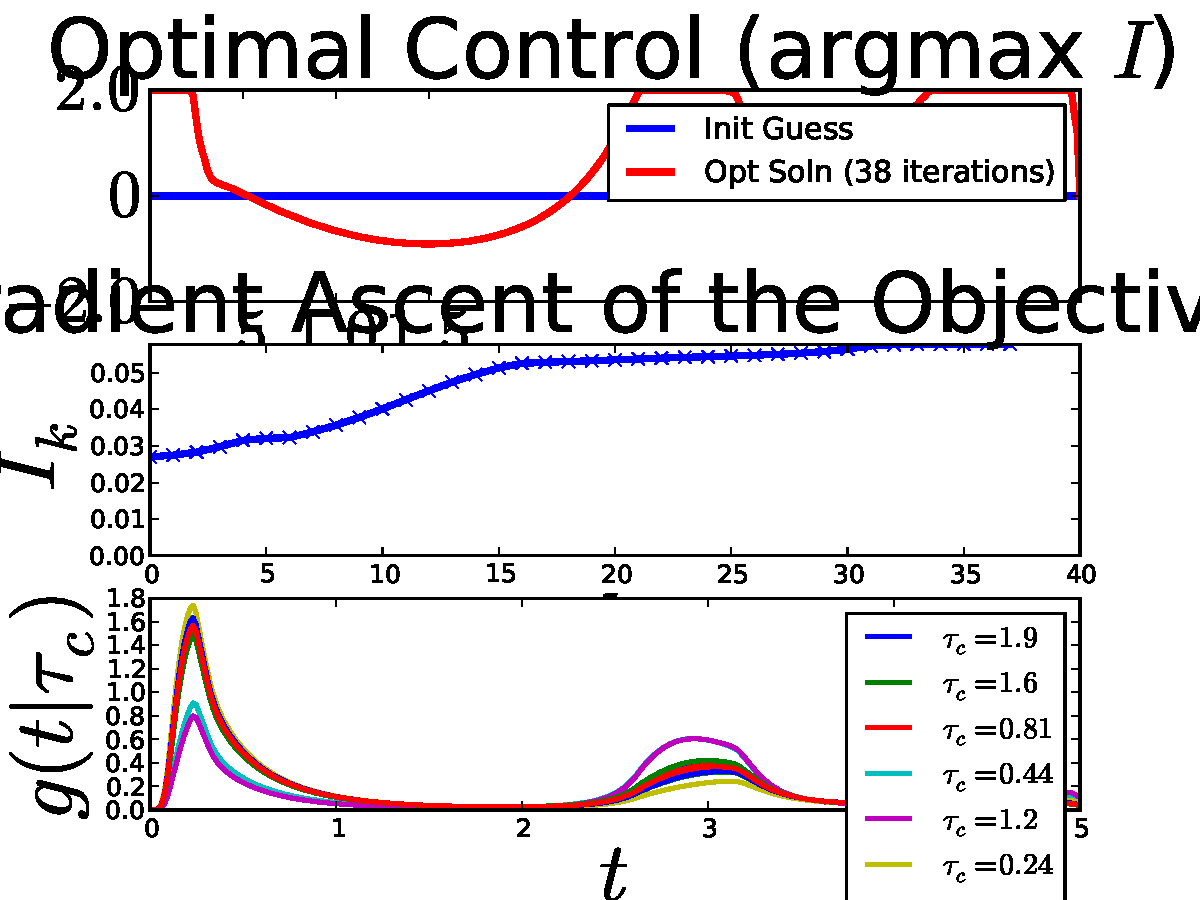
\includegraphics[width=0.48\textwidth]
{Figs/FP_Adjoint/PriorBox_wide_prior.pdf}
}
\subfloat[Tight Prior]
{
\label{fig:prior_spread_tight}
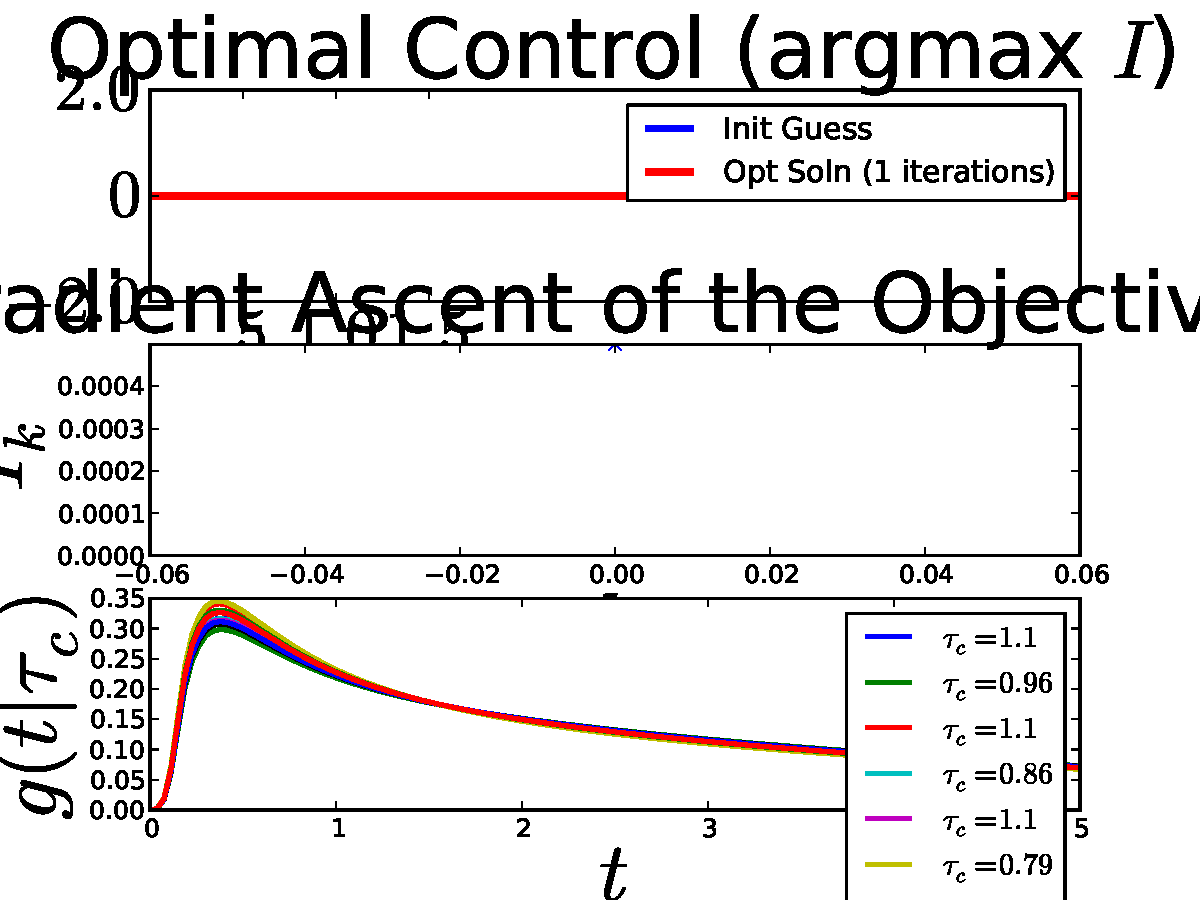
\includegraphics[width=0.48\textwidth]
{Figs/FP_Adjoint/PriorBox_concentrated_prior.pdf}
}
\caption[labelInTOC]{The effect of the spread (variance) of the prior on the
resulting optimal control}
\label{fig:prior_spread}
\end{center}
\end{figure}

Let's look at it another way, we will consider our basic prior as a function of
$w$
\begin{equation}
\rho(\tc) = 
\begin{cases}
	\tfrac 12 & \textrm{if } \tc= \in \{1- w, 1/(1-w) \}\\
	0   &\textrm{o/w }
\end{cases} 
\end{equation} 
and sweep for $w = .1:.1:.9$ (in matlab notation).

The results are in \cref{fig:effect_of_prior_width}. Looking at
\cref{fig:effect_of_prior_width}, we might be optimistic to hypothesize that we
should be doing this online and as the uncertainty (roughly speaking $w$) of the
parameter decreases, we should be changing the applied control\ldots This
brings us to {\sl adaptive } versions of our scheme which is NOT something we
have yet implemented. 
 
\begin{figure}[h]
\begin{center} 
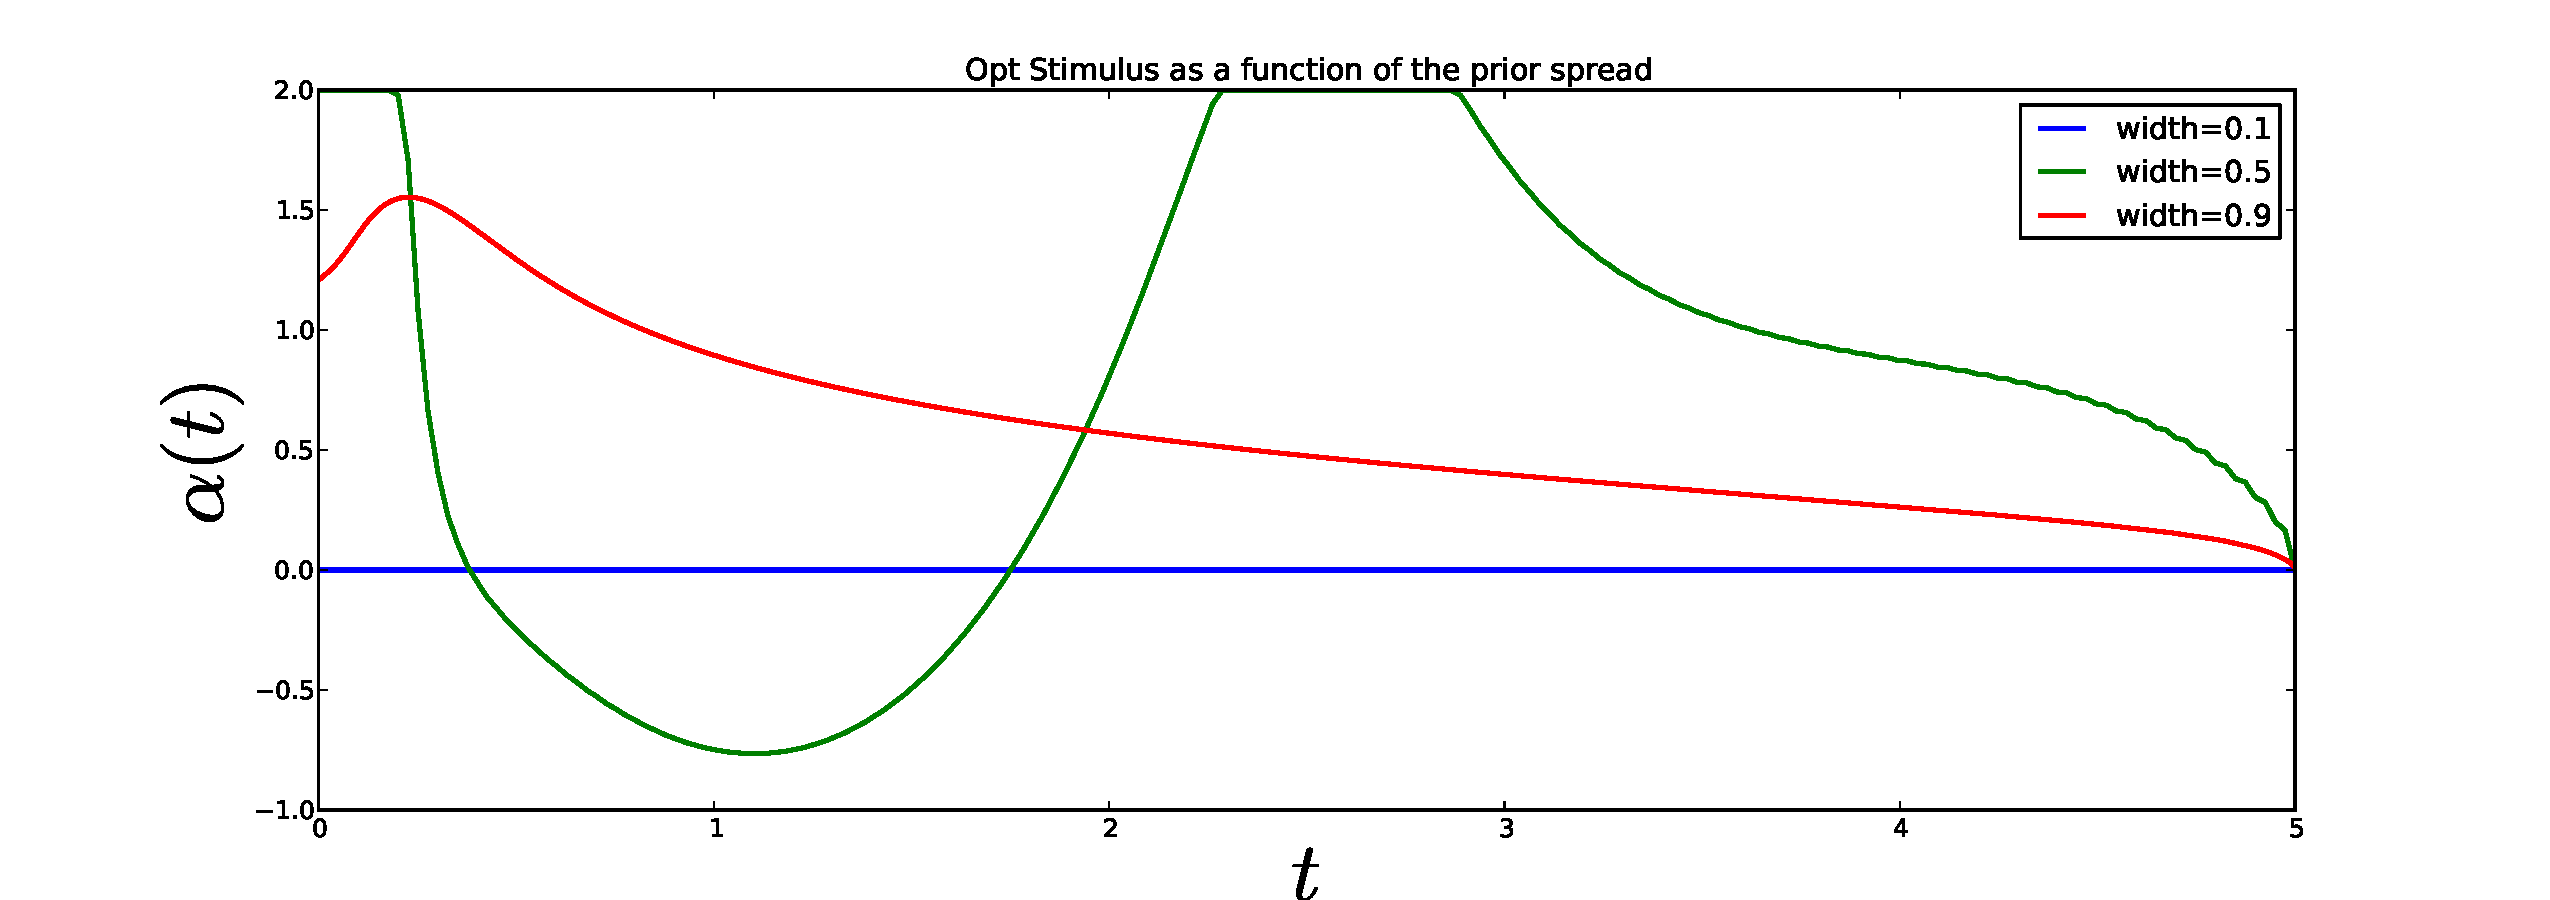
\includegraphics[width=\textwidth]
{Figs/FP_Adjoint/Effect_of_prior_spread.pdf} 
\caption[labelInTOC]{The effect of the width ($w$, a measure
of uncertainty) of the prior on the resulting optimal control}
\label{fig:effect_of_prior_width}
\end{center}
\end{figure}


\clearpage
\section{Basic Estimation Experiment}

We will run the following test:

Assume the true parameters $$
 \m = 0; \tc = 1; \b = 1.;
$$ We will assume we know $\b, \m$ and don't know the time constant, $\tc$ so we
are trying to maximize the Mutual Information between $\ts$ and $\tc$.
 
Let's assume a very simple uniform prior on $\tc$, $\tc_i = \{0.25, 1.5, 2.8
, 4.0\},$ each with probability 1/4.

Then running the gradient ascent (details of the gradient ascent are omitted) we
get the controls, objective and hitting time densities shown in 
\cref{fig:hitting_time_density_g_aopt_bprior}. The optimal control seems to be
independent of the number of point in the prior (i.e. instead of 4 we could use
32 pts with weight 1/32 and get the same opt. control as in
\cref{fig:hitting_time_density_g_aopt_bprior}). 

{\color{red} 
WARNING: The optimal control search routines is VERY sensitive to the initial
conditions. The one shown here is the one that has been empirically through
bitter experience been found to give the highest MI, but currently there is no
rigorous method to find it starting from arbitrary ICs (or from zero ICs for
that mater) }



\begin{figure}[htp]
\begin{center}
  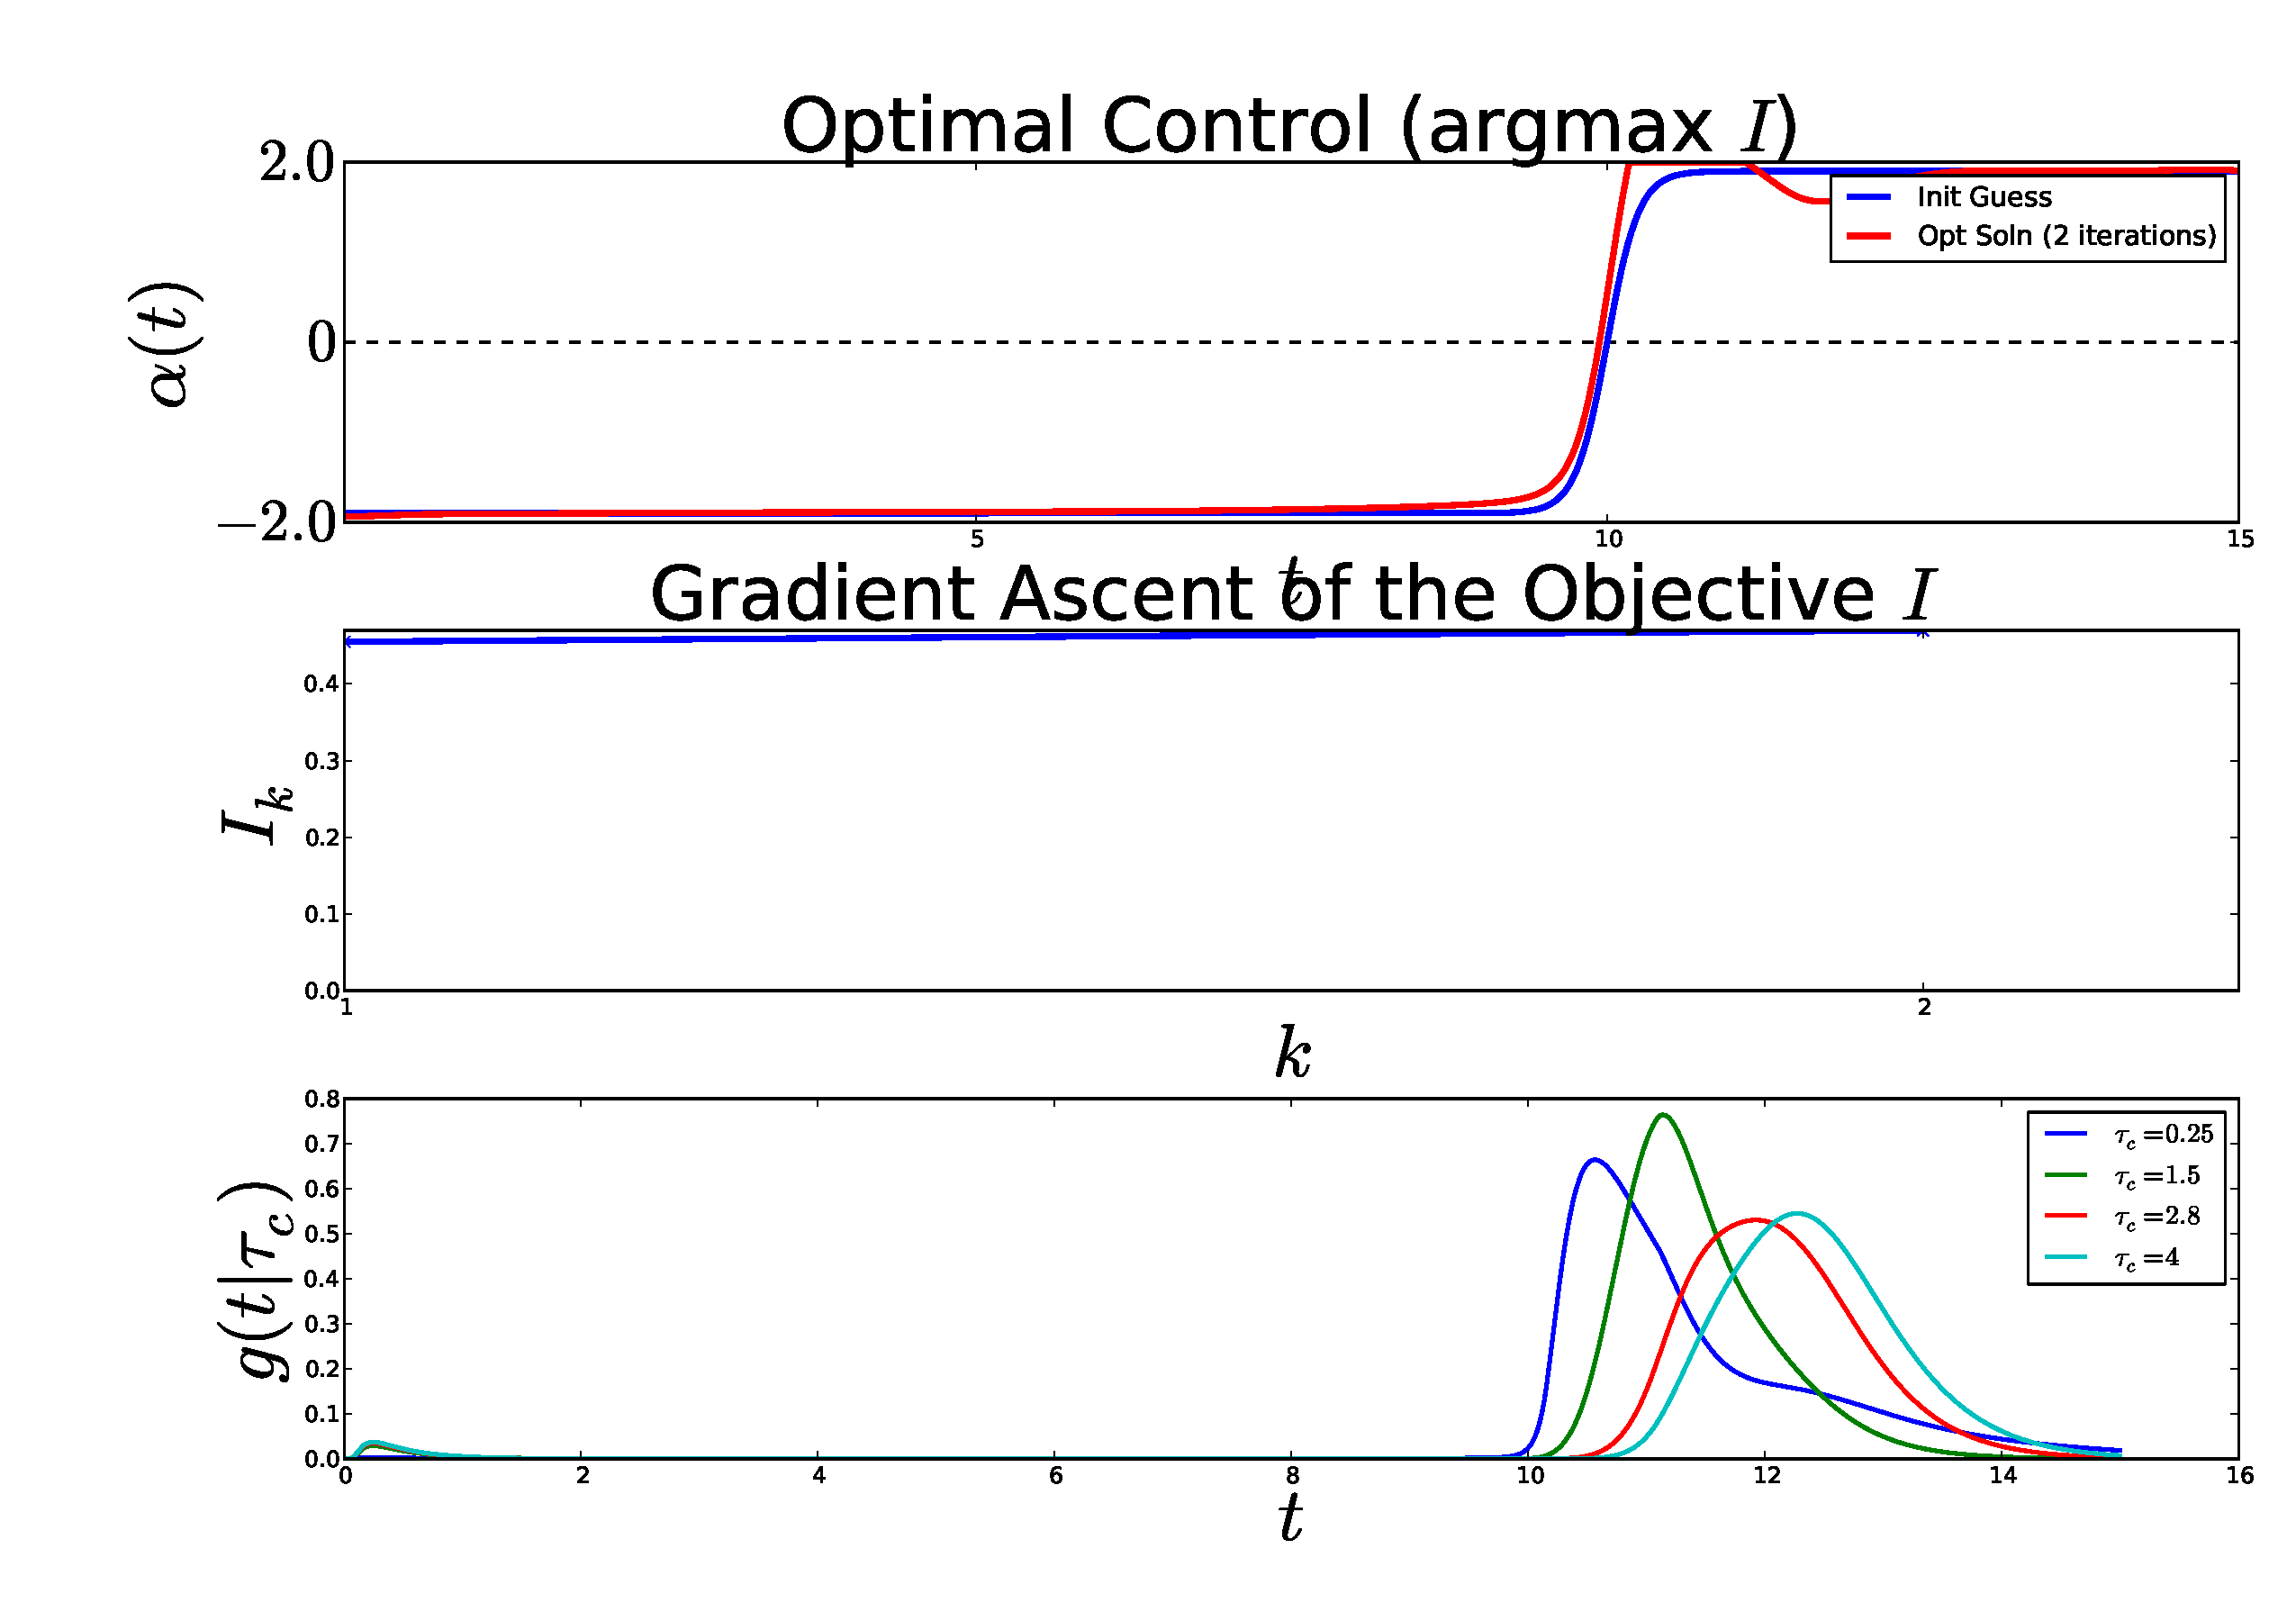
\includegraphics[width=1\textwidth]{Figs/FP_Adjoint/OptControl_MI_HT_4.pdf}
  \caption[labelInTOC]{The gradient ascent for the optimization of $I$ in
  \cref{eq:I_mutual_info_objective_in_terms_of_dixf}. Top panel, the initial and
  the optimal optimal controls, $\a_{0}(t), \a_{opt}(t)$. Middle Panel
  shows the progress of the Objective Mutual Information ($I$) 
  (\cref{eq:J_mutual_info_objective}). 
  The bottom plot shows the hitting times $g(t| \tc)$ corresponding to the 3
  distinct values of $\tc$ in the prior $\rho(\tc)$}  
  \label{fig:hitting_time_density_g_aopt_bprior}  
\end{center}   
\end{figure}  


\subsubsection{Switch point sweep}
At this point we suspect that the optimal solution is bang-bang, in the essense
of hold everything back and then excite maximally \ldots

We then sweep through the switch point $t_{switch}$ of exactly when the
bang-bang switch happens and see how it impacts the resulting objective, $I$.
The results are in \cref{fig:sweep_switchtime}. It seems that, at least for this
parameter set, there is quite an improvement in the objective by putting the switching
point past $t=6$, but going much beyond that there is no real difference. 

\begin{figure}[htp]
\begin{center}
  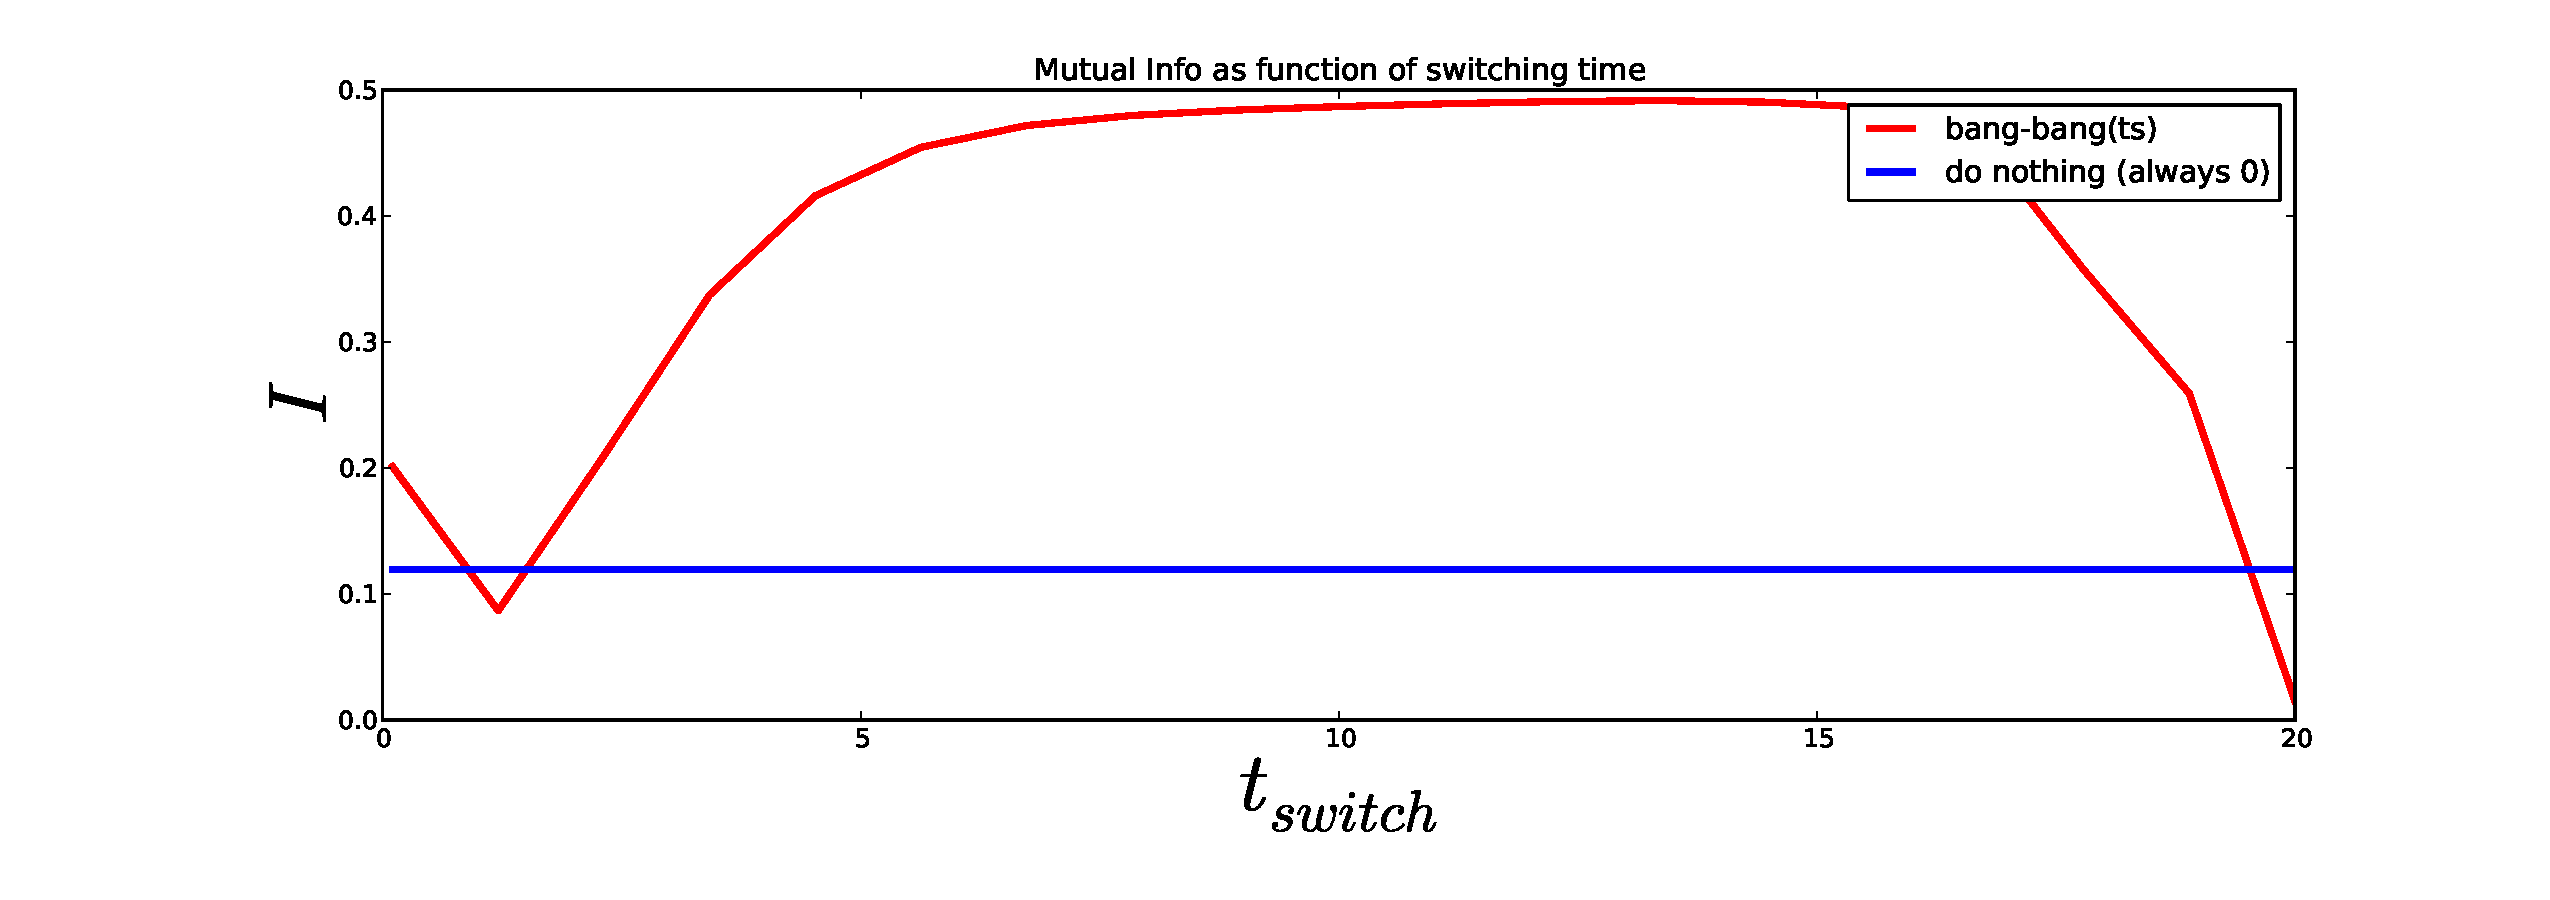
\includegraphics[width=1\textwidth]{/home/alex/Workspaces/Latex/OptEstimate/Figs/FP_Adjoint/SweepSwitchpoint.pdf}
  \caption[Effect of Switching time on Mutual Info Objective]{Effect of
  Switching time on Mutual Info Objective. Plotted is the objective, $I$, as a
  function of the switching time, $t_{switch}$, of a bang-bang switching control
  as in the top panel of \cref{fig:hitting_time_density_g_aopt_bprior}}
  \label{fig:sweep_switchtime}
\end{center}
\end{figure}

\subsubsection{Aside: the nitty-gritty of the estimation procedure}
We have posed a fairly-simple estimation objective, in that it amounts to single
variable optimization. The negative log-likelihood of an observed hitting-time
set $\{t_n\}$ is
\begin{equation}
l(\tc) = - \sum_n \log ( g(t_n | \tc) ) =  - \sum_n \log ( -D \di_x f(t_n |
\tc) |_{\xth} )
\end{equation}

The distributions are exemplified in
\cref{fig:log_likelihood_beta_examples_100000},
for three different values of $N_s =  1e5$. We see that for the constant
stimulations, $\a = \a_{crit}, \a_{max}$ it is very hard to
distinguish between different values of $\tc$. 

In \cref{fig:log_likelihood_beta_examples_100000} as well as in 
\cref{fig:hitting_time_density_g_aopt_bprior}, we get an indication for why
the 'optimal control' is better than the constants. For the constant control
the different hitting time densities look like local perturbations of each
other, either a little more or a little less, but for the optimal control they
are shifted, which means that we see the first indications that the Opt Control,
might have some superiority over the 'Crit' Control (for example) as it seems to estimate a $\tc$ closer to 1 (the 'true' value). However, on average, the different shapes of $\a(t)$ seems to have a very limited impact on the estimates for $\tc$ (even though it has a very obvious impact on the shape of the hitting time distribution $g(t)$).

\begin{figure}[h] 
\begin{center}
\subfloat[opt]
{
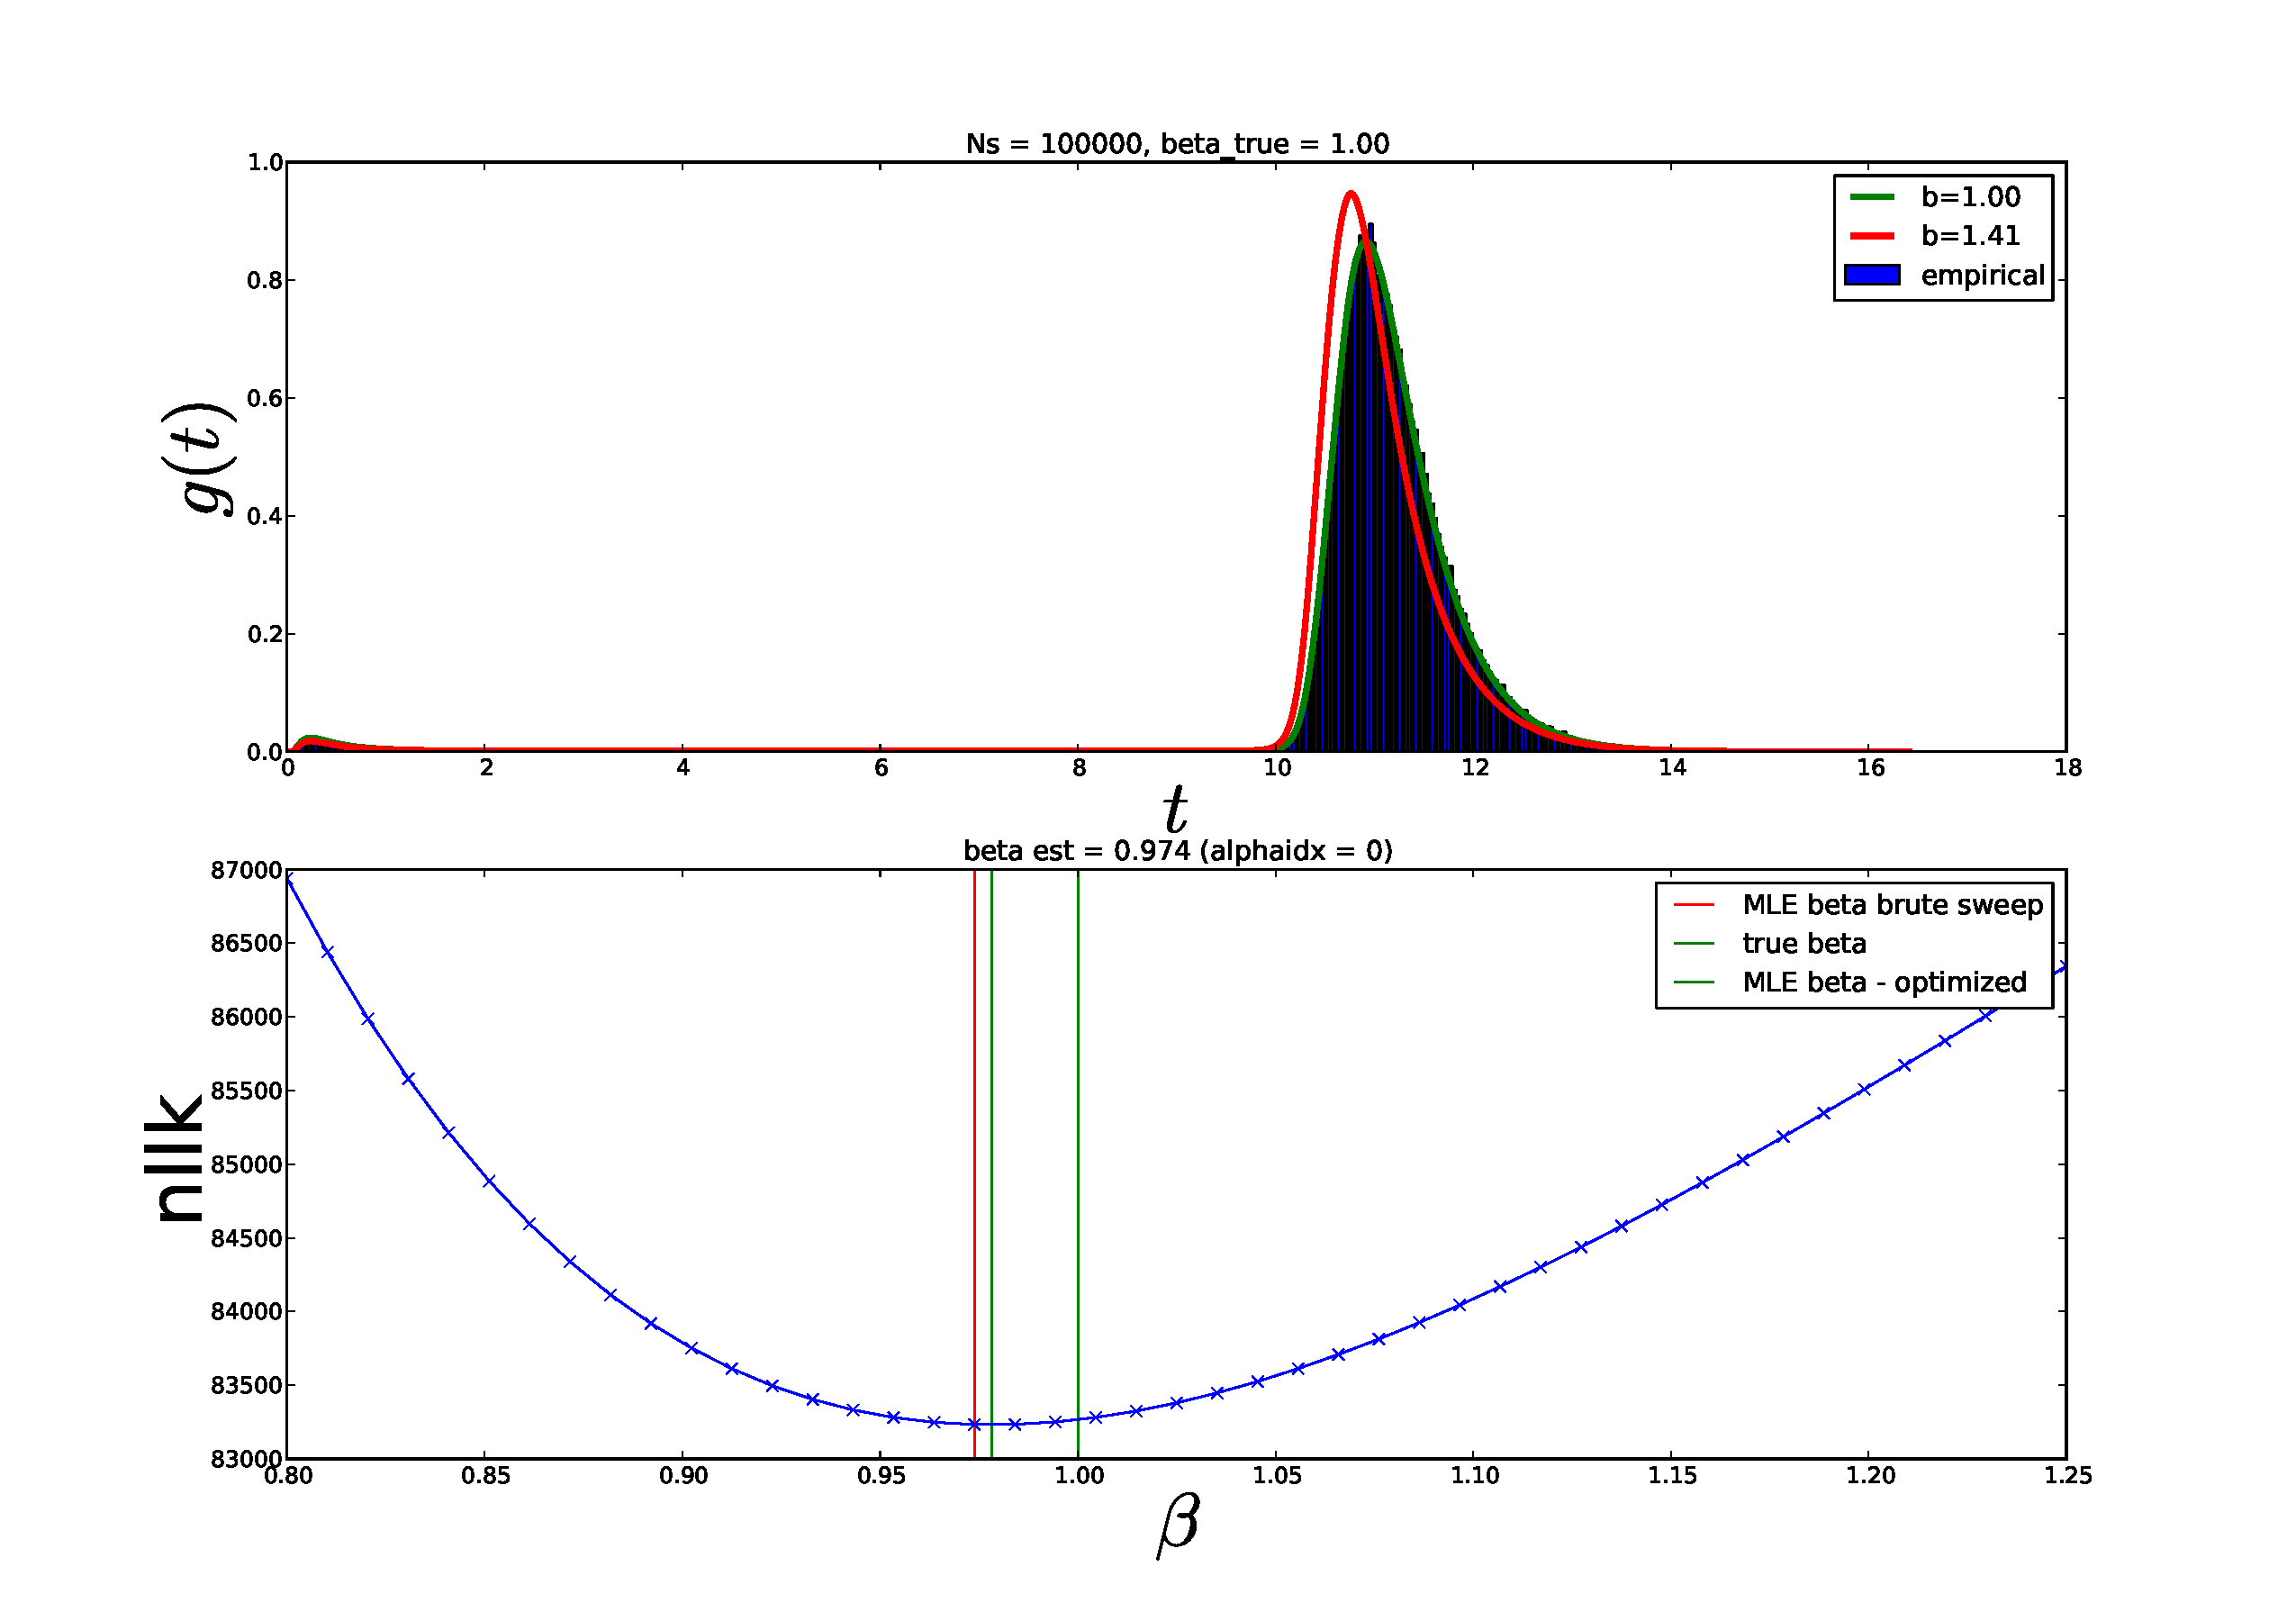
\includegraphics[width=.75\textwidth]
{Figs/HitTime_MI_TauChar_Adjoint_Estimate/Adjoint_TauChar_Estimator_estimatorWorkbench_b=0x100000_a0.pdf}
}
\\
\subfloat[crit] 
{
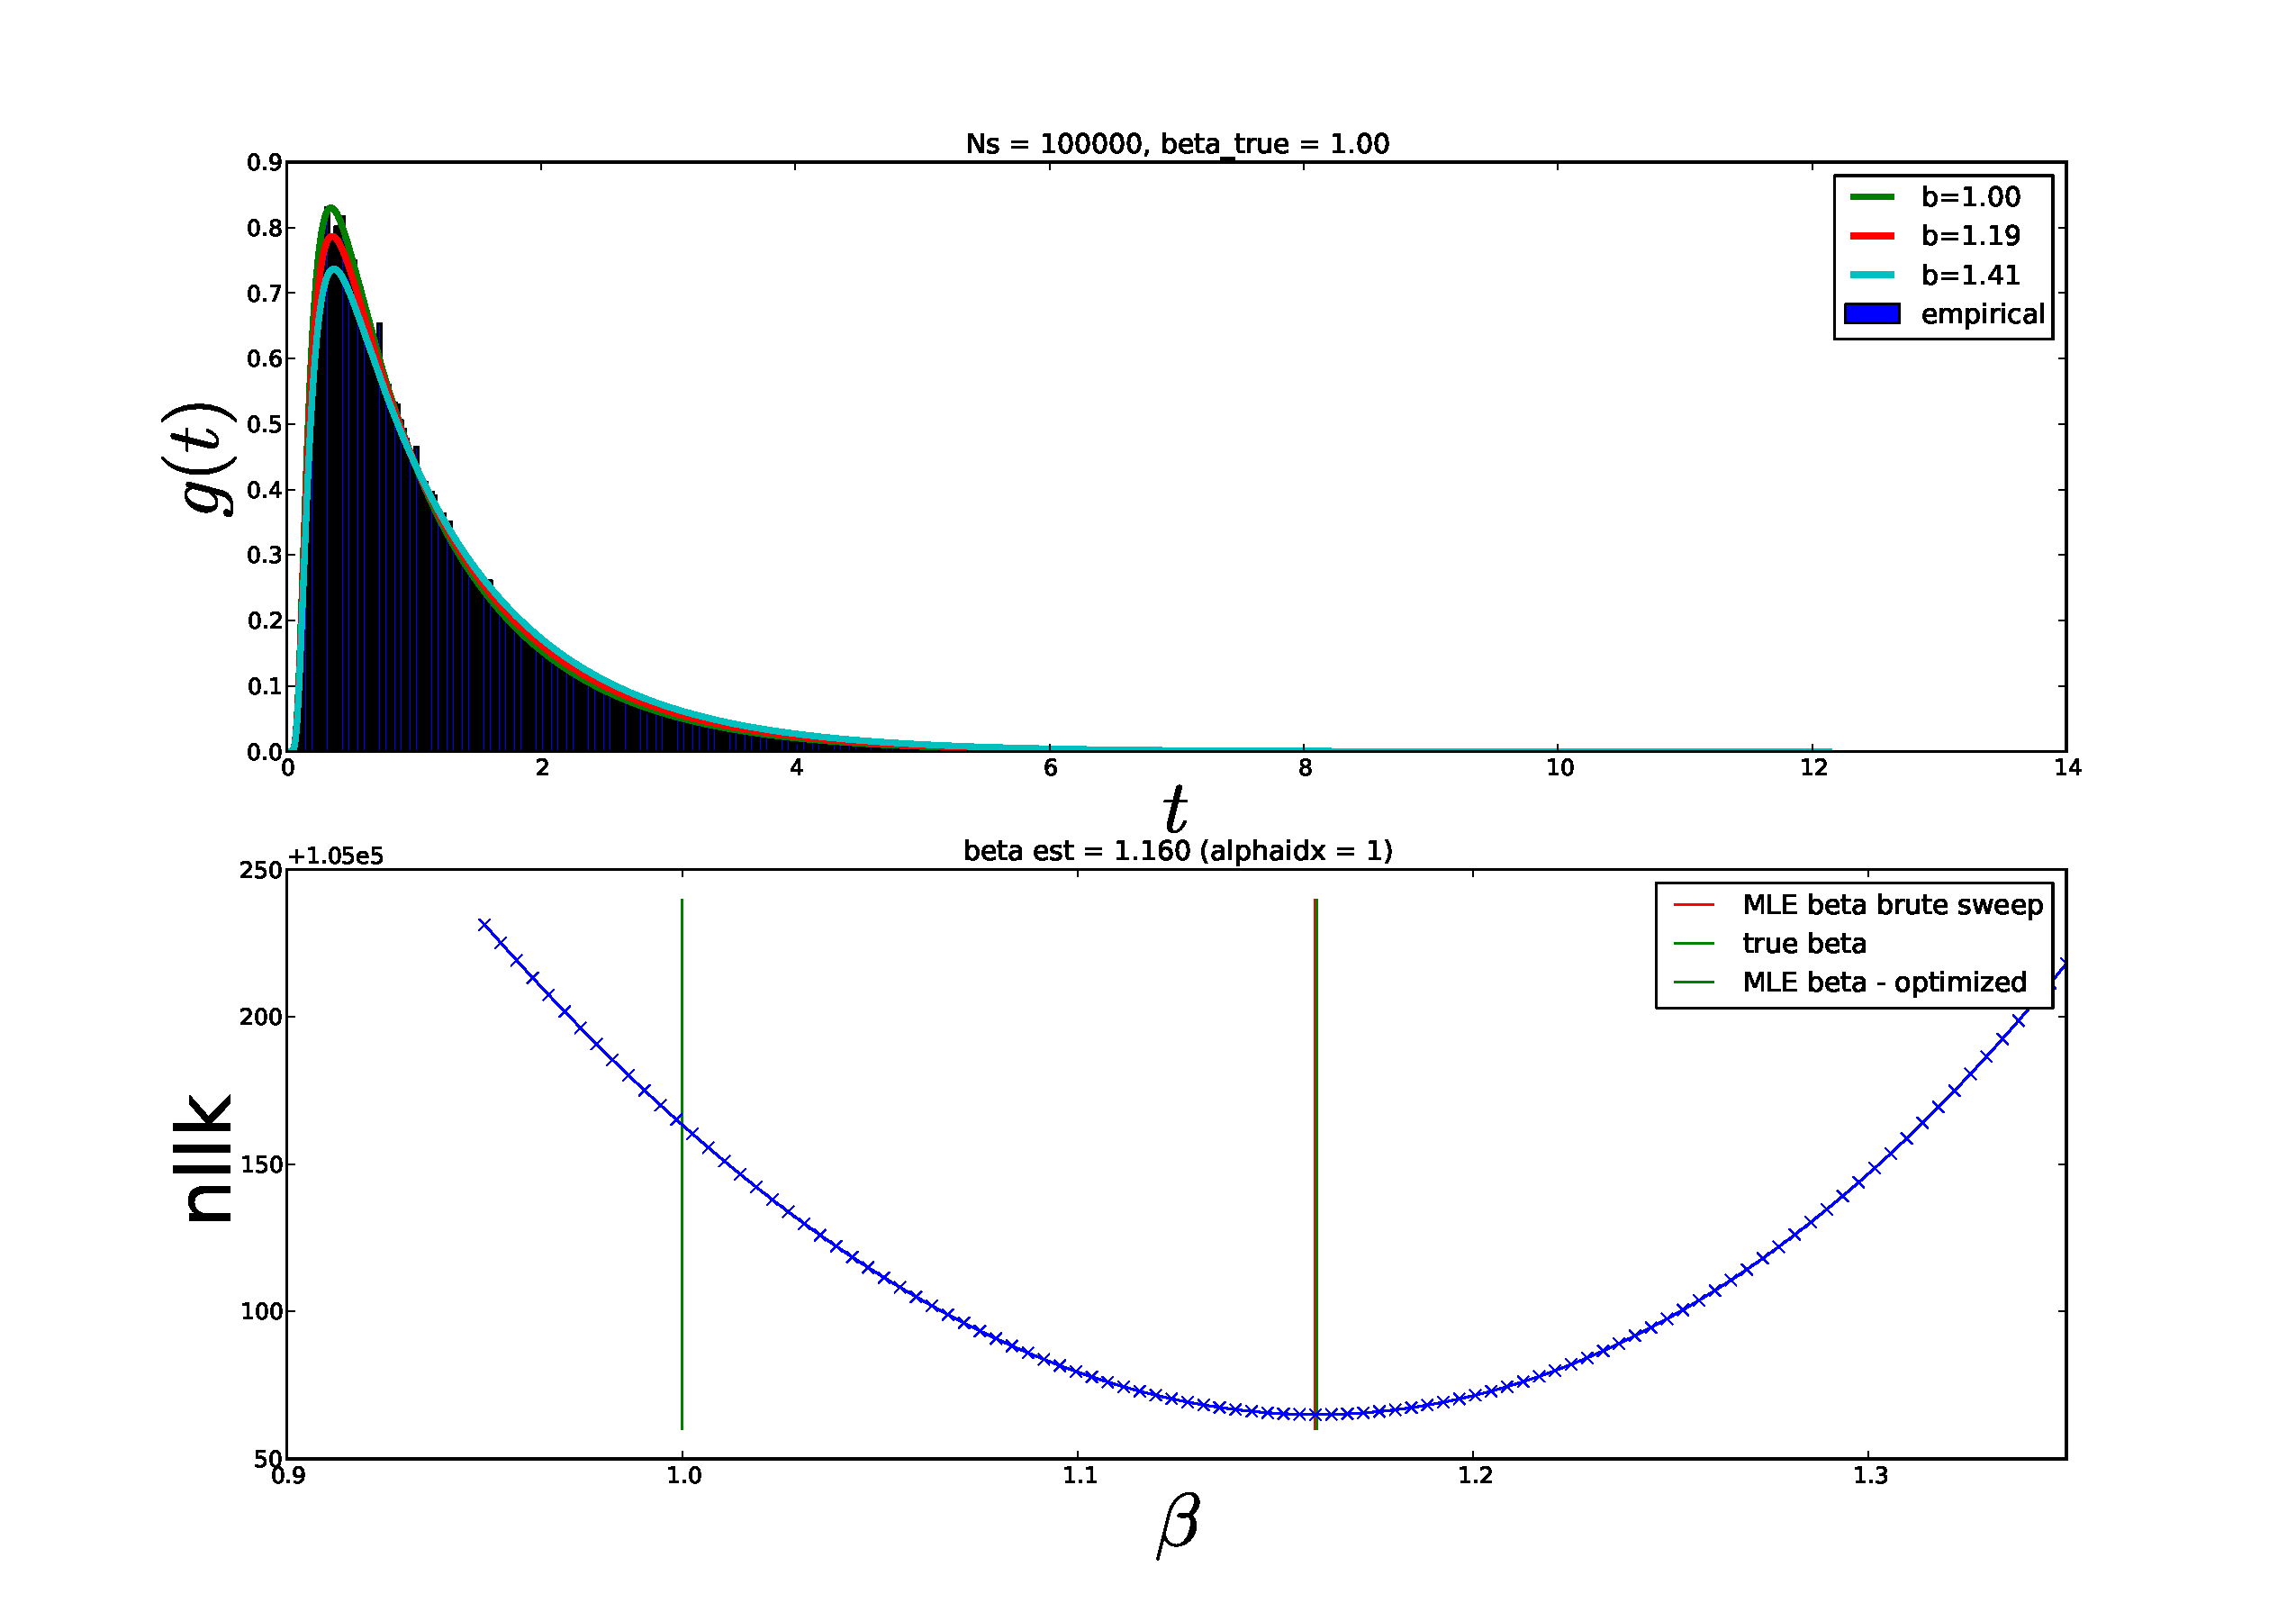
\includegraphics[width=.75\textwidth]
{Figs/HitTime_MI_TauChar_Adjoint_Estimate/Adjoint_TauChar_Estimator_estimatorWorkbench_b=0x100000_a1.pdf}
}
\\
\subfloat[max]
{
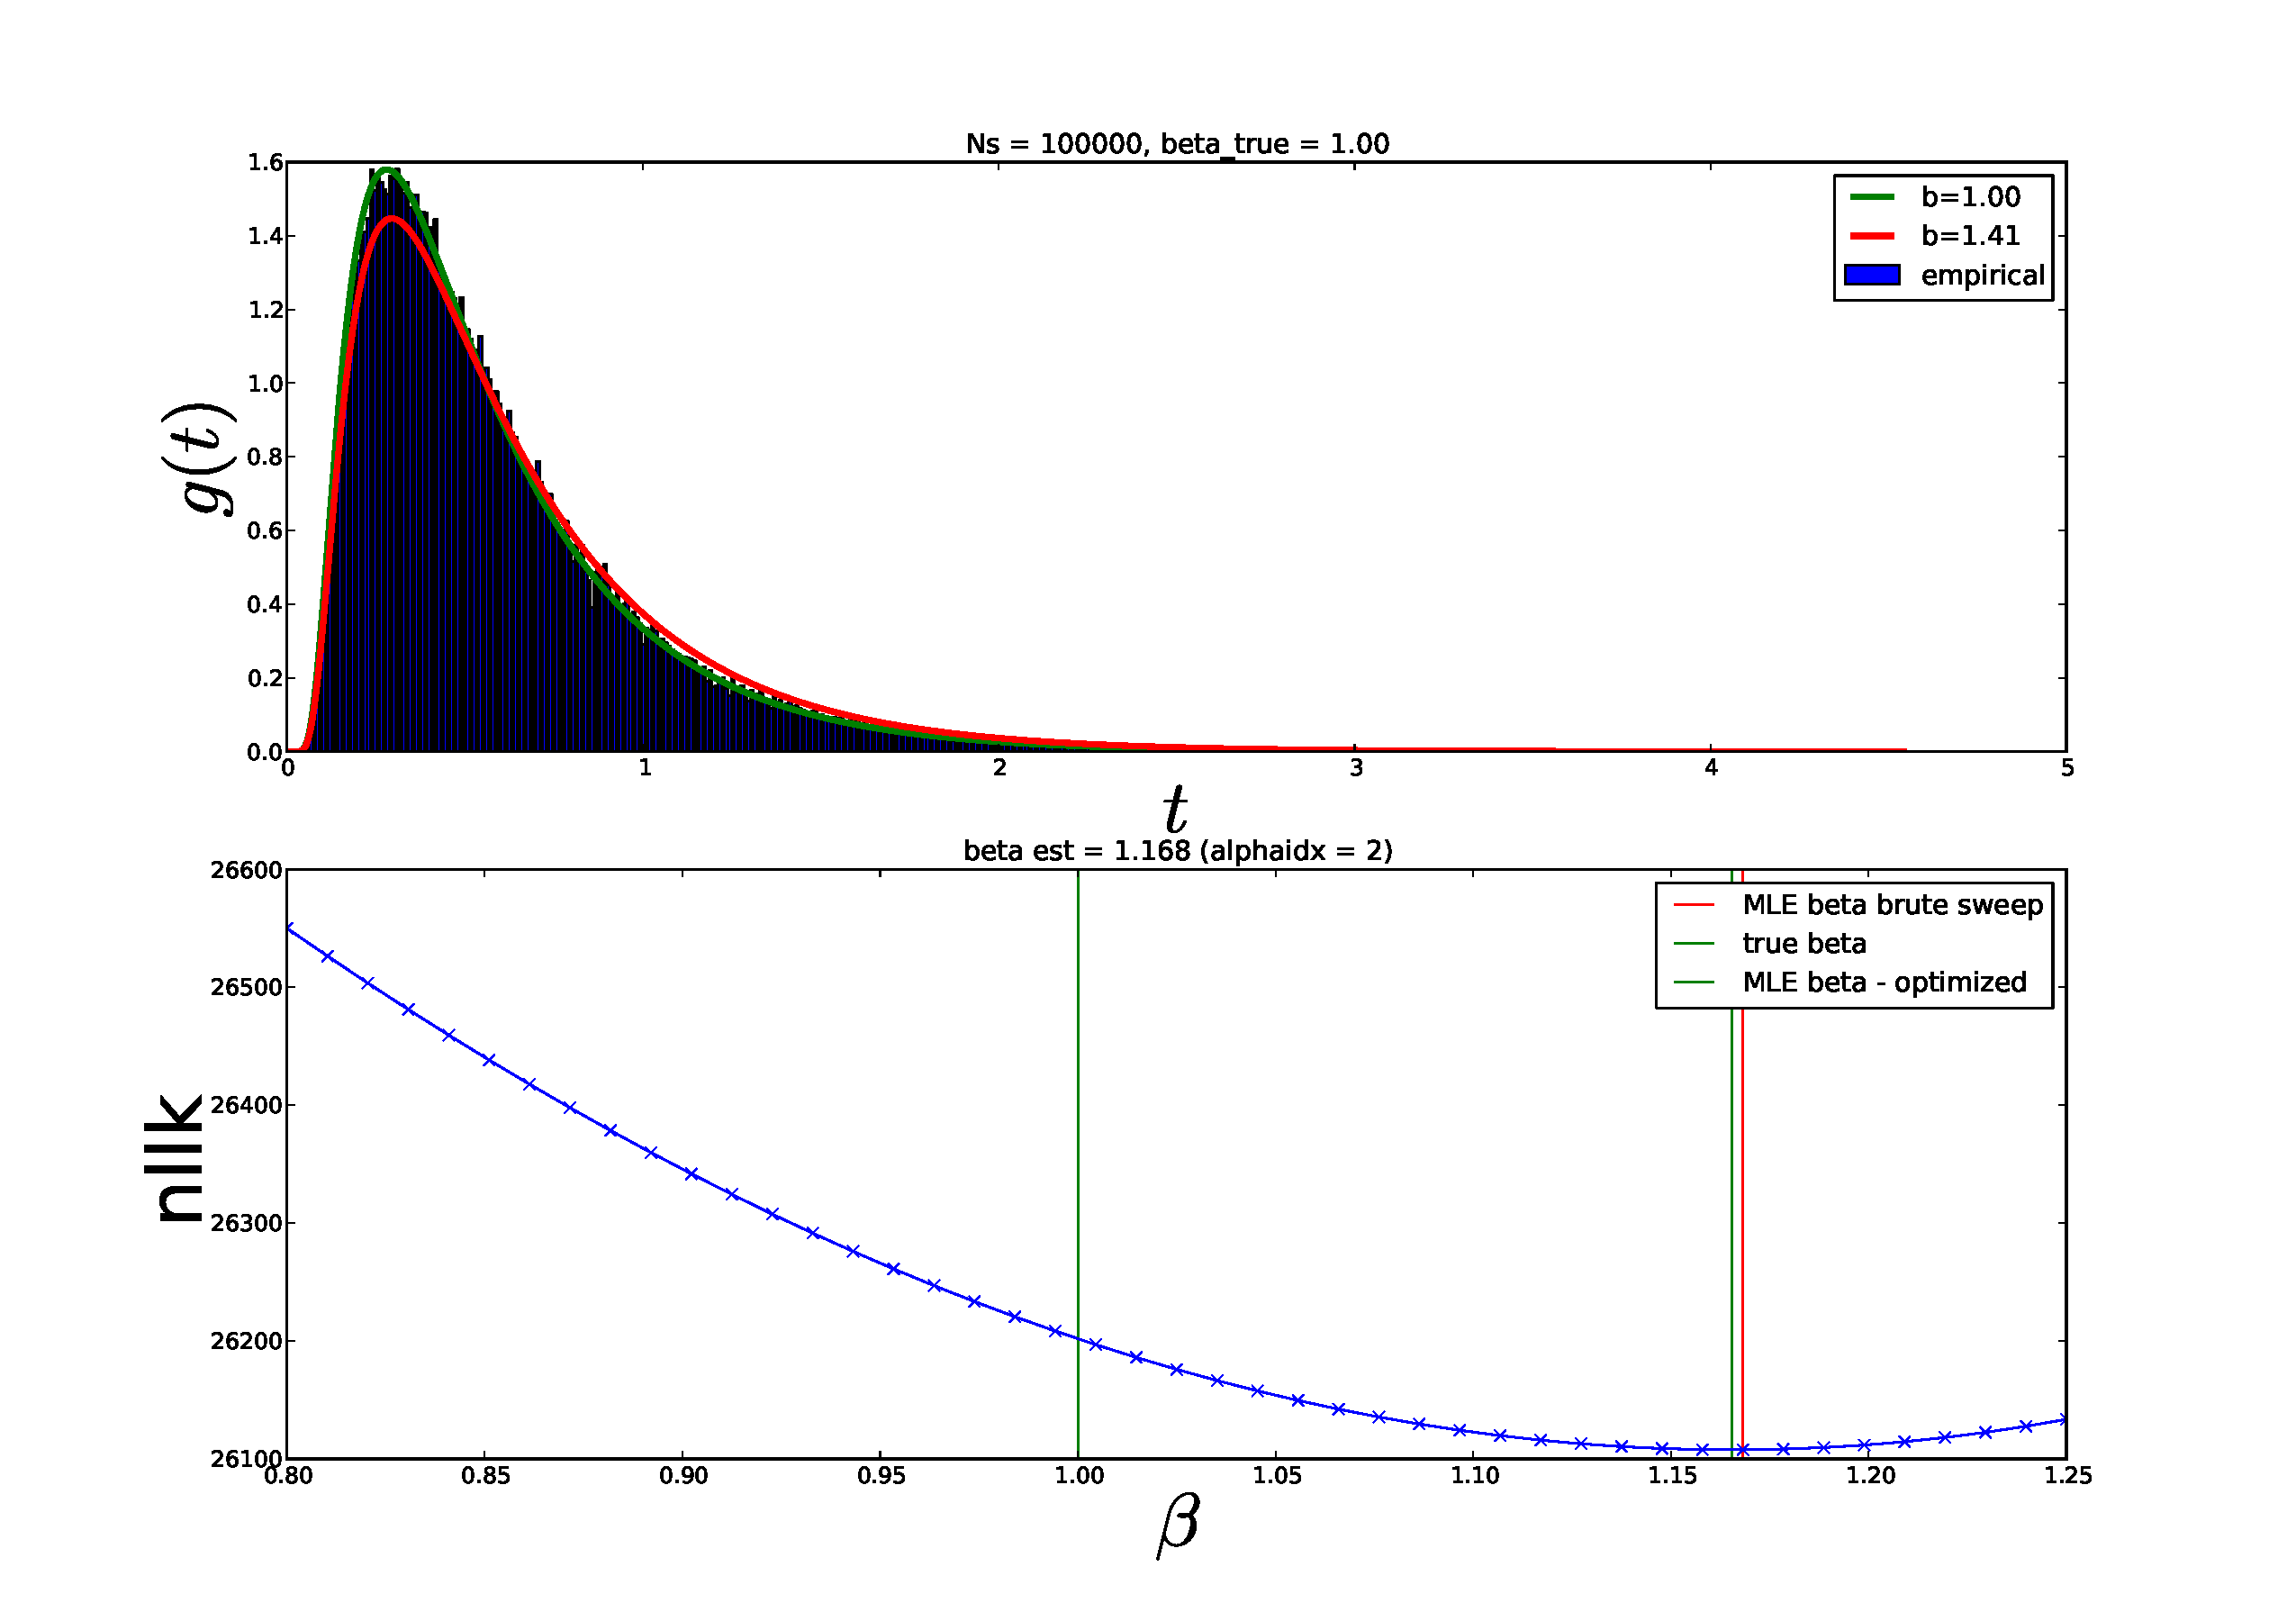
\includegraphics[width=.75\textwidth]
{Figs/HitTime_MI_TauChar_Adjoint_Estimate/Adjoint_TauChar_Estimator_estimatorWorkbench_b=0x100000_a2.pdf}
}
\caption[labelInTOC]{Example of Empirical vs.\ Analytical Hitting time
distributions, $g(t|\t;\a)$, and the associated log-likelihoods. $N_s = 1e5$
hits}
\label{fig:log_likelihood_beta_examples_100000}
\end{center}
\end{figure}  

\clearpage



\subsection{Batch Performance of the perturbations over the estimators.}
As is we have 3 candidates for perturbing the hitting times: 
\begin{enumerate}
  \item 
the optimal gradient-ascent-based  control $\a_{opt}$ (see
\cref{fig:hitting_time_density_g_aopt_bprior} top panel)
\item   the 'critical' constant control
$\a_{crit}$, ($\a_{crit}(t) =  \tc$)
\item  the max constant control, $\amax$ ($=2$)
\end{enumerate} 

We now simulate $N_b $ blocks of $N_s $ hitting times each for the
3 alphas and then estimate $\tc$ over each set using MaxLikelihood over our
computed expression for the density, $g(t|\tc; \a(t) )$). 
Naturally, for each control, we use the same Gaussian random draws per block of
$N_s$ Hitting of times). See \cref{fig:log_likelihood_beta_examples_100000} for
a empirical distribution of $\ts$ for $N_s = 1e5$
%\usepackage{graphics} is needed for \includegraphics
% \begin{figure}[htp]
% \begin{center}
%   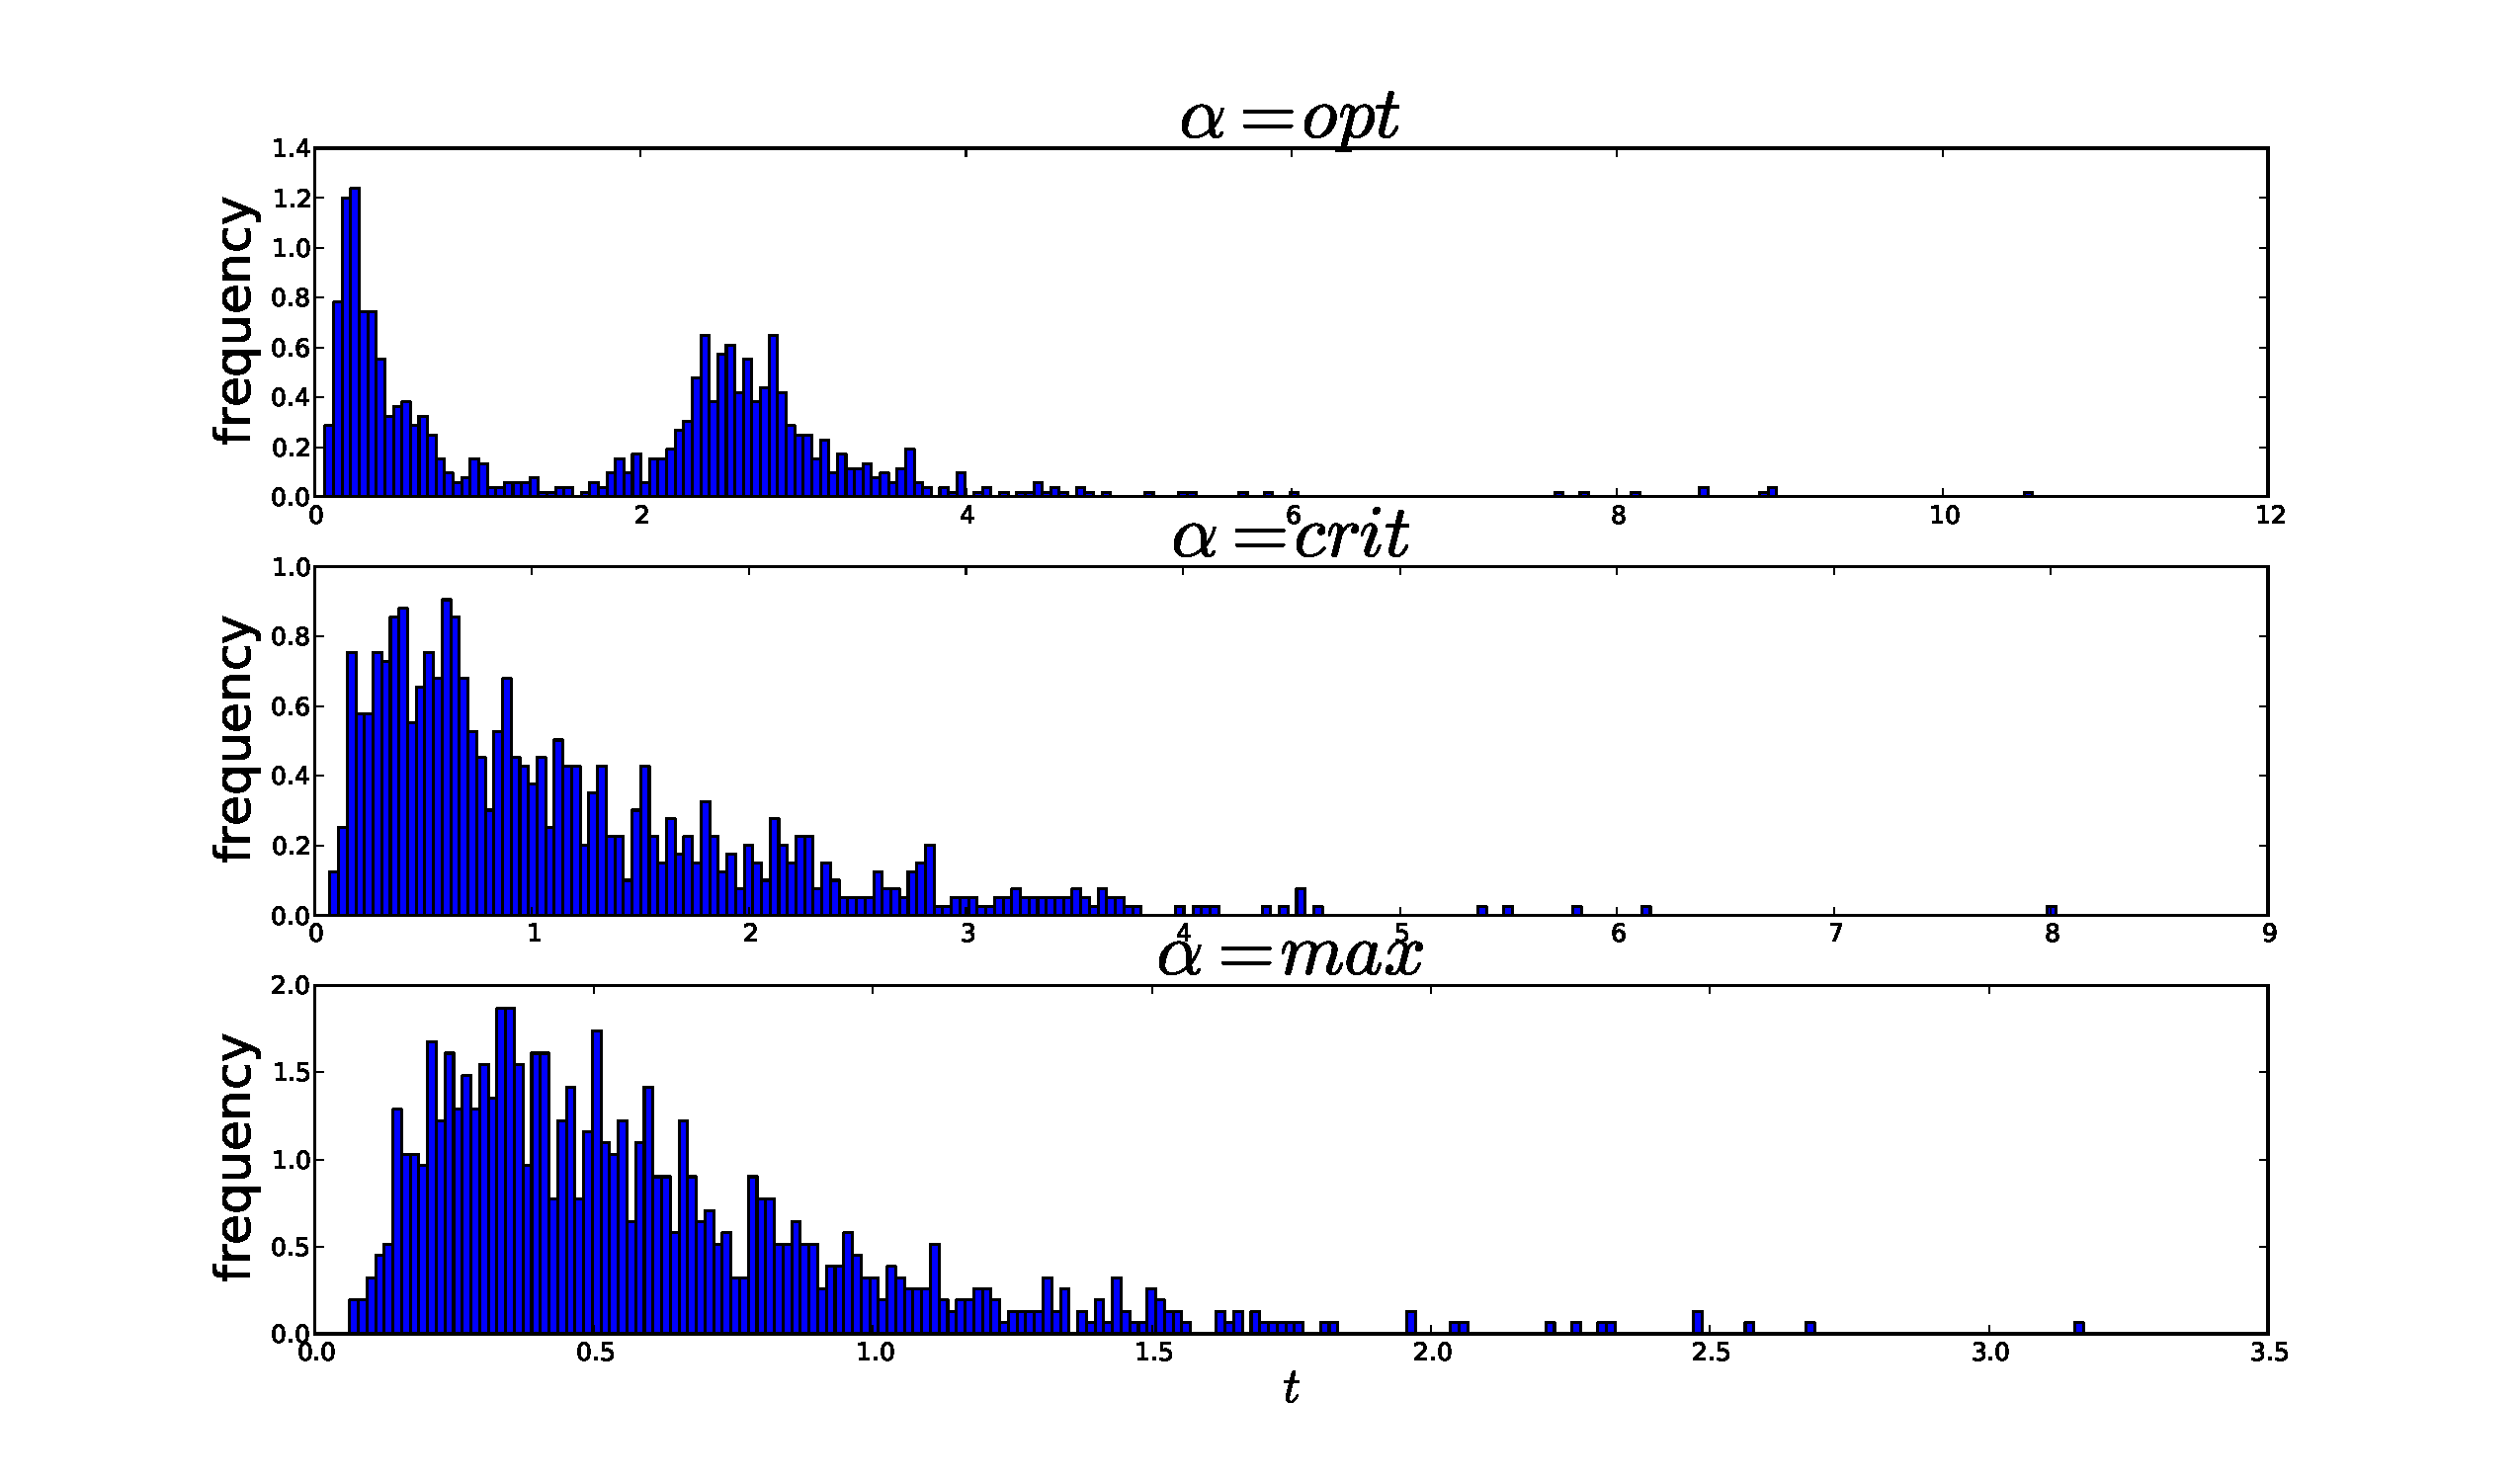
\includegraphics[width=\textwidth]{Figs/HitTime_MI_TauChar_Adjoint_Estimate/three_pt_prior_thits_distn.pdf}
%   \caption[labelInTOC]{Empirical Hitting-TIme distributions for the different
%   choices of $\a$}
%   \label{fig:empirical_hitting_times_3alphas}
% \end{center}
% \end{figure}

The estimation results are tabulated in in
\cref{tab:beta_estimates_from_hitting_times_different_alphas}.

\begin{table}
\subfloat[$N_b=1000, N_s = 1e2$]{
\begin{tabular}{ccc}
\input{Figs/HitTime_MI_TauChar_Adjoint_Estimate/tauchar_hit_time_100.txt}
\end{tabular}
}
\subfloat[$N_b=100, N_s = 1e3$]{
\begin{tabular}{ccc}
\input{Figs/HitTime_MI_TauChar_Adjoint_Estimate/tauchar_hit_time_1000.txt}
\end{tabular}
}\\
\subfloat[$N_b=10, N_s = 1e4$]{
\begin{tabular}{ccc}
\input{Figs/HitTime_MI_TauChar_Adjoint_Estimate/tauchar_hit_time_10000.txt}
\end{tabular}
} 
\subfloat[$N_b=1, N_s = 1e5$]{
\begin{tabular}{ccc}
\input{Figs/HitTime_MI_TauChar_Adjoint_Estimate/tauchar_hit_time_100000.txt}
\end{tabular}
}
\caption[Static $\tau$ MLE estimates]{Results for the estimates arising from
simulations using various values of $\a$ (opt, crit, max). In each sub-table there are $N_b$
parameter estimates for each distinct $\a$, with $N_s$ hitting times used to
form an $\tc-$estimate.  The 'true' value of $\tc$ is $\tc=1$, i.e. $\log(\tc)
= 0$. Also see \cref{fig:beta_estimates_from_hitting_times_different_alphas}}
\label{tab:beta_estimates_from_hitting_times_different_alphas} 
\end{table}   

\begin{figure}[h]
\begin{center}
\subfloat[$N_b=1e3, N_s = 1e2$]
{
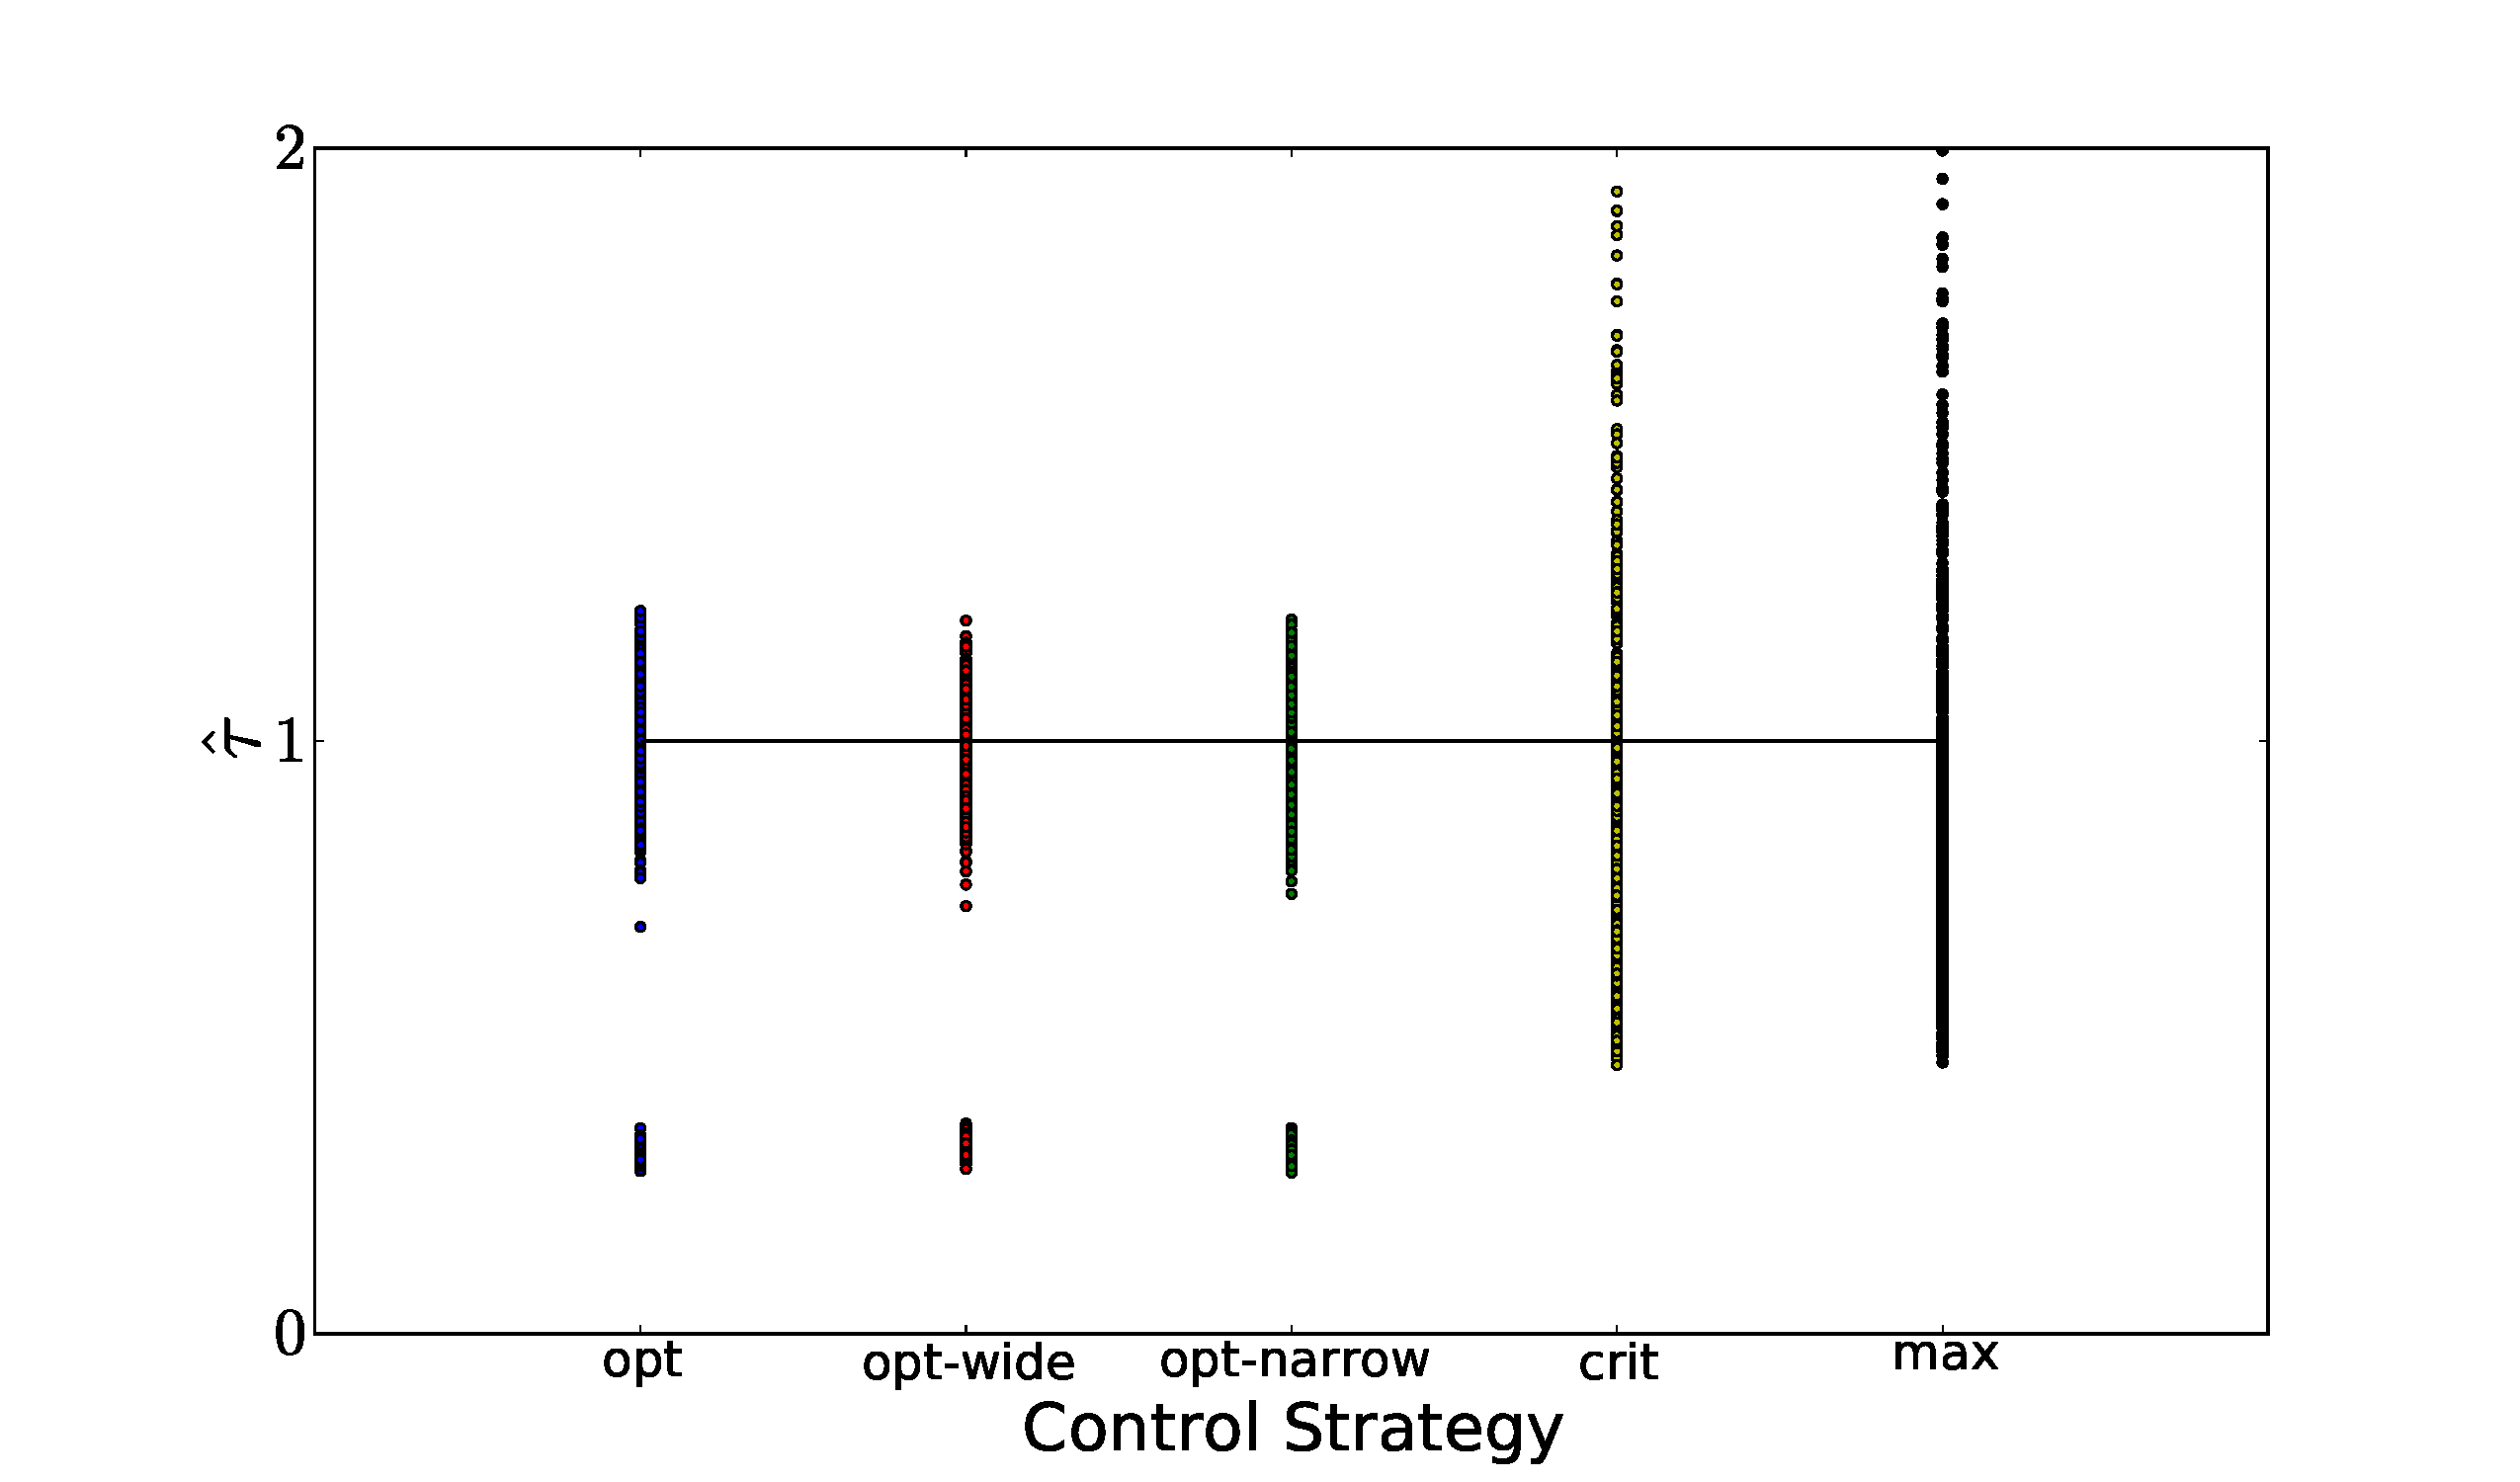
\includegraphics[width=0.48\textwidth]
{Figs/HitTime_MI_TauChar_Adjoint_Estimate/miestimates_scatterplot_Nb1000_Ns100.pdf}
}
\subfloat[$N_b=1e3, N_s = 1e2$]
{
\label{fig:label2}
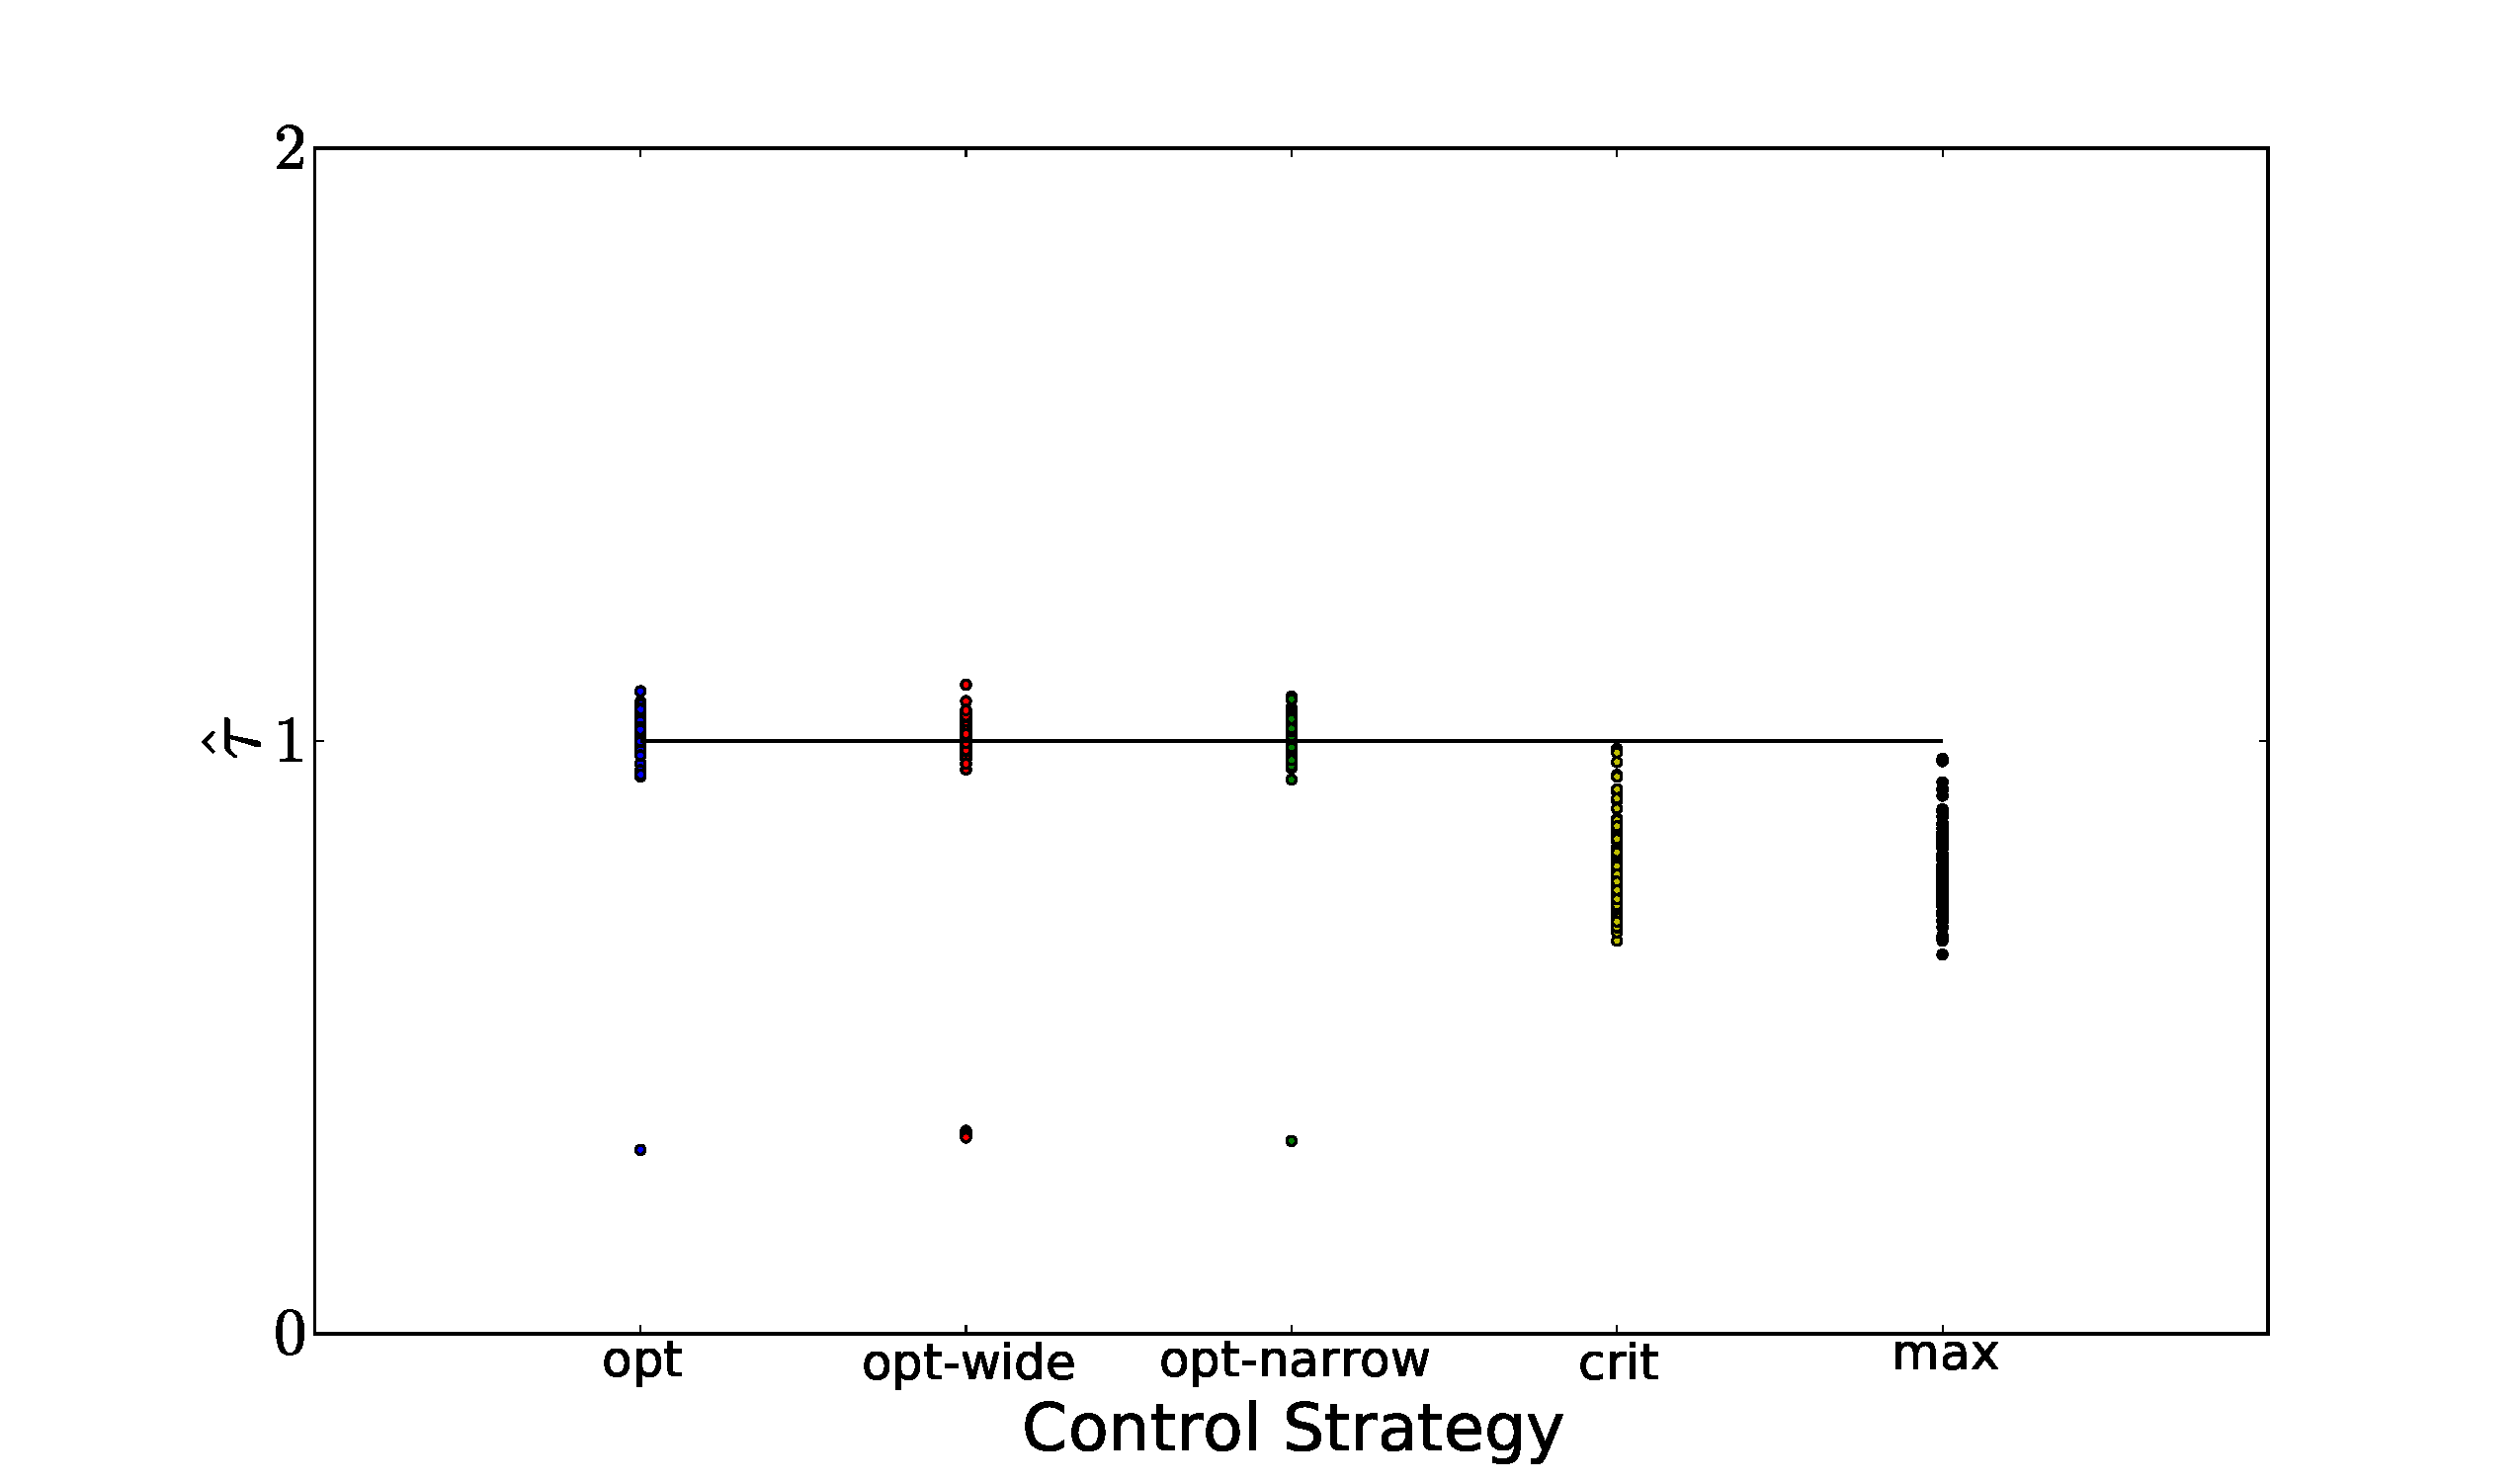
\includegraphics[width=0.48\textwidth]
{Figs/HitTime_MI_TauChar_Adjoint_Estimate/miestimates_scatterplot_Nb100_Ns1000.pdf}
}
\\
\subfloat[$N_b=1e1, N_s = 1e4$]
{
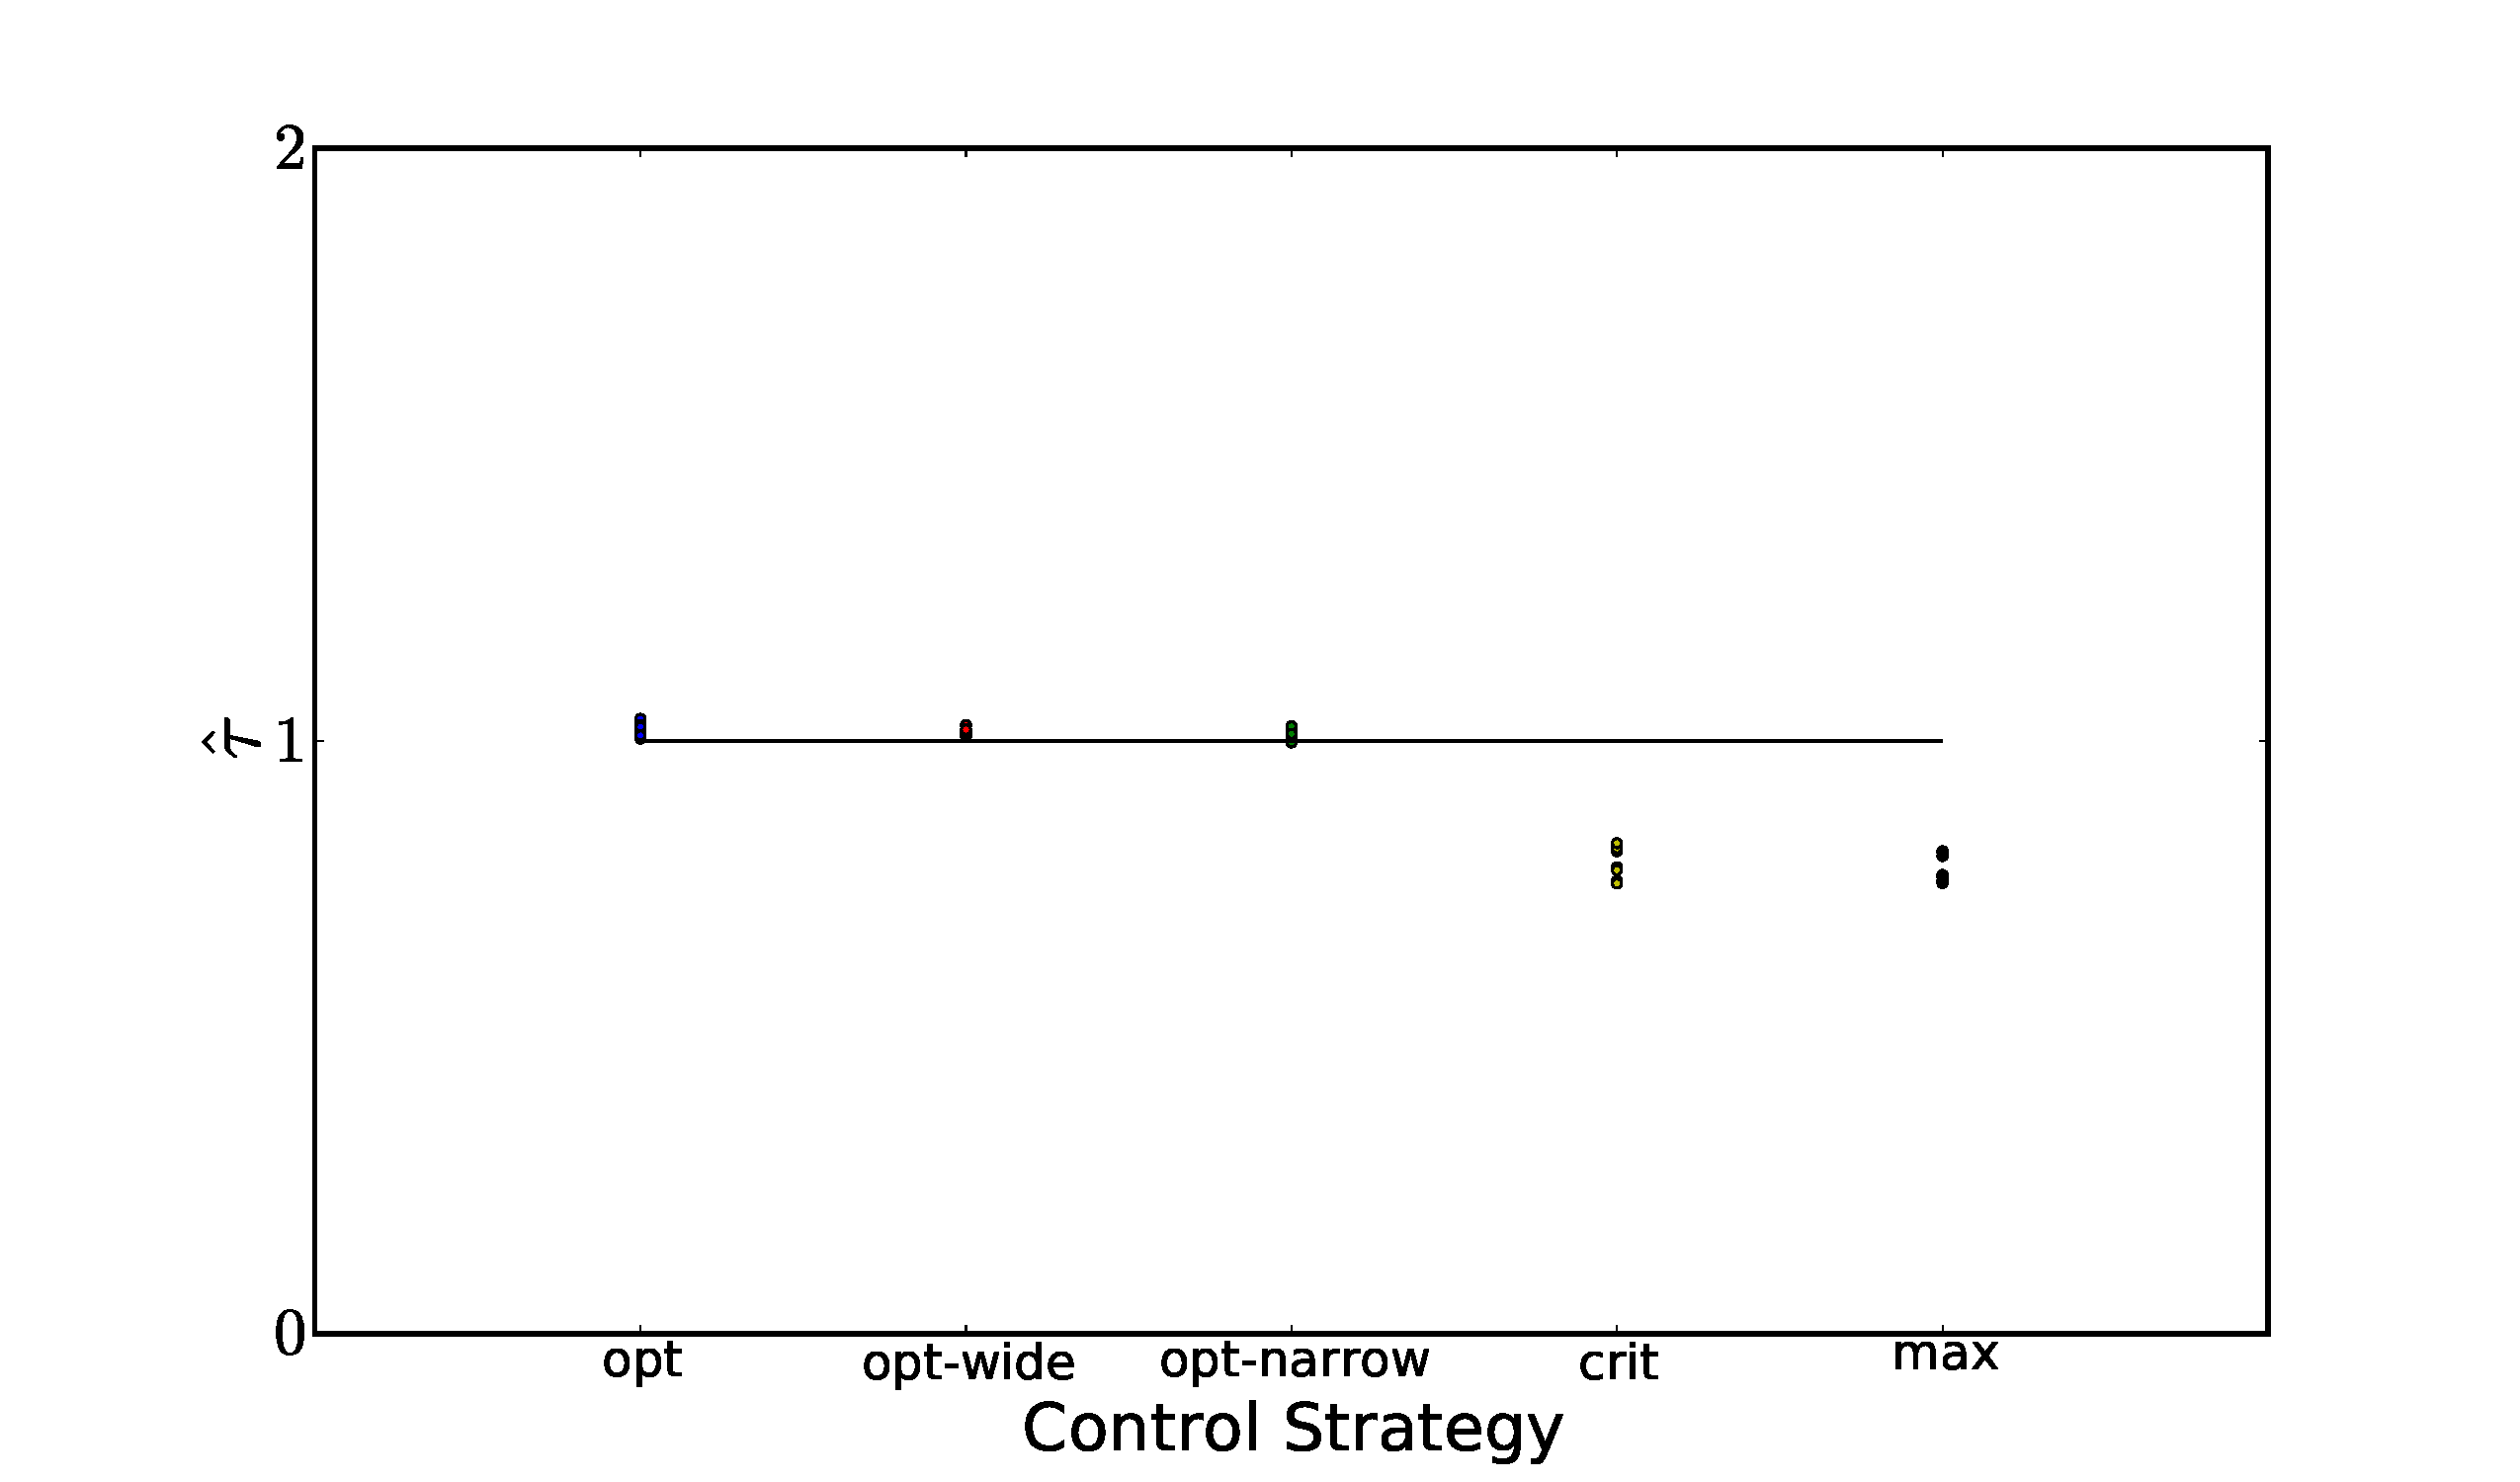
\includegraphics[width=0.48\textwidth]
{Figs/HitTime_MI_TauChar_Adjoint_Estimate/miestimates_scatterplot_Nb10_Ns10000.pdf}
}
\subfloat[$N_b=1e1, N_s = 1e5$]
{
\label{fig:label2}
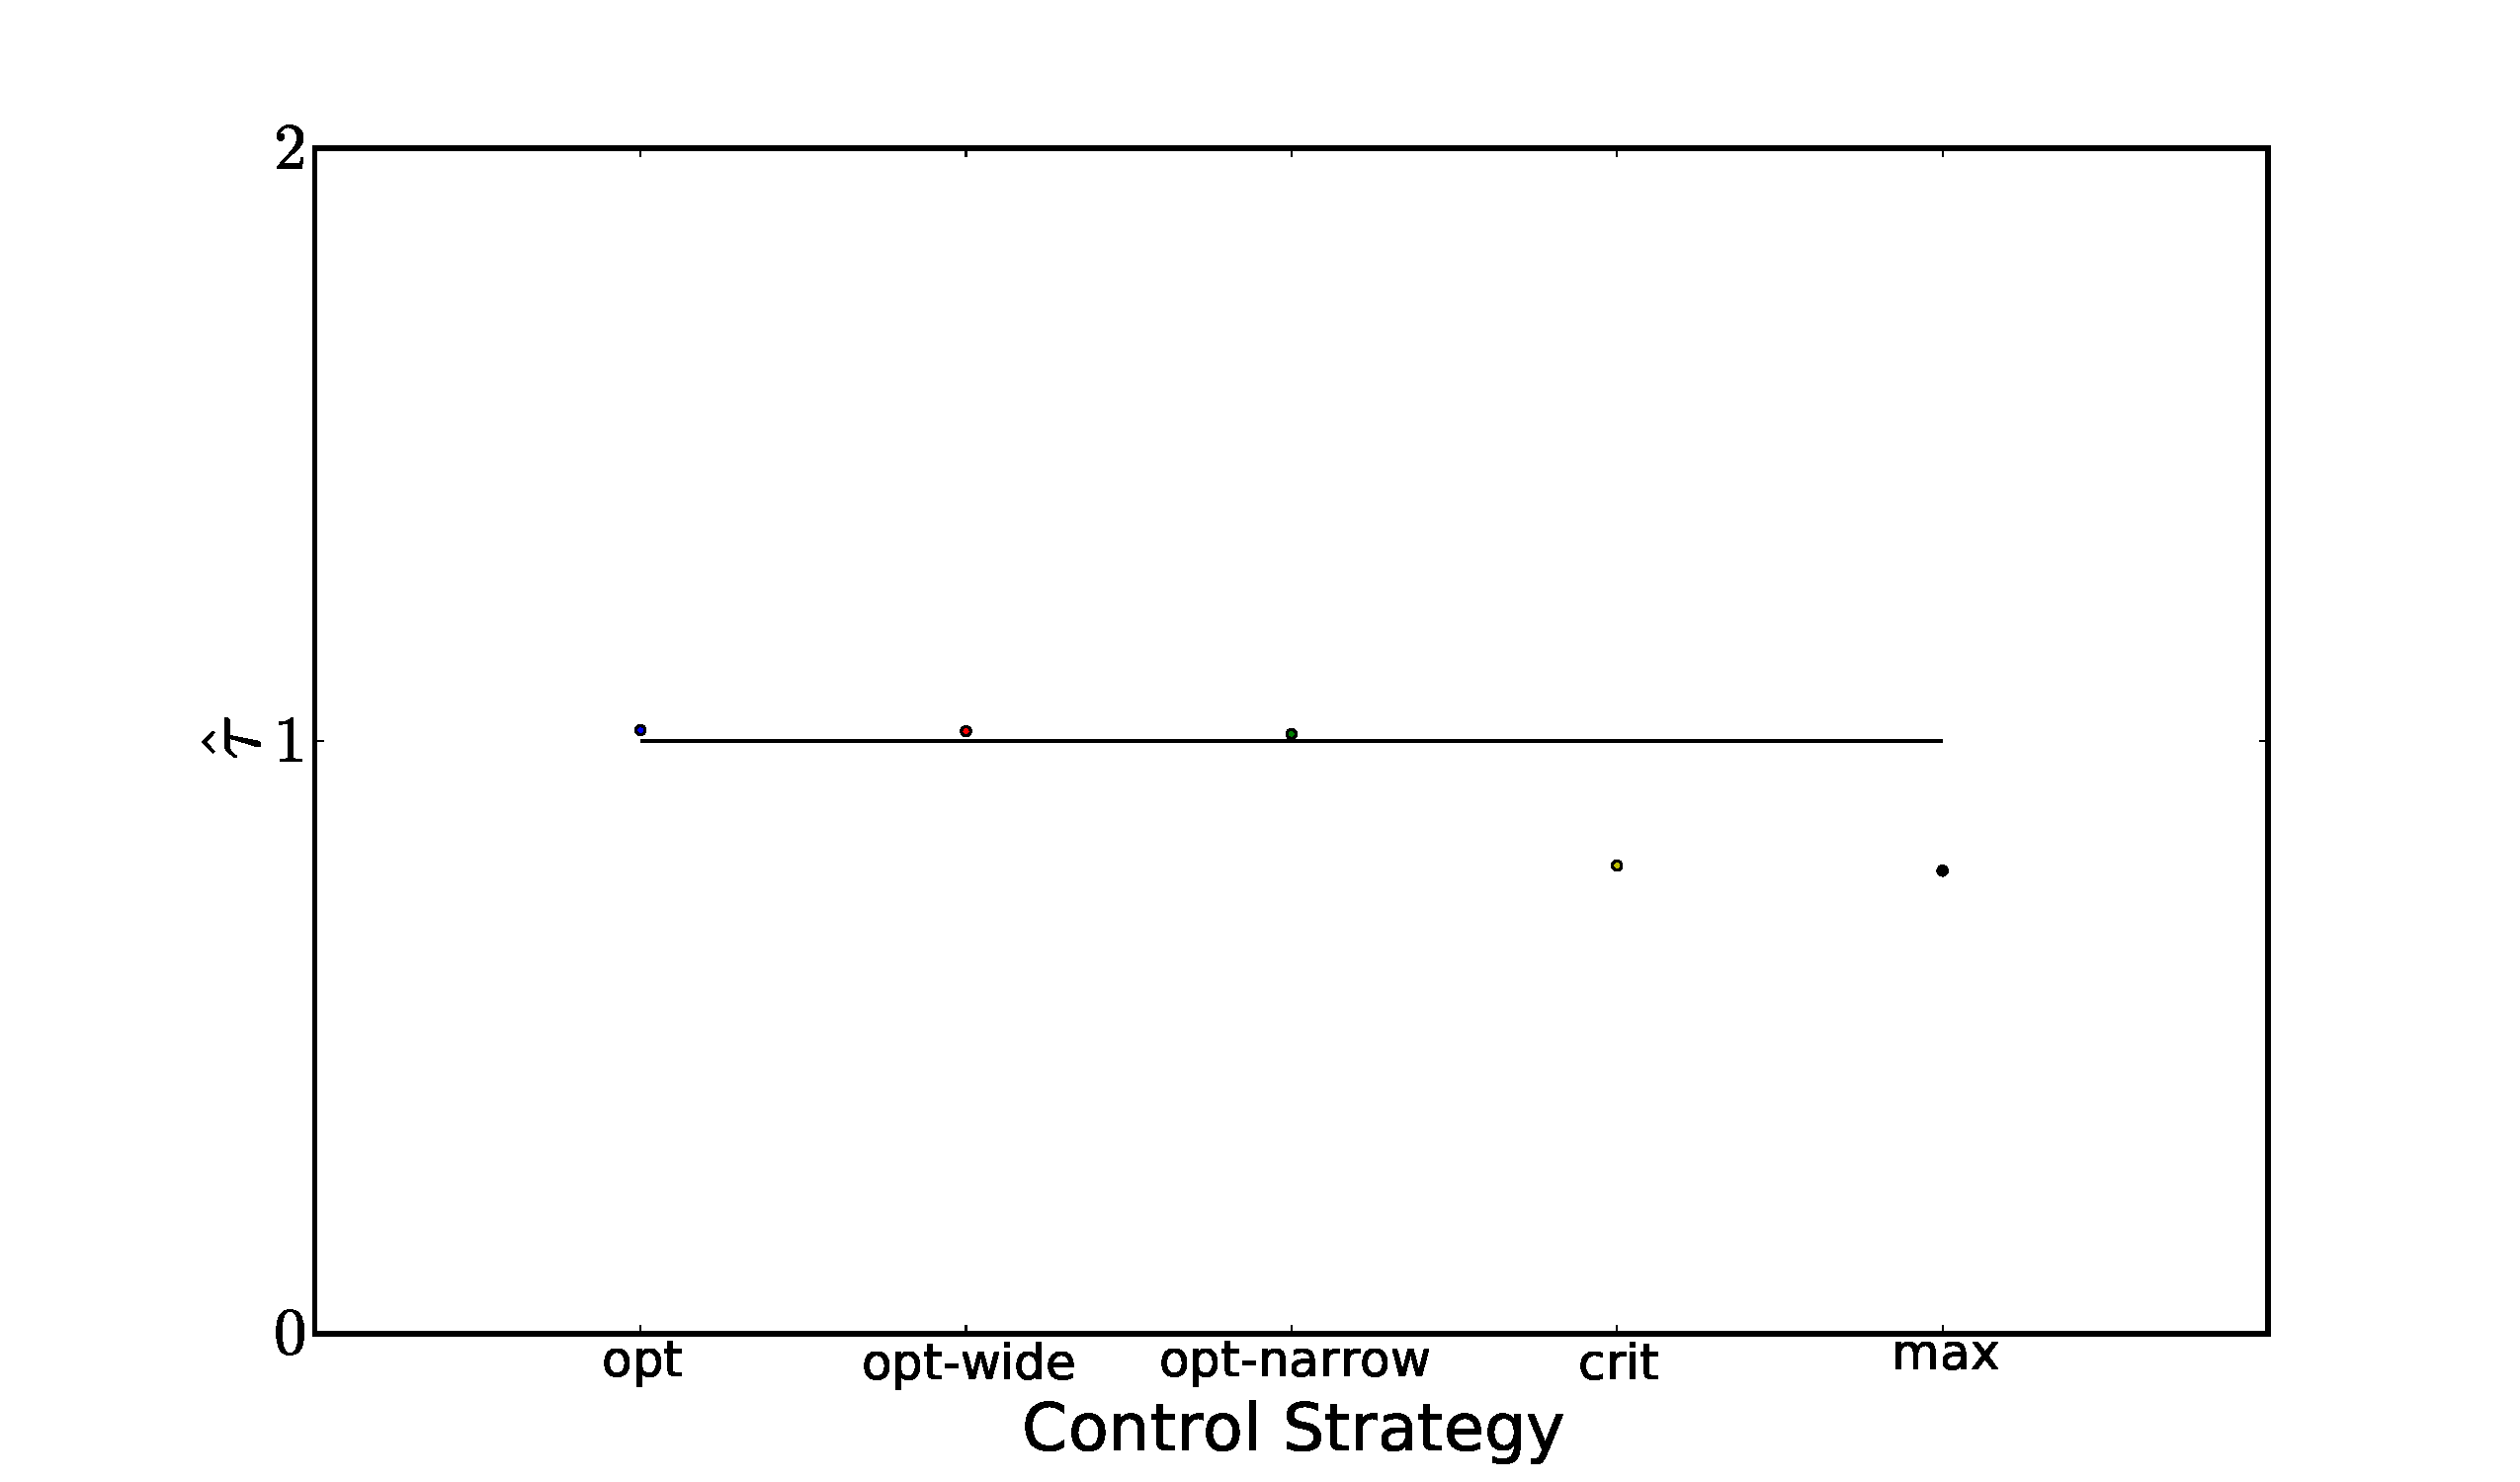
\includegraphics[width=0.48\textwidth]
{Figs/HitTime_MI_TauChar_Adjoint_Estimate/miestimates_scatterplot_Nb1_Ns100000.pdf}
}
\caption[labelInTOC]{Fine Visualization of the MLE estimates for the different
controls also see \cref{tab:beta_estimates_from_hitting_times_different_alphas}}
\label{fig:beta_estimates_from_hitting_times_different_alphas}
\end{center}
\end{figure}

Comments: It certainly looks like there is a marginal advantage to using the 
Optimal Control, $\a_{opt}$ over the simpler, constant controls. In particular
both the bias and variance of the estimates seems to be significantly reduced.
The strange results for $N_s = 100$ require us to look at the actual
distribution of estimates. Results not shown, but the opt-estimates for
$N_s=100$ are bi-modal with a cluster far from the true value. For the higher
$N_s = 1e3,1e4, 1e5$, the opt-estimates are unimodal and tightly centred
around the true value.


\clearpage

\section{Online MI Optimization}
Hеre we outline a tentative approach to {\sl online} optimization of the MI,
which means

\begin{enumerate}
  \item Find $\aopt$ using the gradient ascent, for the prior $\rho$
  \item Apply $\aopt$ and measure several $1,2\ldots,N_{s,1}$ hitting times
  $t_k$
  \item Update the $\rho$ into a posterior conditional on the observed $\{t_k\}$
  \item Recalibrate $\aopt$ using the new $\rho$, i.e. go back to 1. 
\end{enumerate}

 Efficiency considerations aside, we have all the tools to do pts. 1,2,4, it
 is only the prior update that needs to be discussed. 

Of course we start by restating Bayes' formula

$$
\rho(\th| \{t_k\} ) = 
\frac{  \rho(\th) \cdot \prod_k g(t_k|\th ; \a) }
	 { \int_\Th  \rho(\th) \cdot \prod_k g(t_k|\th ; \a)  \intd{\th}}
$$

In practice, exact calculation of $\rho(\th|\t_k)$ would not be possible in our
context, so an approximation approach needs to be made.

The standard approach is to describe the belief distribution by an ensemble of
points (particles). We now describe the basic aspect of how the particle
ensemble is constructed, how it is updated and how it is resampled. We use the
reference \cite{Granade2012}, in particular sec 4 therein.

\subsection{Quick INtro to Particle Filtering}
We have a prior
$ \rho(\th)$ and we want to describe it by an ensemble of points $\th_i$.
as 
$$ \rho(\th) \sim \sum_i w_i \delta(\th-\th_i)$$
This is what we have been doing up to now for the MI optimization routines.

Again recall that a bayesian update, given the $k$th hitting time is
$$ \rho(\th|t_k) \propto g(t_k|\th)\rho(\th)$$

thus the weights are iteratively updated as 

$$w_i \ra w_i g(t_k|\th_i)$$

Given the particle ensemble, $\{\th_i, w_i\}$, we can  then approximate the
mean/variance of $\Th$ as
$$ \Exp[\Th] \approx \sum_i w_i \th_i$$
and 
$$ \Var[\Th] \approx \sum_i w_i \th_i \th_i - (\Exp[\Th])^2$$
In fact, in general 
$$\Exp[f(\Th)]\approx\sum_i w_i f(\th_i)$$ approximates the expectation of any
function, $f$, of the random variable $\Th$.

Here's the crux of the update/resample algorithm. Given a new observation, i.e.
the latest hitting time $t_k$, the weights are updated according to
$$ w_{i,k} = w_{i,k-1}\cdot g(t_k| \th_i, \a_k),$$where $g(|\th_i, \a_k)$ is
the probability density given the parameter value $\th_i$ and the chosen
stimulation that was applied during the $k$th sample, $\a_k(\cdot)$.
The weights are then re-normalized so that at all time $$\sum_i w_i = 1$$ 

The literature suggests that this procedure will tend to concentrate all the
'mass' on one location and most of the weights will decrease to 0. This
concentration is 'bad' since eventually, all the weights go to zero and so
effectively the distribution has converged  artificially to a point, which might
be the most likely point from the initial ensemble, but still be far from the
'true' value of the parameter. This adverse effect can be ameliorated by
resampling the {\sl locations} of the particle ensemble, $\th_i$. This
resampling can be done in many ways, but a standard way is described in
algorithm. \ref{alg:particle_resampling} (which is copied from Algo4 in Granade
et. al. \cite{Granade2012}, who in turn closely follow \cite{Liu2001}, but
are very nice and pedagogical).
\begin{algorithm}
\begin{algorithmic}
\State Given  $\{w_i, \th_i\}_1^N_p$ the current particle ensemble (weight,
locations)  
\State $\m $ \gets $\Exp[\Th]$ 
\State $a = 0.98$ see \cite{Granade2012,Liu2001}
\State $h = \sqrt{1-a^2}$ i.e. $h \approx 0.1990$
\State $\Xi$\gets $h^2\cdot \Var[\Th]$
\For {$i= 1\dots N_p$}
	\\ {\itshape $\#$ Re-sample each particle individually}
	\State draw $j$ with probability $w_j$ 
	\\ {\itshape $\#$ the bigger $w_i$ the more likely to choose
	$\th_i$}
	\State $m_i$ \gets  $a \th_j + (1-a) \m$
	\State Resample $\th_i'$ from $N(\m_i, \Xi)$
	\State $w_i$ \gets $1/N_p$ 
    \EndFor{\itshape $\quad \#   1 \ldots N_p$ particle resampling}
\State \Return $w_i, \th_i'$ the resampled particle ensemble 
\end{algorithmic}
\caption{Particle Resampling Algorithm}
\label{alg:particle_resampling}
\end{algorithm}

While, of course, updating happens after every iteration, re-sampling happens
only when  
$$ \frac{1}{\sum_i^{N_p} w_i^2} < \frac {N_p}{2} \implies \textrm{ resample!}$$

In \cref{fig:poissonian_rate_filtering} we give an example for the filtering
procedure to estimate the rate of a Poissonian process, $1/\t$, for which  the
likelihood is just $\tfrac 1\t exp(- \tfrac t\t)$. From
\cref{fig:poissonian_rate_filtering} we can conclude that the basic mechanics of
the filtering update/resample procedure is working. (We've tried it with other
values of $\tau$ and it works for those as well.)

%\usepackage{graphics} is needed for \includegraphics
\begin{figure}[htp]
\begin{center}
  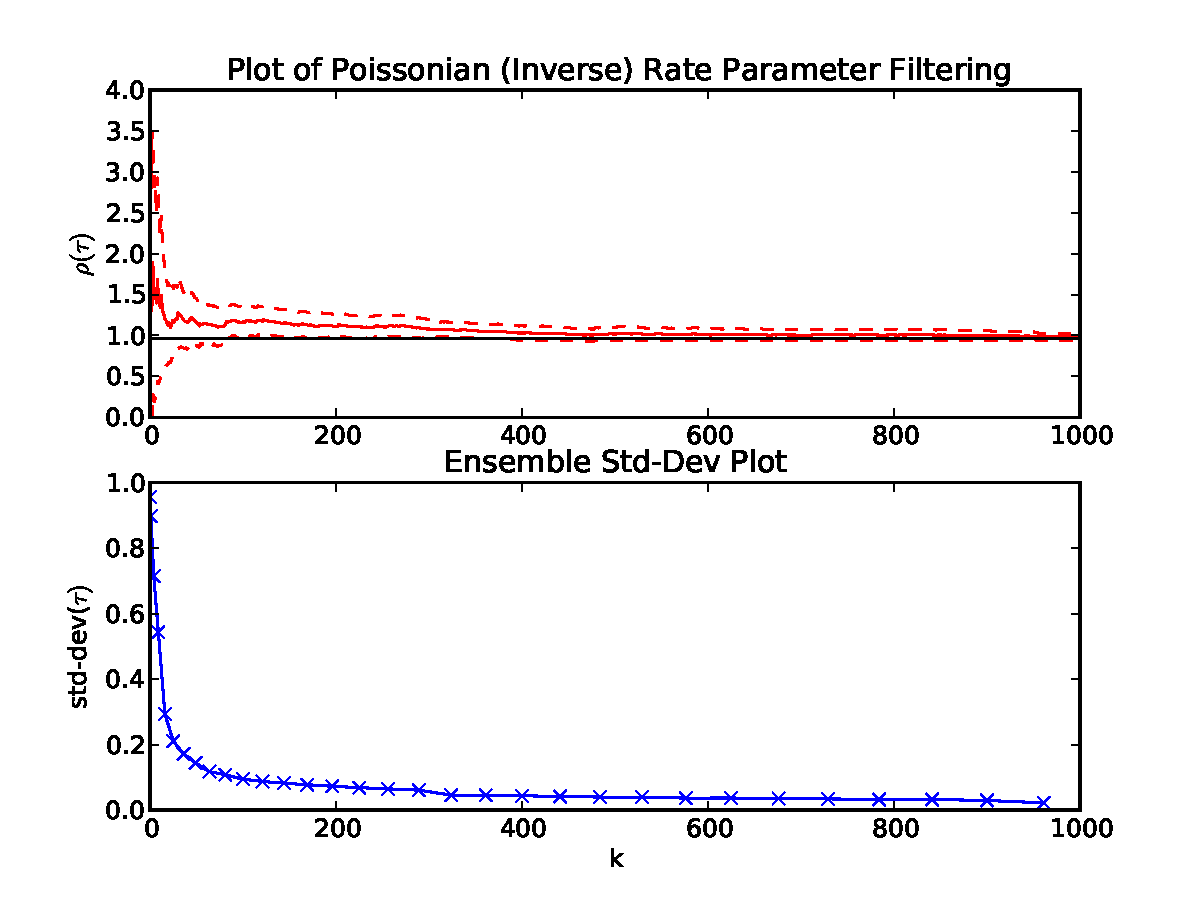
\includegraphics[width=\textwidth]{Figs/TauParticleEnsemble/poisson_rate_filtering.pdf}
  \caption{Filtering Example for a test-case. We are trying to estimate the
  inverse of the Poissonian rate, $1/\tau$, given inter-event intervals $t_k$.
  The true value is $\tau  = 1$. The Maximum Likelihood estimate for $\tau$ in
  this problem  is just the mean of the observed times $\bar{t_k}$, which
  happens to be 0.9583 in this example, while after the last observation, the
  ensemble mean $\pm$ std-dev is $0.9811\pm 0.0199$}
  \label{fig:poissonian_rate_filtering}
\end{center}
\end{figure}

% \clearpage

\subsection{Example of Particle-Filtering + Online Estimation for hitting time
parameter estimation}

\subsubsection{Single HItting Time Illustration}
Let's try it. First, in \cref{fig:example_online_miopt_single_iteration}, we
illustrate one iteration of the update, that is one hitting time given a
stimulation from either the MI Optimal Controller or a random controller, which
just gives a random constant stimulation per each hitting time.

Let's discuss what happens in \cref{fig:example_online_miopt_single_iteration}.
Recall that lower values of $\tc$ imply higher restoring force and therefore
longer hitting times (waiting times). Since in this sample, the observed hitting
times were fairly long, especially for the MI-optimal stimulation, weights for
smaller $\t$s grow larger, while weights for bigger $\t$s become smaller.
However it is immediately clear that the MI-optimal stimulation is more
discerning as it has almost entirely discarded (correctly) the
possibility that $\tau>2$, while the other two stimulations have resulted in
only mild perturbation in the belief distribution. 

WARNING: The new results are much better primarily through a judicious choice of
the initial condition of the MI-optimal optimization (the initial guess for the
optimal control.)

\begin{figure}[h]
\begin{center}
\subfloat[Example Hitting Times]
{
\label{fig:example_hitting_times_for_online_miopt}
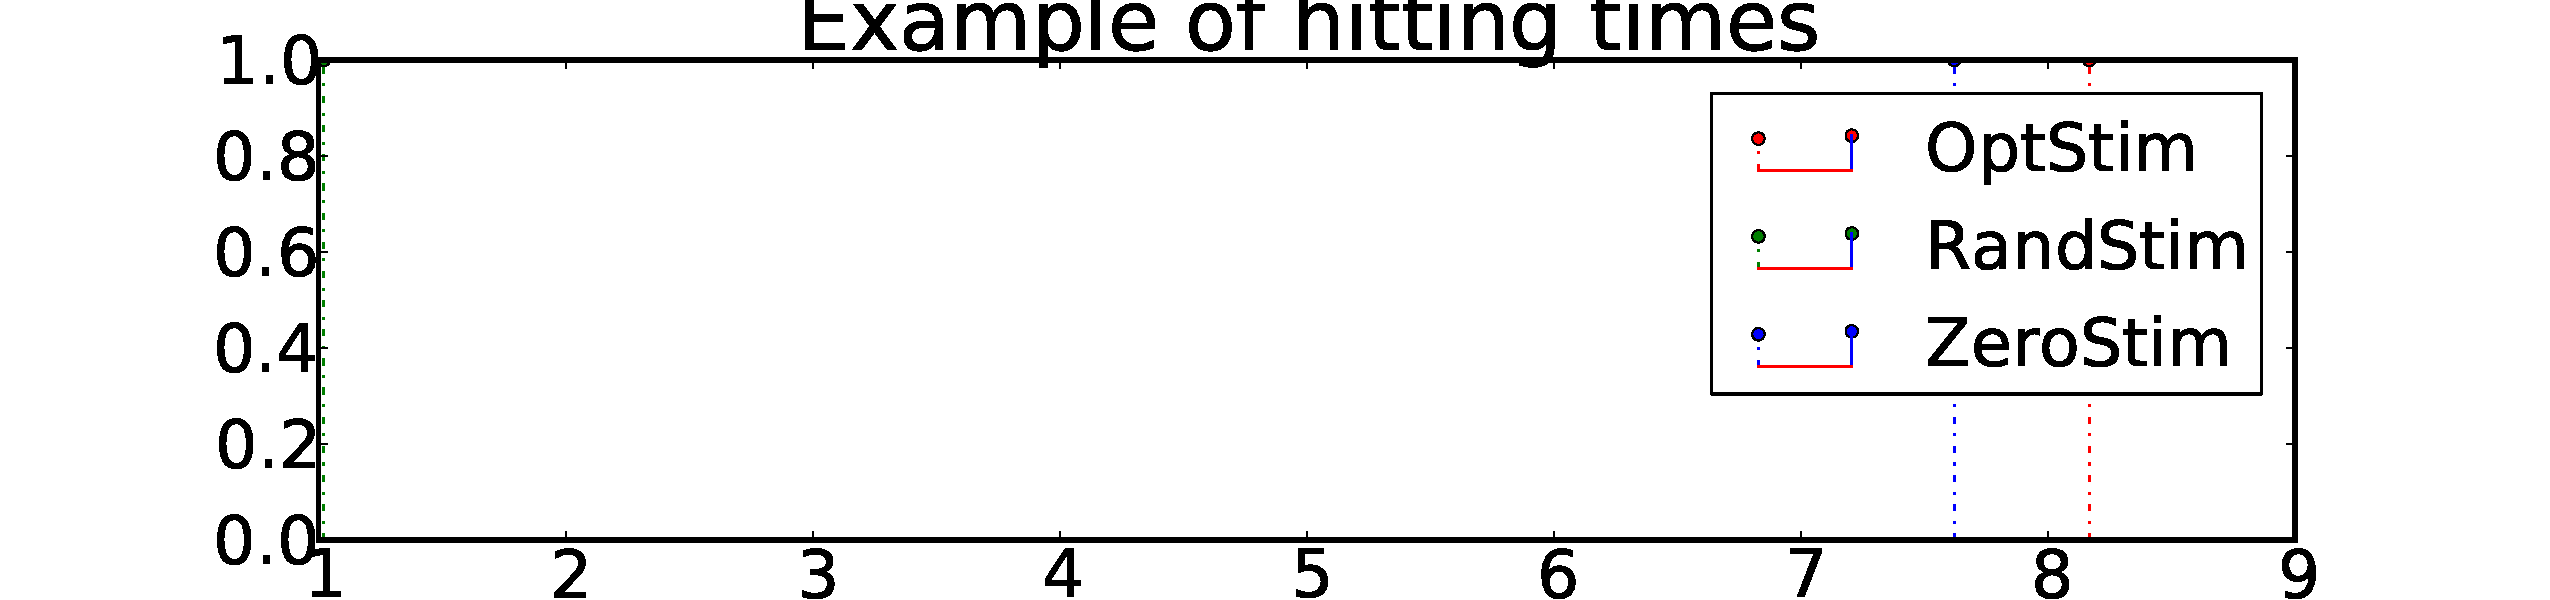
\includegraphics[width=0.48\textwidth]
{Figs/HTOnlineEstimator/single_trial_example_hittimes.pdf}
} 
\subfloat[Resulting Particle Ensemble Updates]
{
\label{fig:example_particle_ensemble_updates_for_online_miopt}
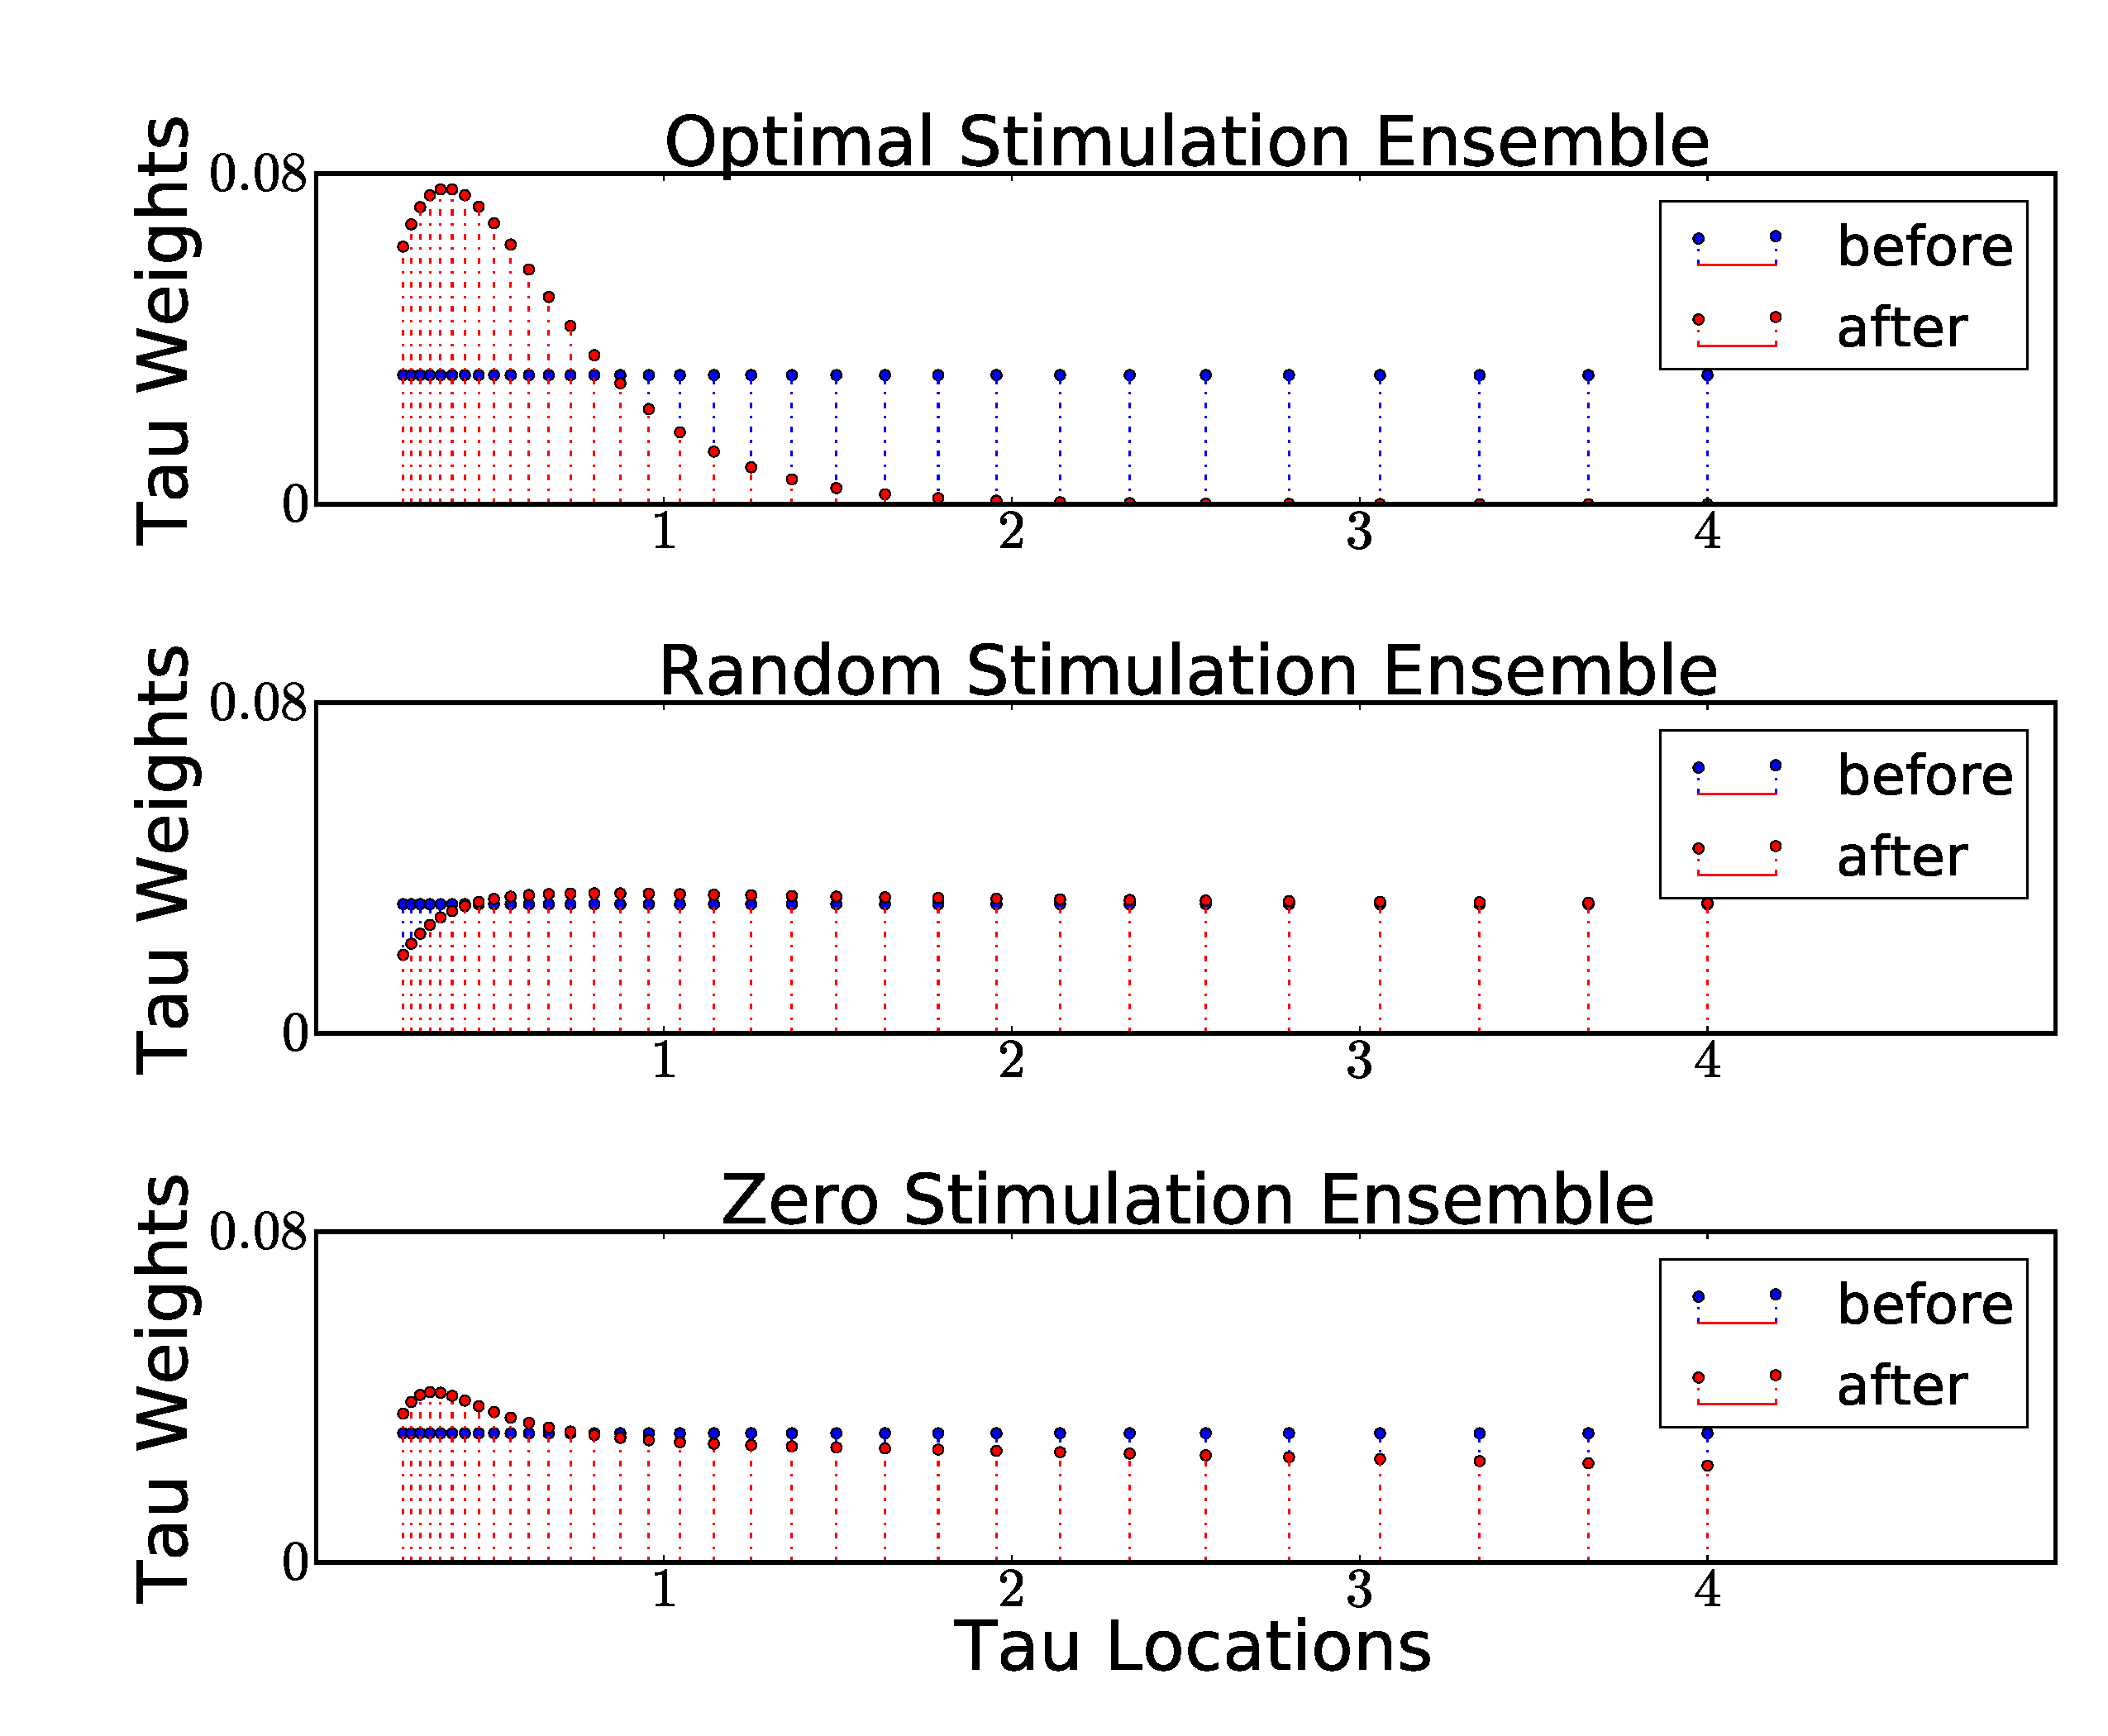
\includegraphics[width=0.48\textwidth]
{Figs/HTOnlineEstimator/single_trial_example_weights.pdf}
}
\caption[labelInTOC]{Examples of a single iteration of the Online
Stimulation-Estimation scheme.  }
\label{fig:example_online_miopt_single_iteration}
\end{center}
\end{figure}

\subsubsection{Full Multiple Hitting-Times Experiment(s)}
Now let's go through an entire estimation experiment. That is let's stimulate a
sequence of hitting times and online update our parameter belief distribution,
after every observation and then online-update our MI-optimal stimulation as the
belief evolves.

The main result is shown in \cref{fig:example_miopt_vs_rand_ensemble_evolution},
where we visualize the mean and confidence intervals for the belief
distributions for the three protocols (MI-Optimal vs. Random Constant vs Zero),
using $N_\t = 32$ particles and $N_k=251$ hitting times. In
\cref{fig:example_miopt_controls_evolution}, we show the different stimulations
that were chosen by the Mutual-Info Maximization Algorithm.
 
\begin{figure}[htp]
\begin{center}
  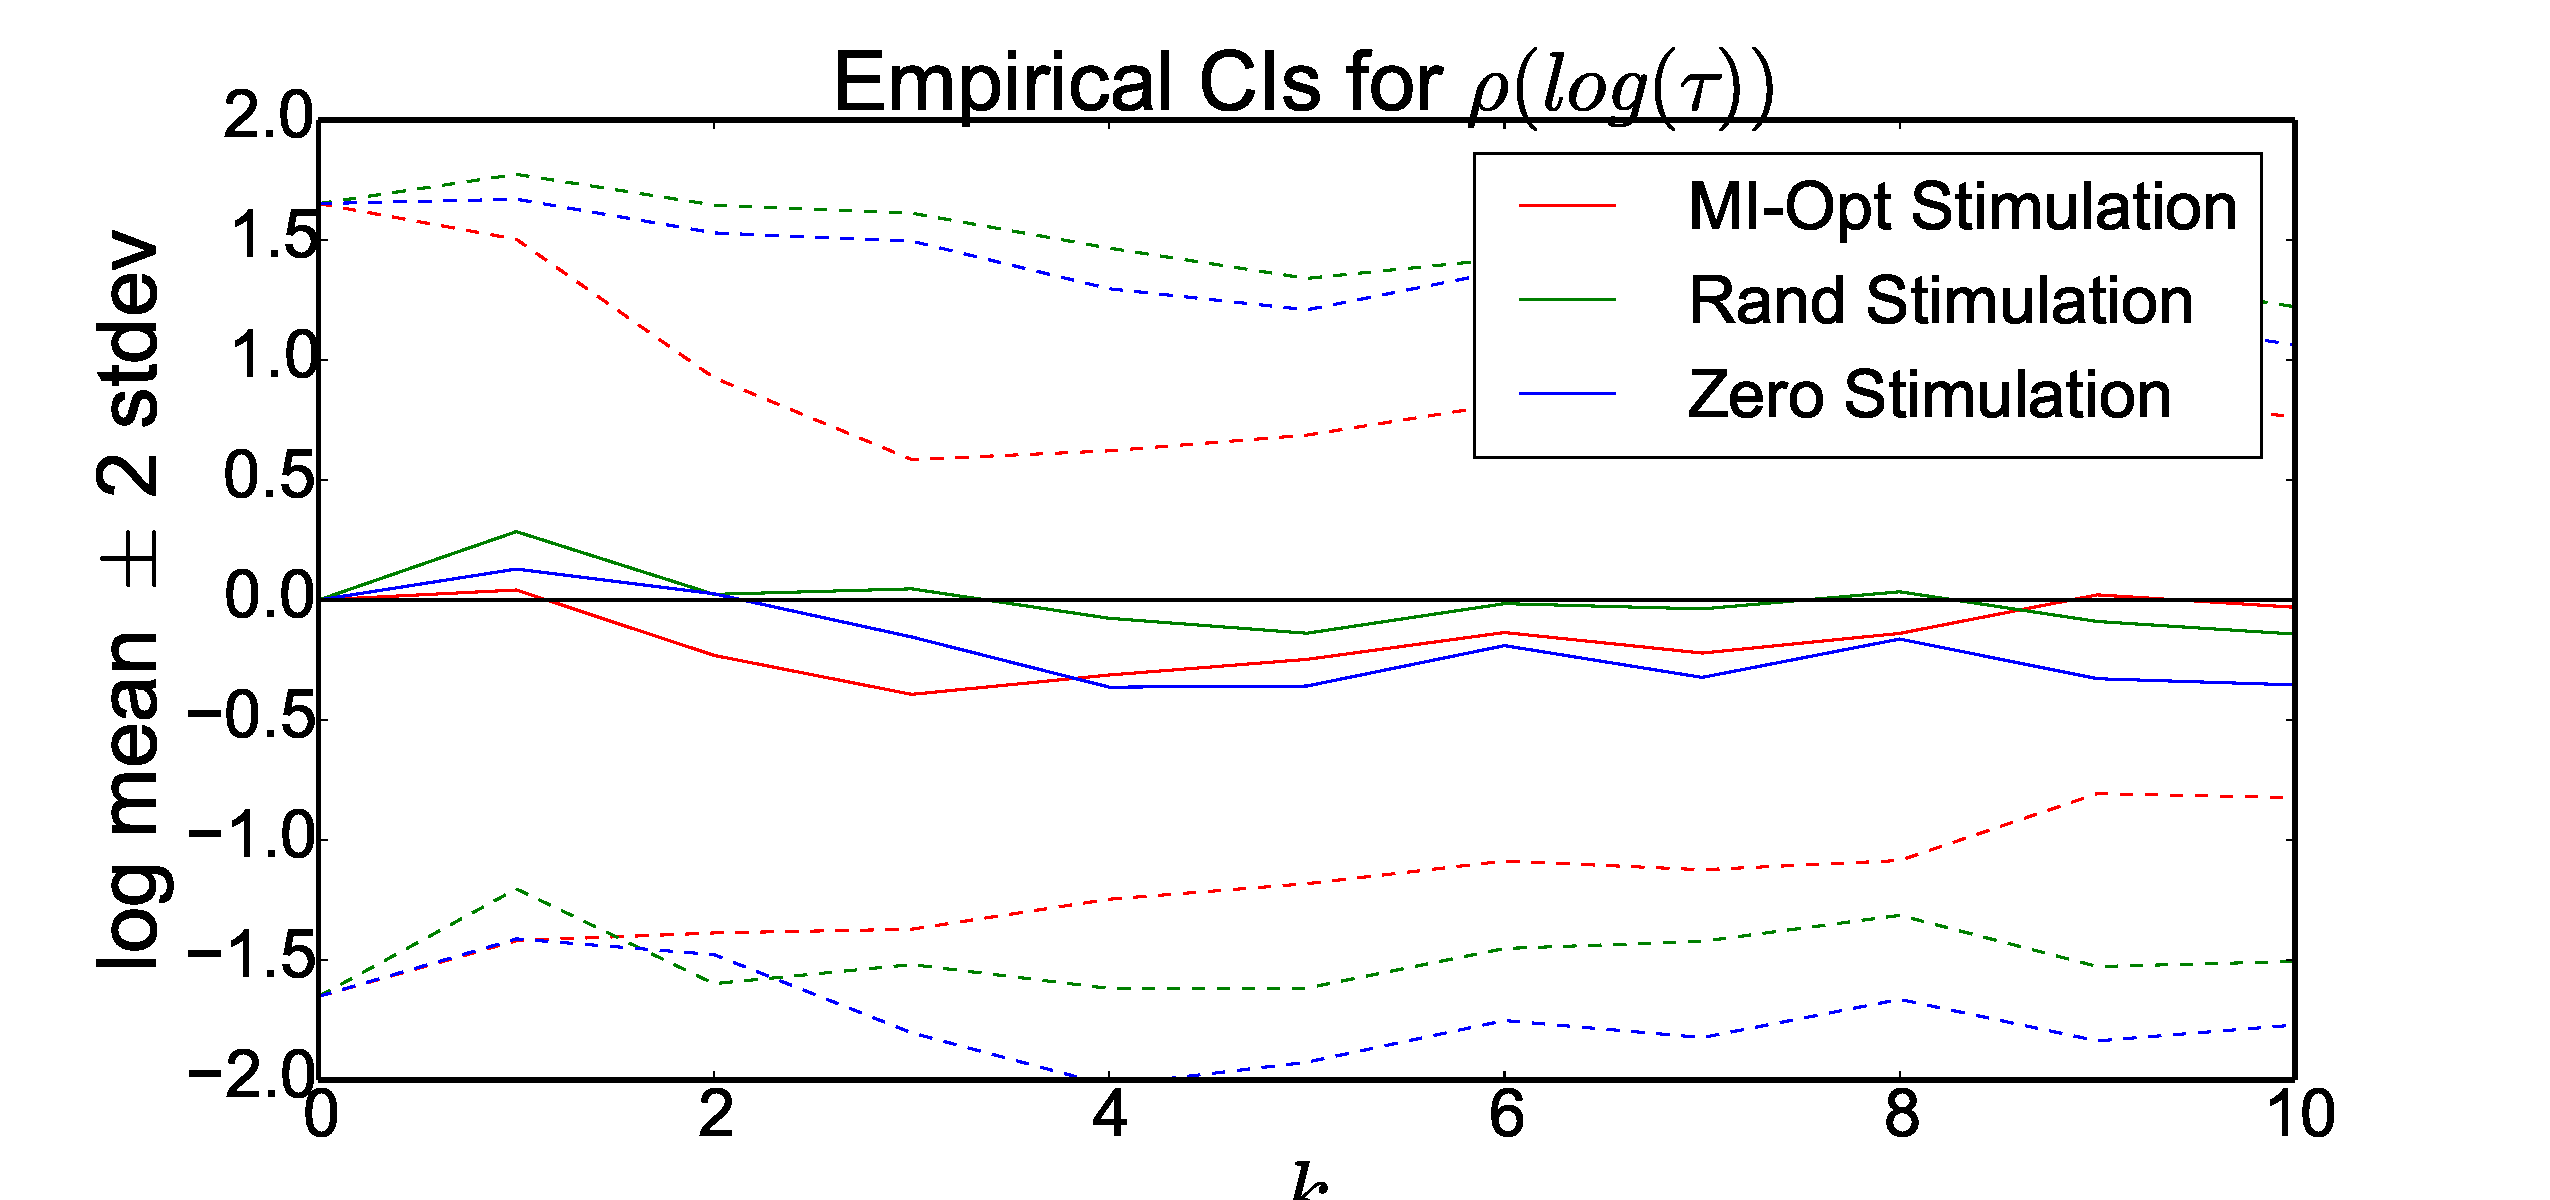
\includegraphics[width=\textwidth]{Figs/HTOnlineEstimator/single_experiment_example_ensemble_distn_evolution.pdf}
  \caption[labelInTOC]{Evolution of the belief distributions given Optimal
  (red) or Random (green) stimulation. We used $N=32$ particles to represent
  the ensemble for both stimulation protocols. There are 250 hitting times used}
  \label{fig:example_miopt_vs_rand_ensemble_evolution}
\end{center}
\end{figure}
\begin{figure}[htp]
\begin{center}
  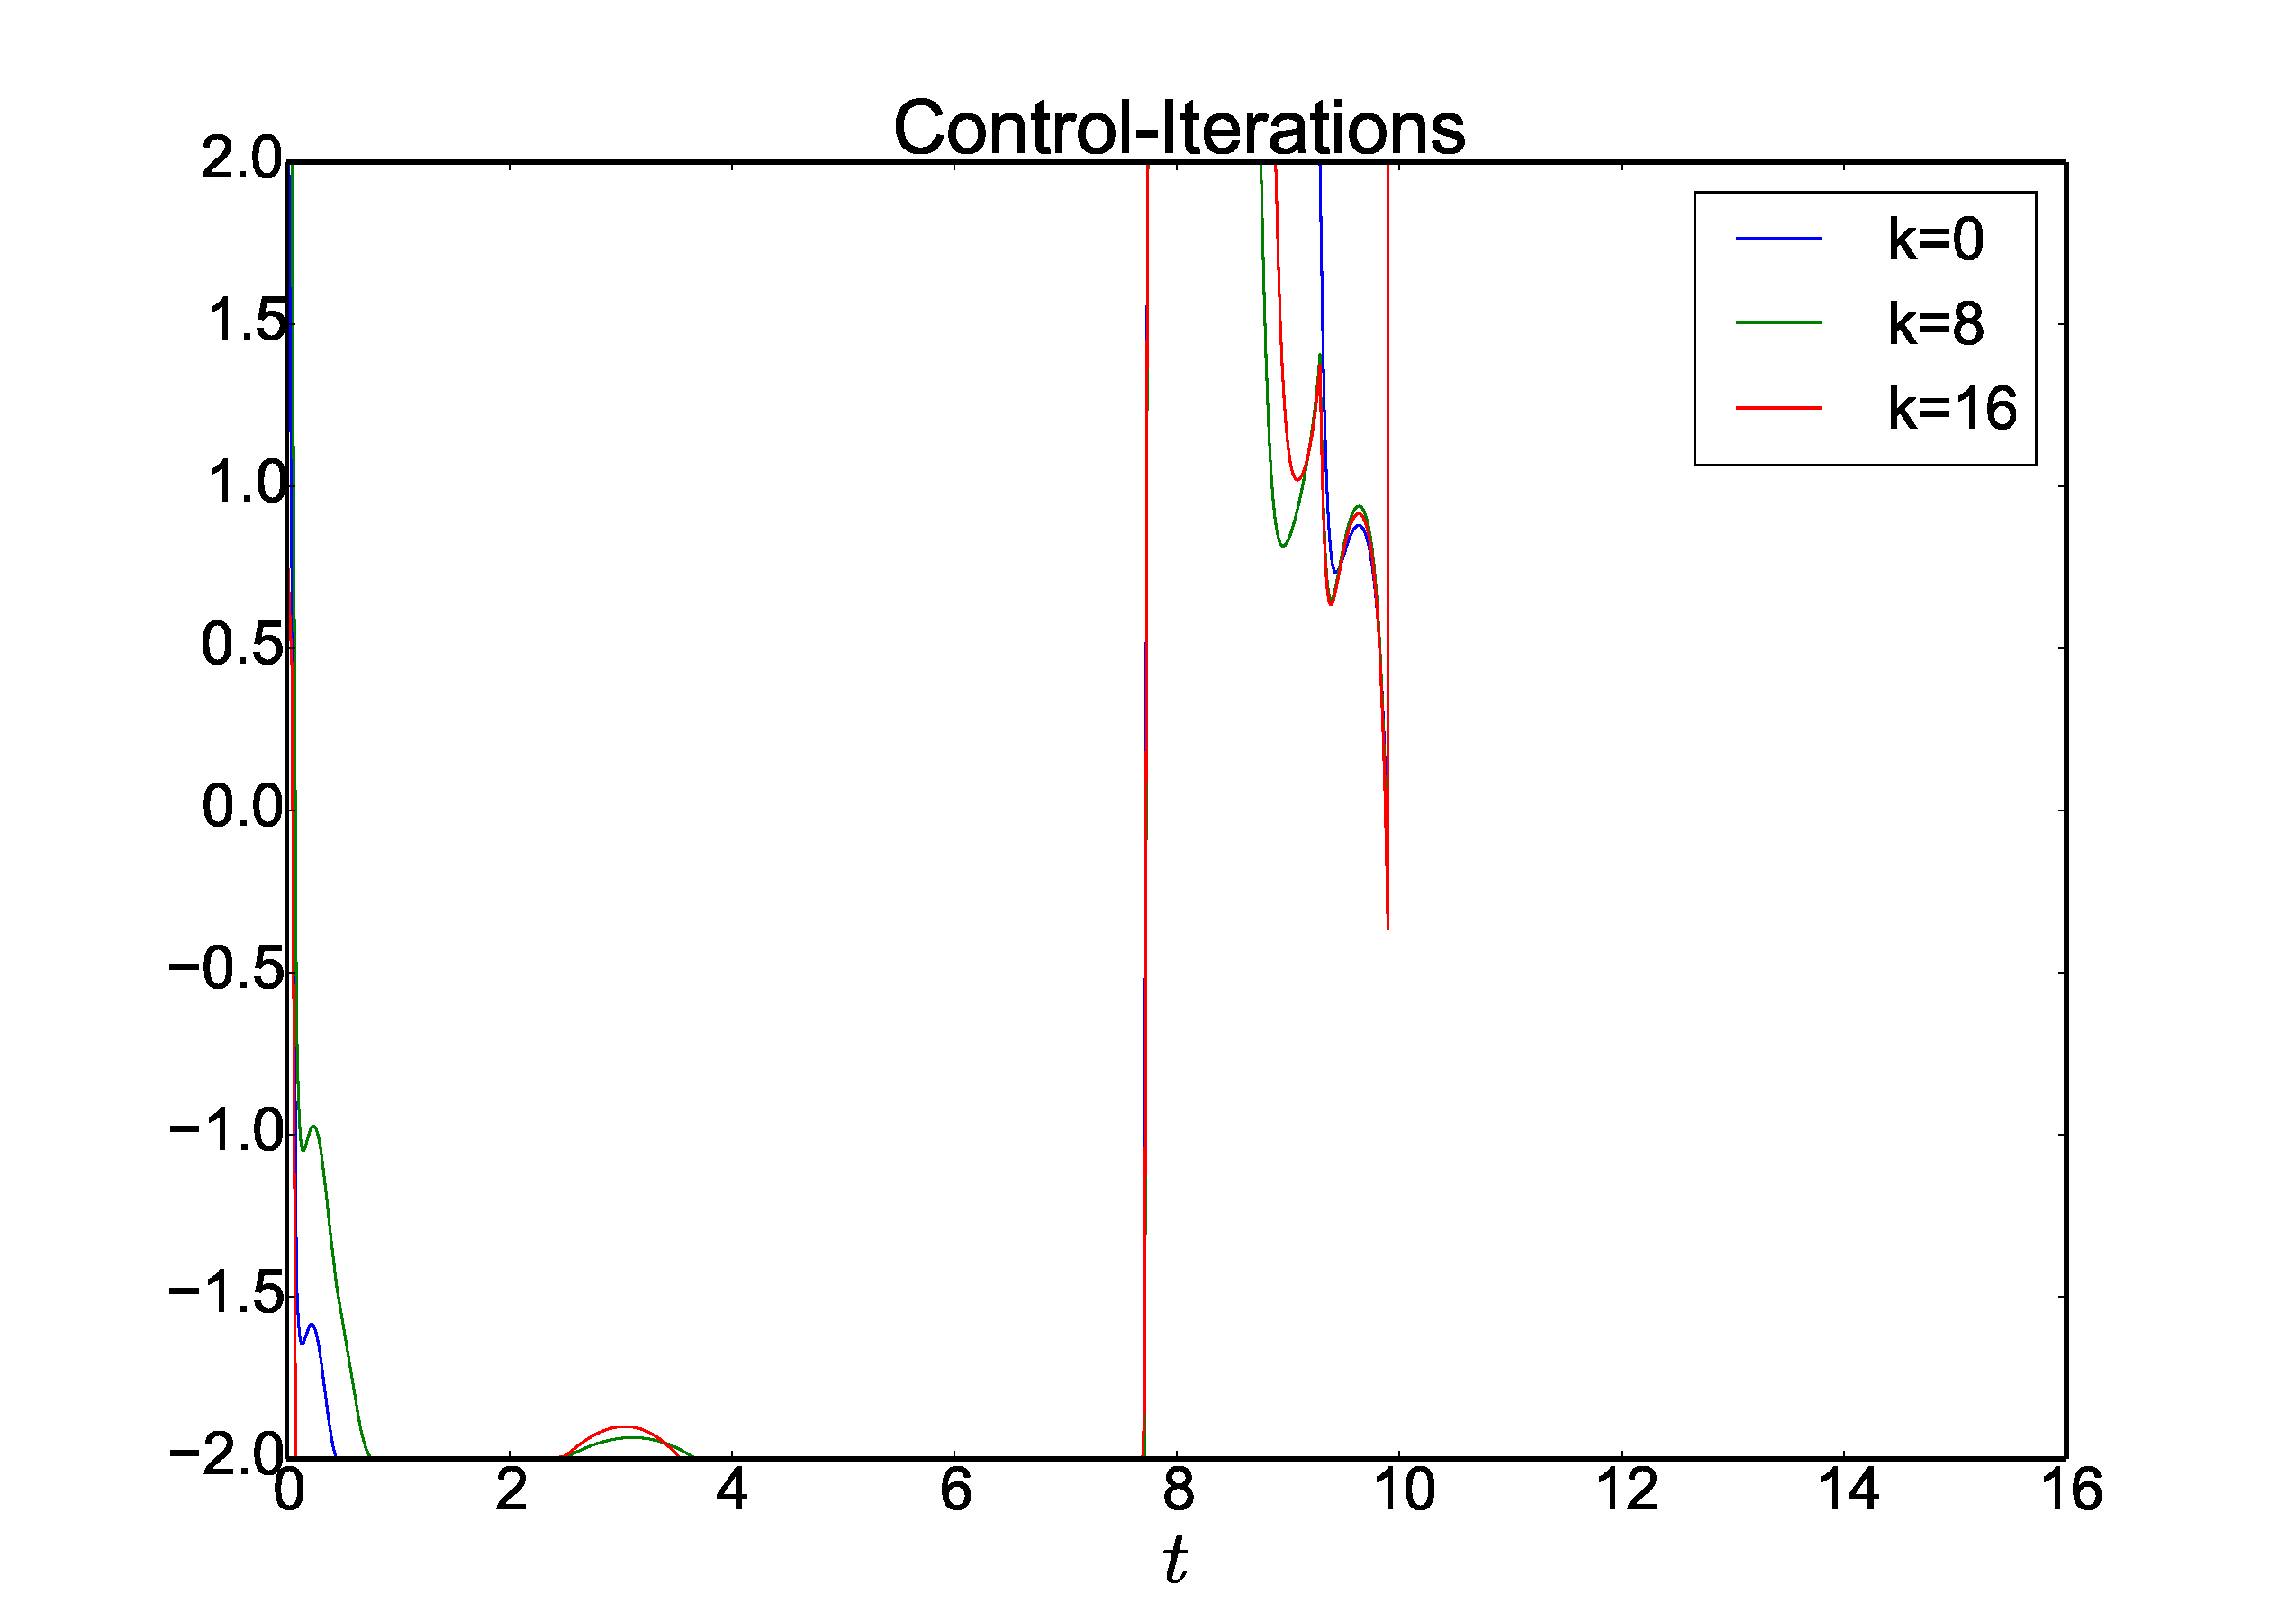
\includegraphics[width=\textwidth]{Figs/HTOnlineEstimator/single_experiment_example_controls_evolution.pdf}
  \caption[labelInTOC]{Different MI-OPtimal Stimulations computed 
  as the Experiment evolves and the parameter belief distribution changes}
  \label{fig:example_miopt_controls_evolution}
\end{center}
\end{figure}
 

\clearpage

We now simulate $10$ independent experiments of approx. 500 hitting times each
and visualize them in \cref{fig:online_optimization_more_examples}. Here, we see
that the MI-optimal stimulation is indeed producing more accurate
estimates, faster (earlier in the experiment). This is true in 7 out of the 10
experiments, in 2 it is hard to determine whether there is a 'better' protocol
and only once is the MI-based stimulation resulting in worse estimates than one
of the alternatives ((f) in \cref{fig:online_optimization_more_examples}). 
 
\begin{figure}[h]
\begin{center}
\subfloat[]
{
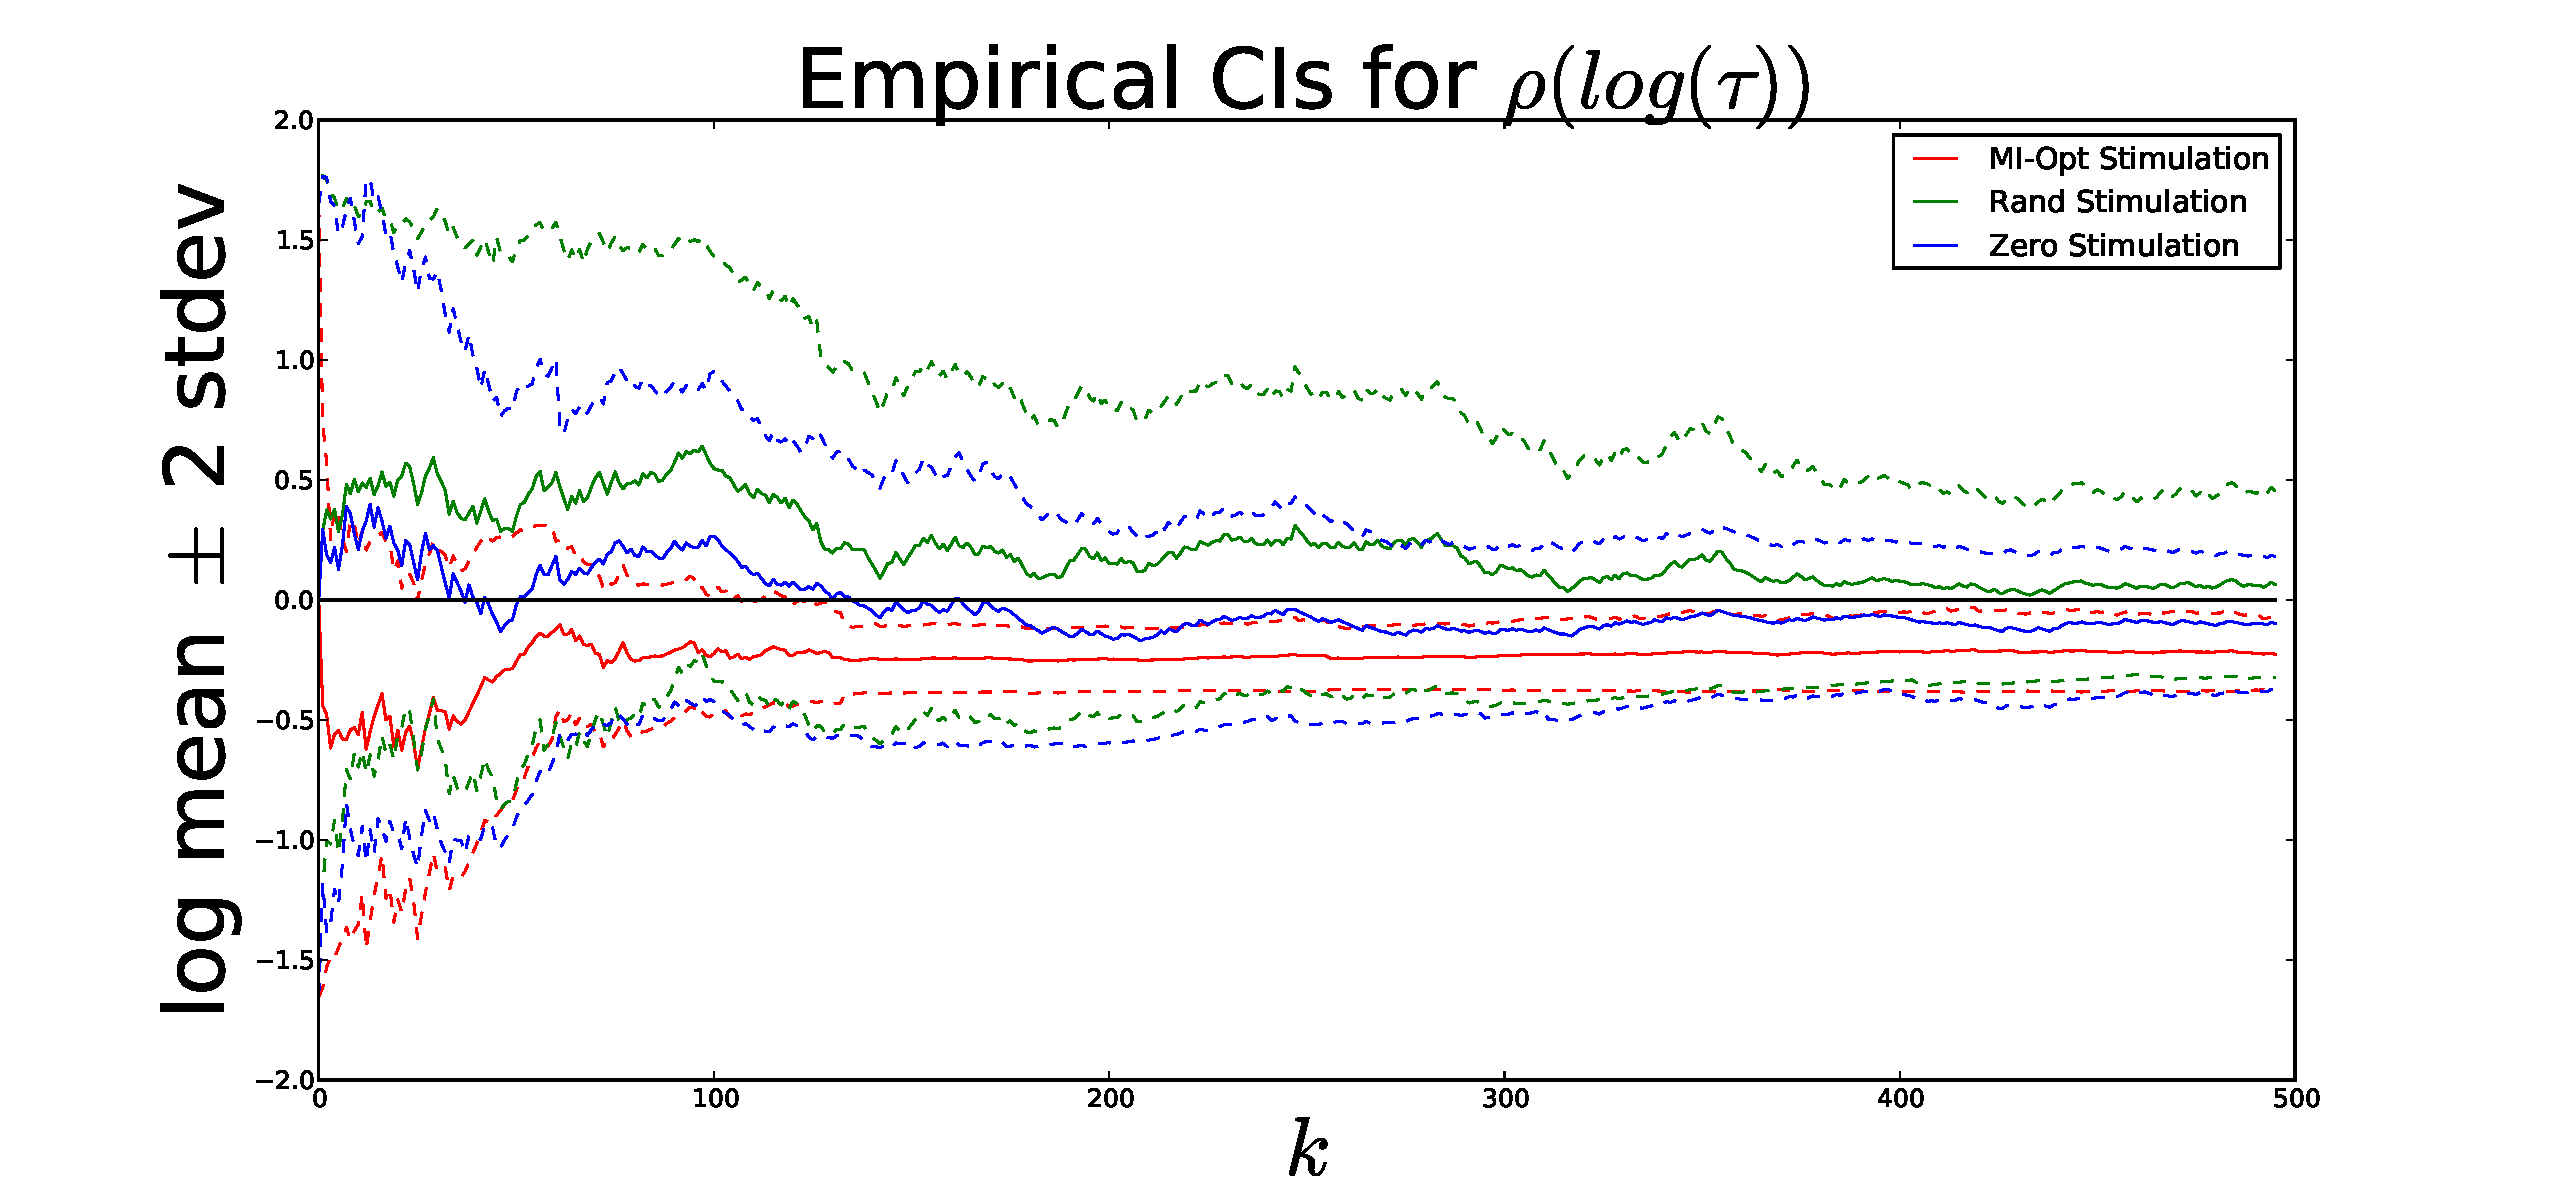
\includegraphics[width=0.48\textwidth]
{Figs/HTOnlineEstimator/single_experiment_exampleNts=32_Ntrls=495_ensemble_distn_evolution.pdf}
}
\subfloat[]
{
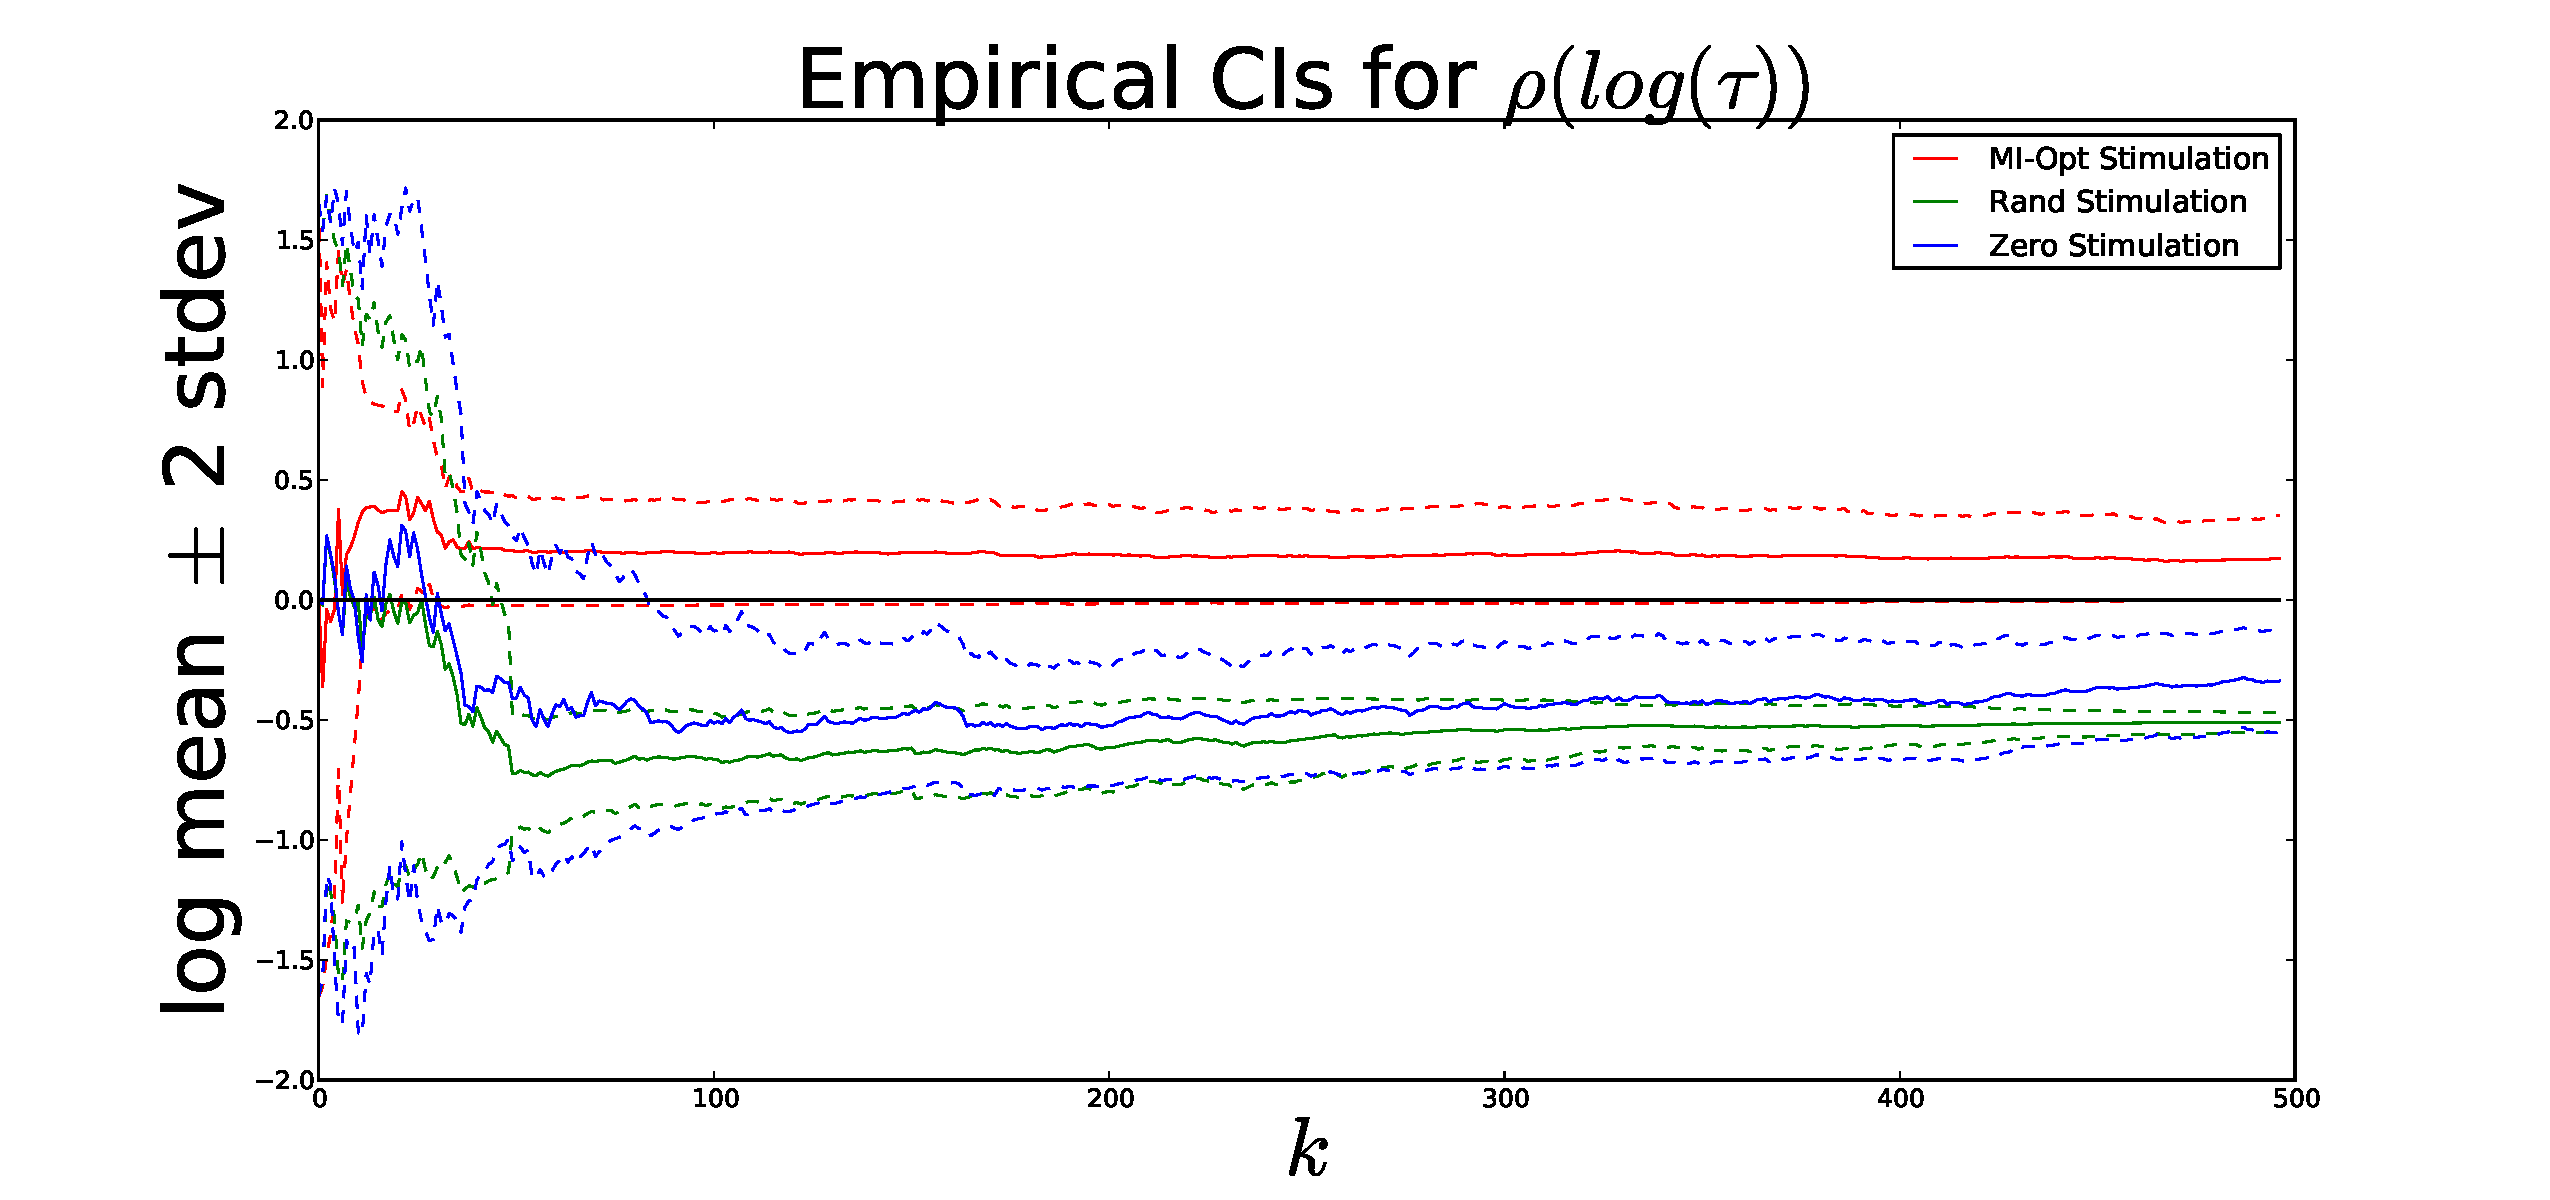
\includegraphics[width=0.48\textwidth]
{Figs/HTOnlineEstimator/single_experiment_exampleNts=32_Ntrls=496_ensemble_distn_evolution.pdf}
}\\
\subfloat[]
{
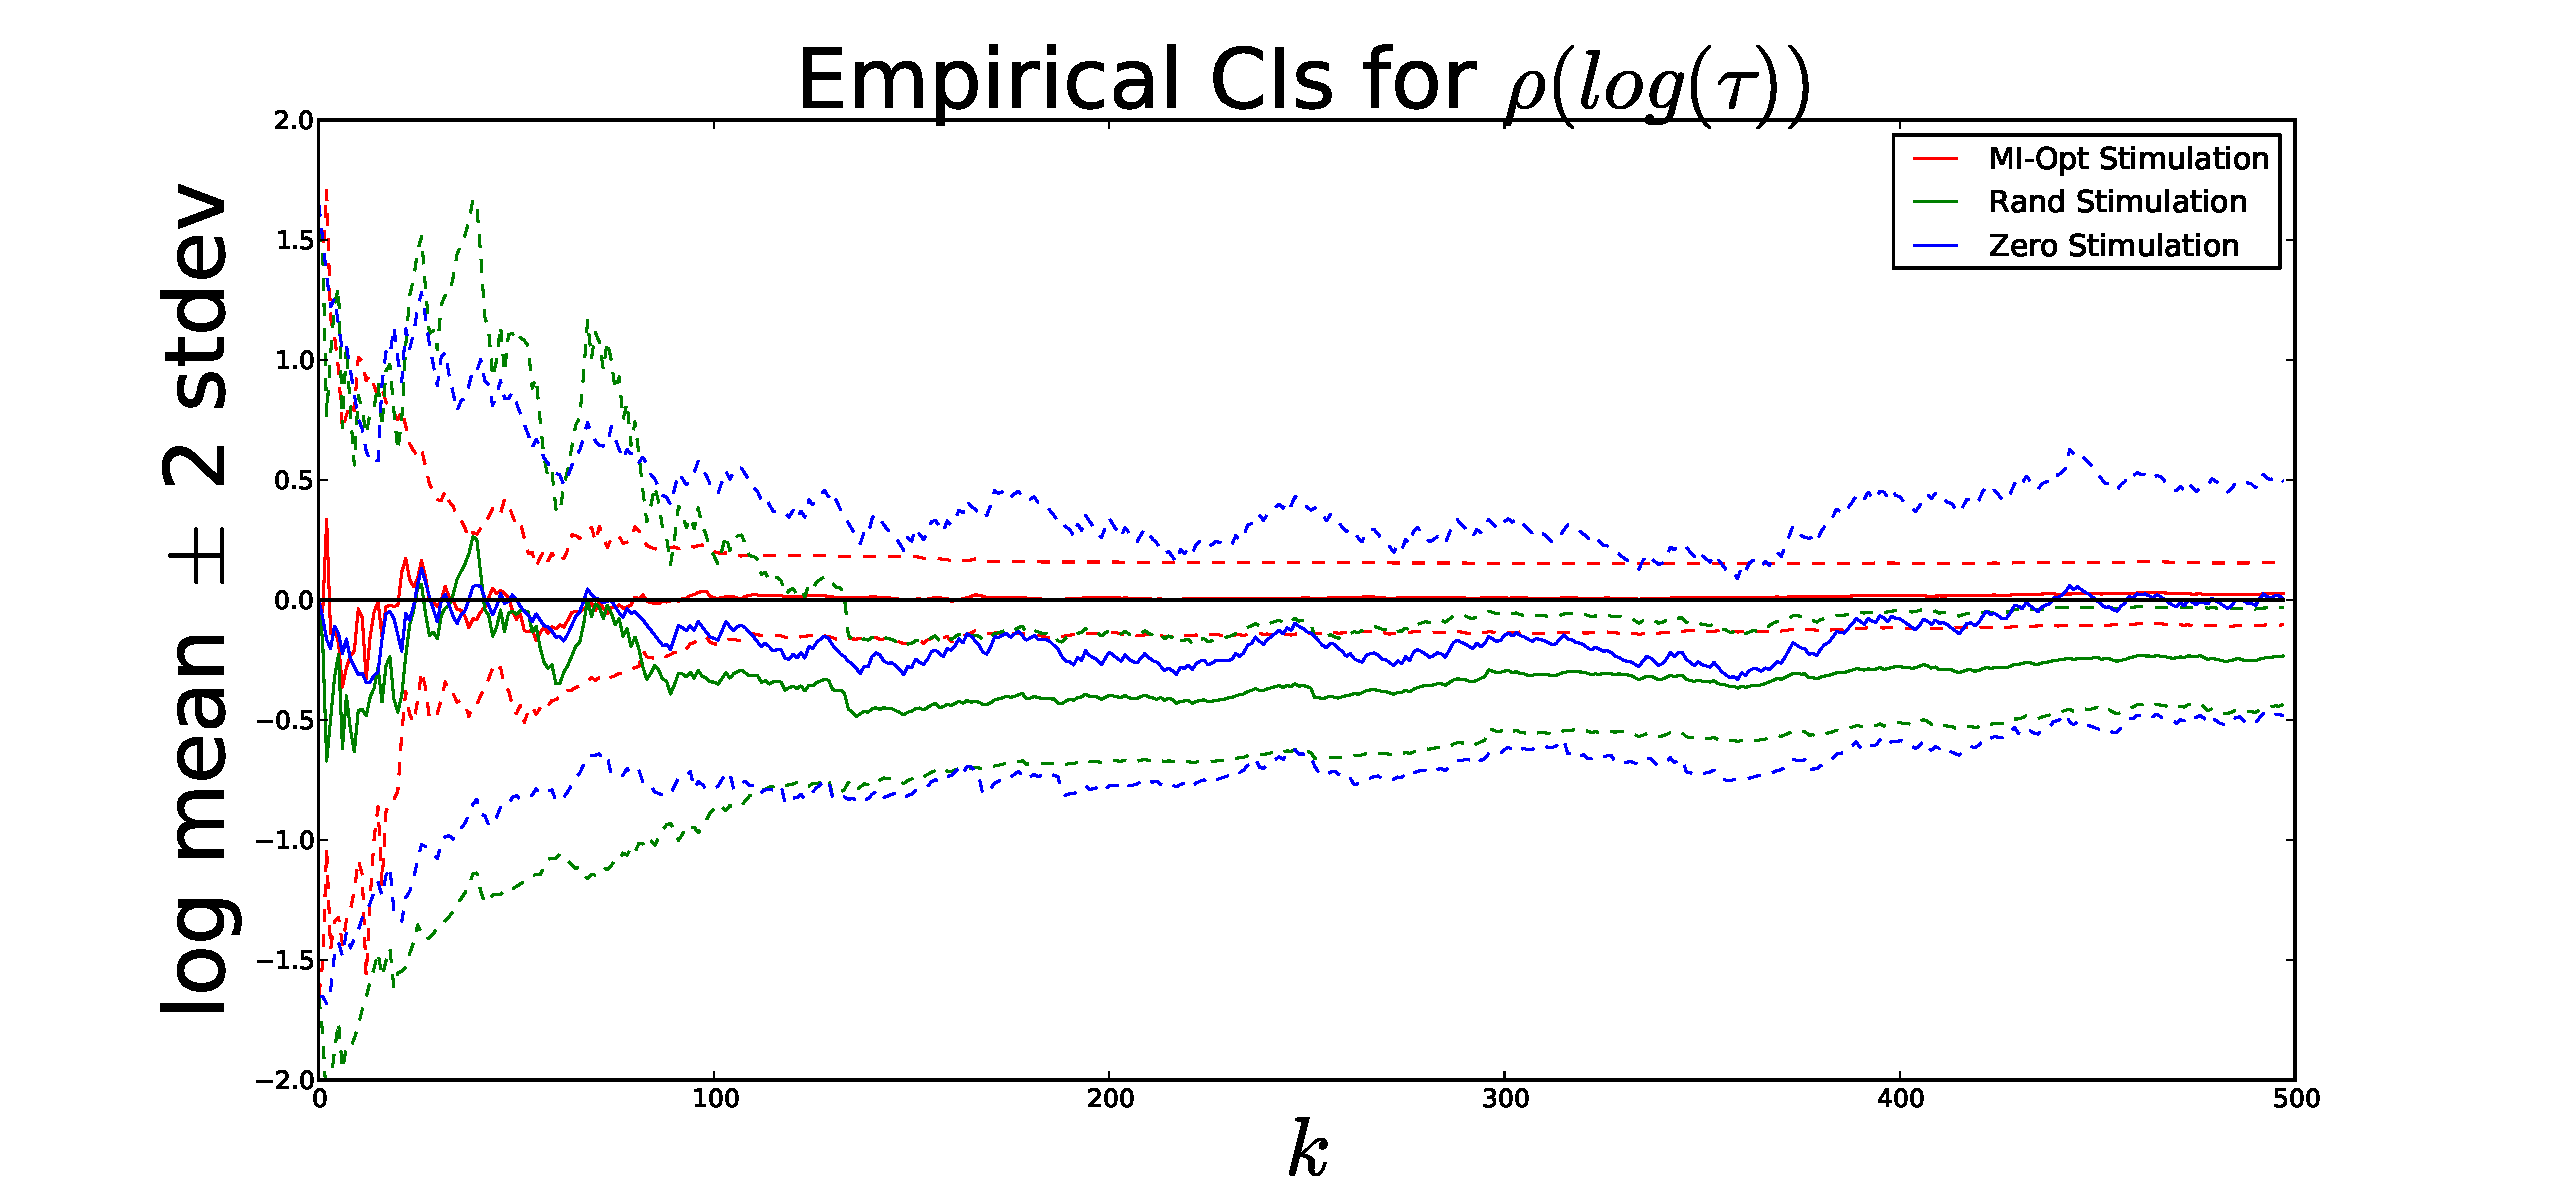
\includegraphics[width=0.48\textwidth]
{Figs/HTOnlineEstimator/single_experiment_exampleNts=32_Ntrls=497_ensemble_distn_evolution.pdf}
}
\subfloat[]
{
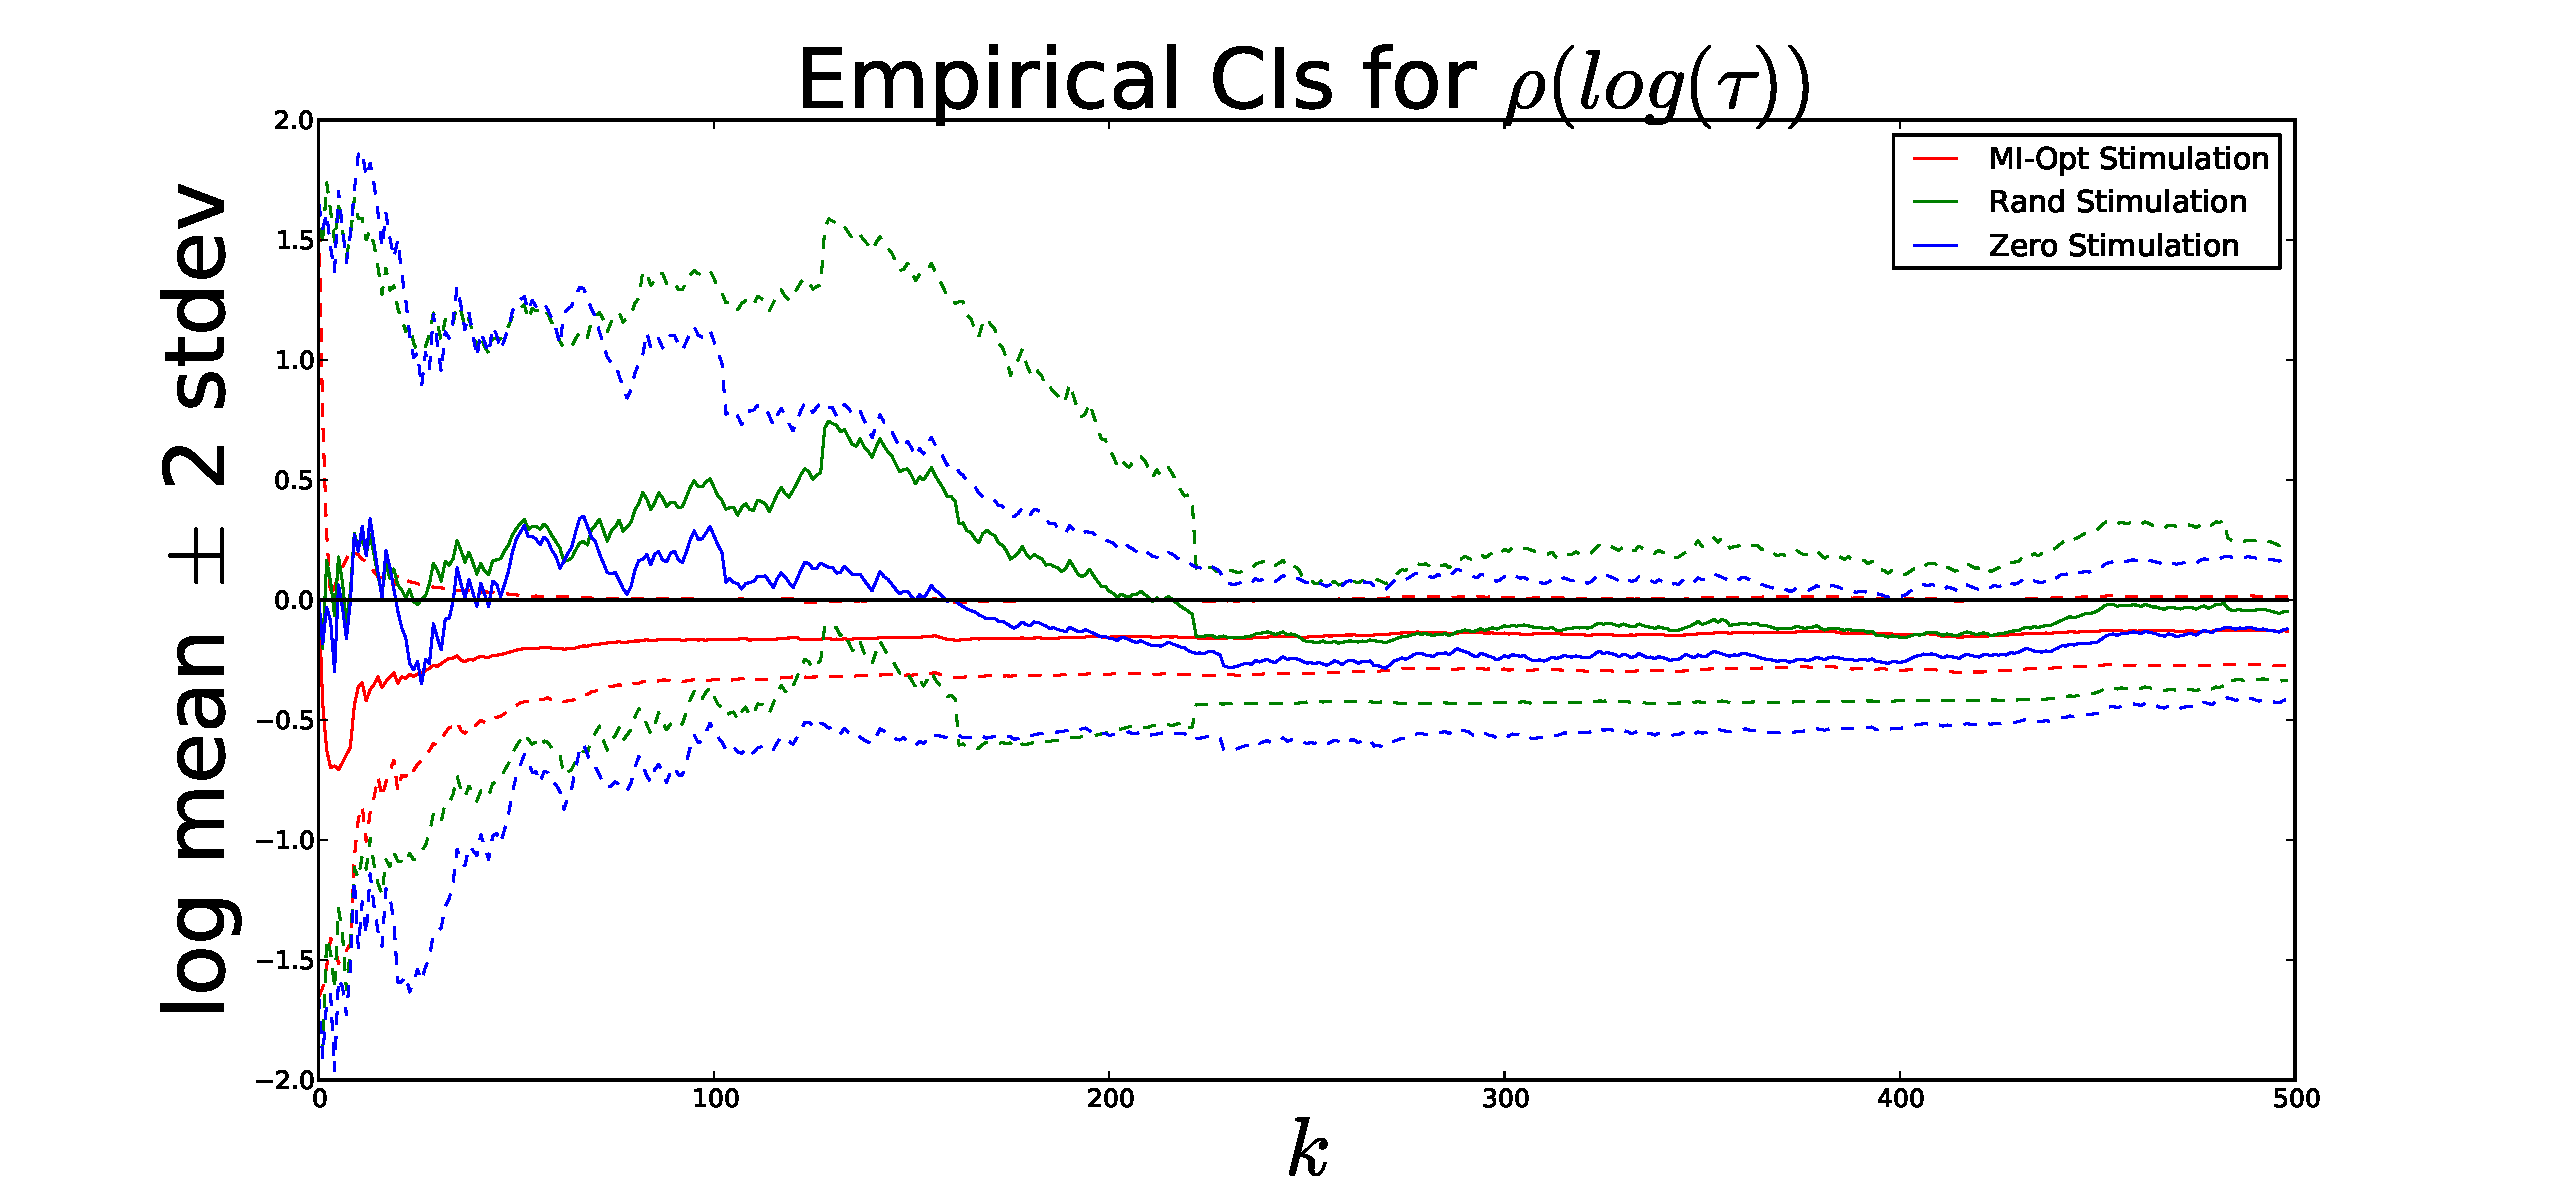
\includegraphics[width=0.48\textwidth]
{Figs/HTOnlineEstimator/single_experiment_exampleNts=32_Ntrls=498_ensemble_distn_evolution.pdf}
}\\
\subfloat[]
{
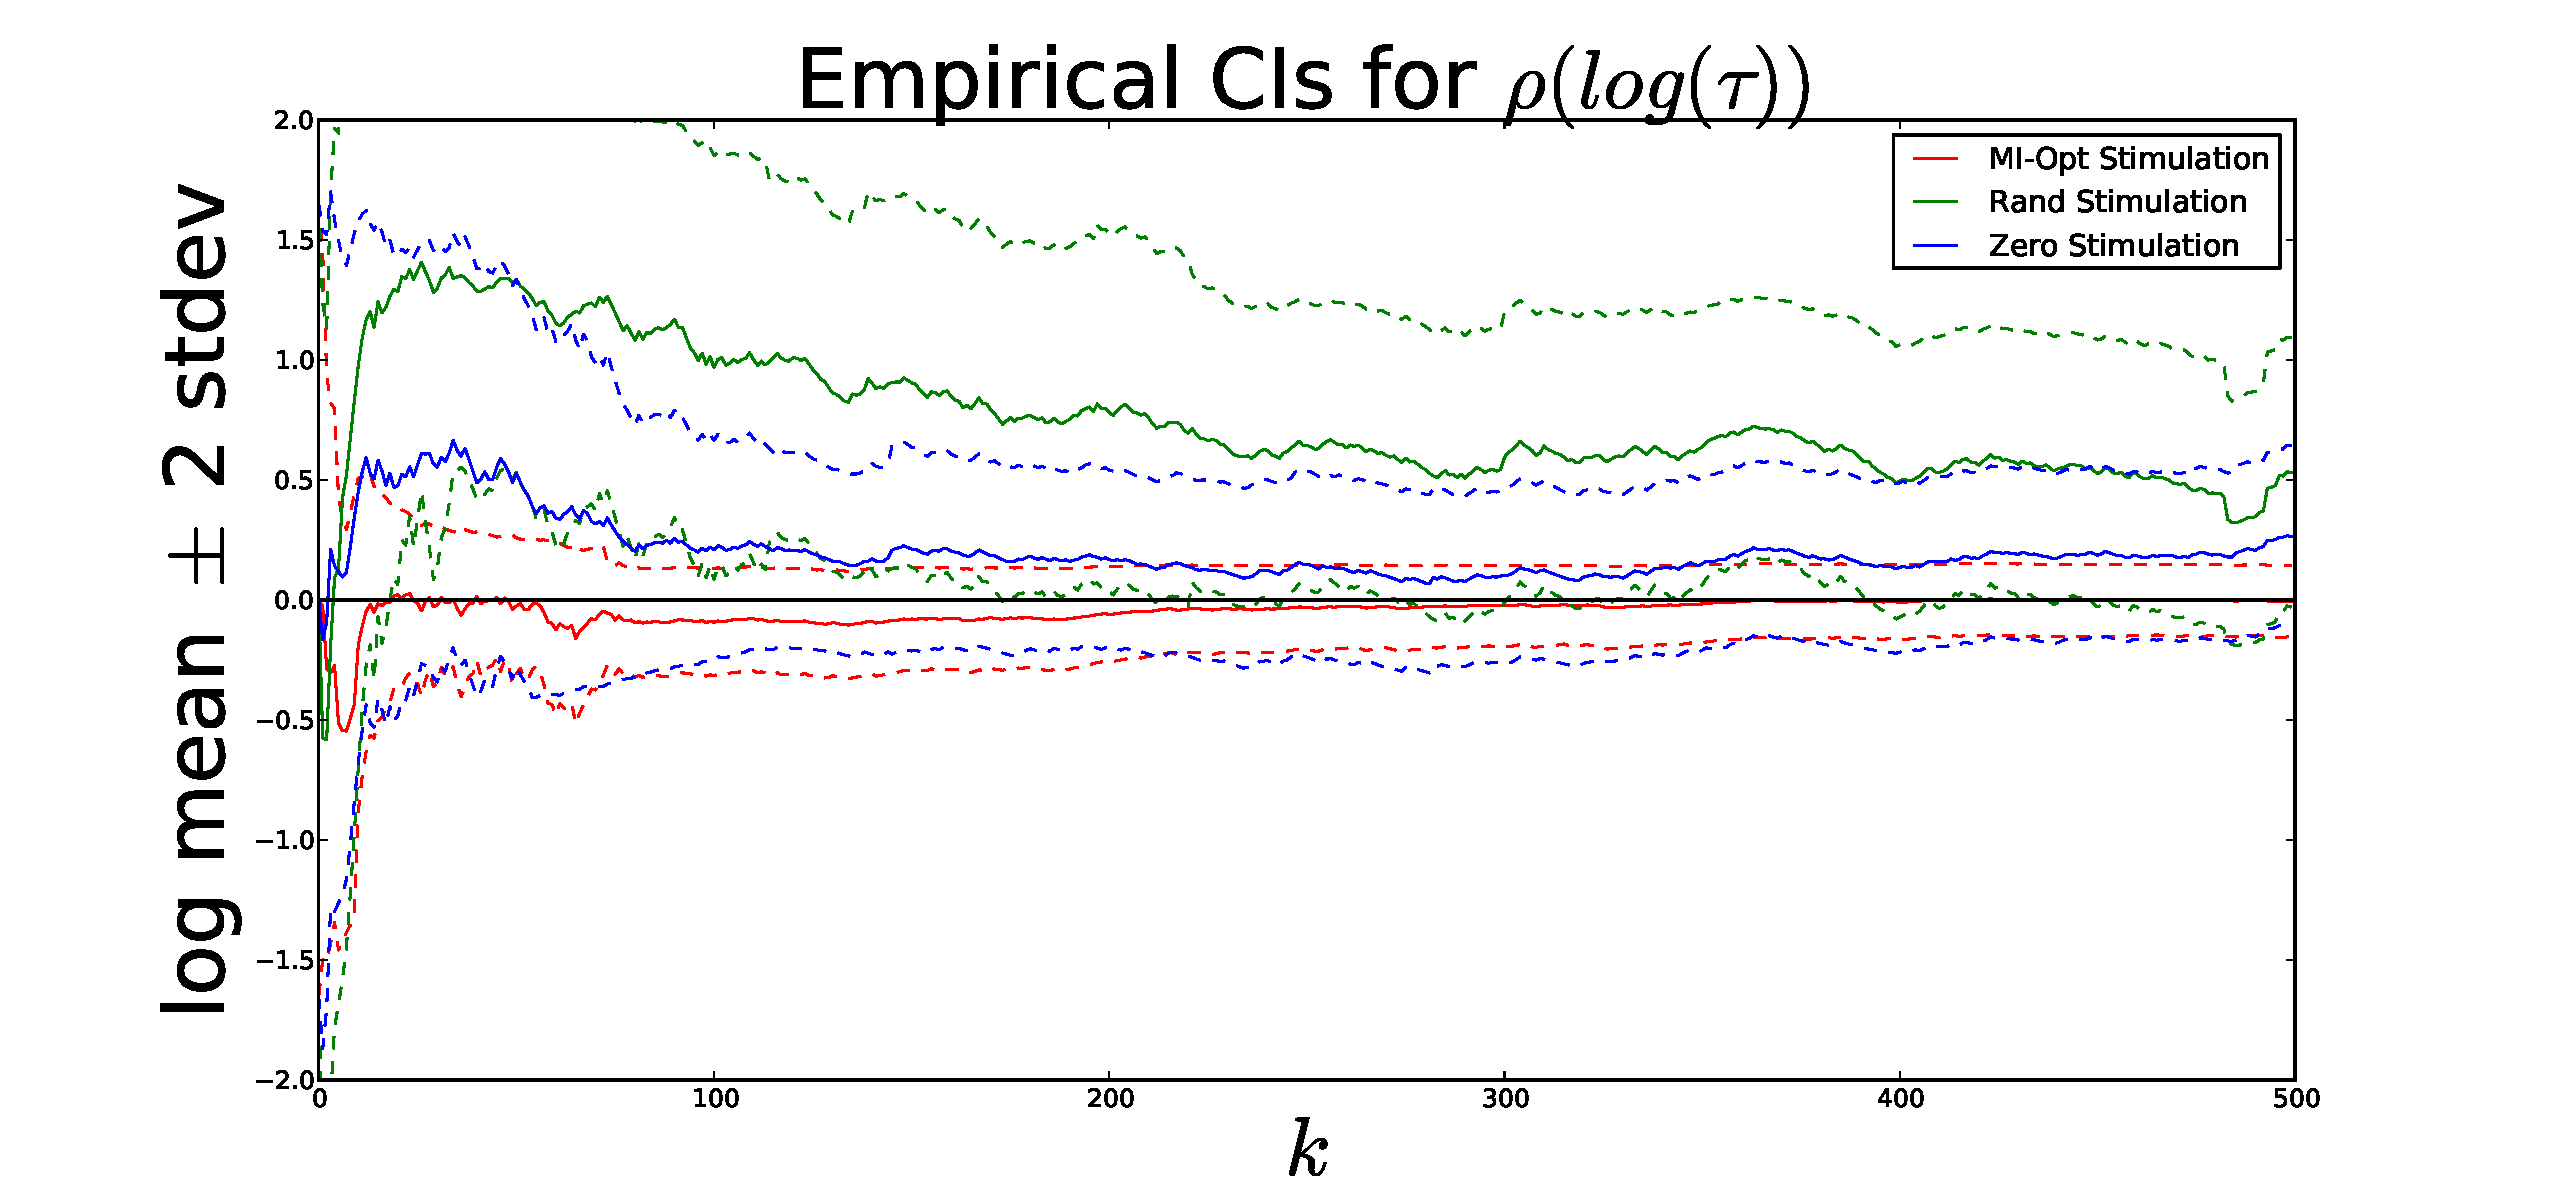
\includegraphics[width=0.48\textwidth]
{Figs/HTOnlineEstimator/single_experiment_exampleNts=32_Ntrls=499_ensemble_distn_evolution.pdf}
}
\subfloat[]
{
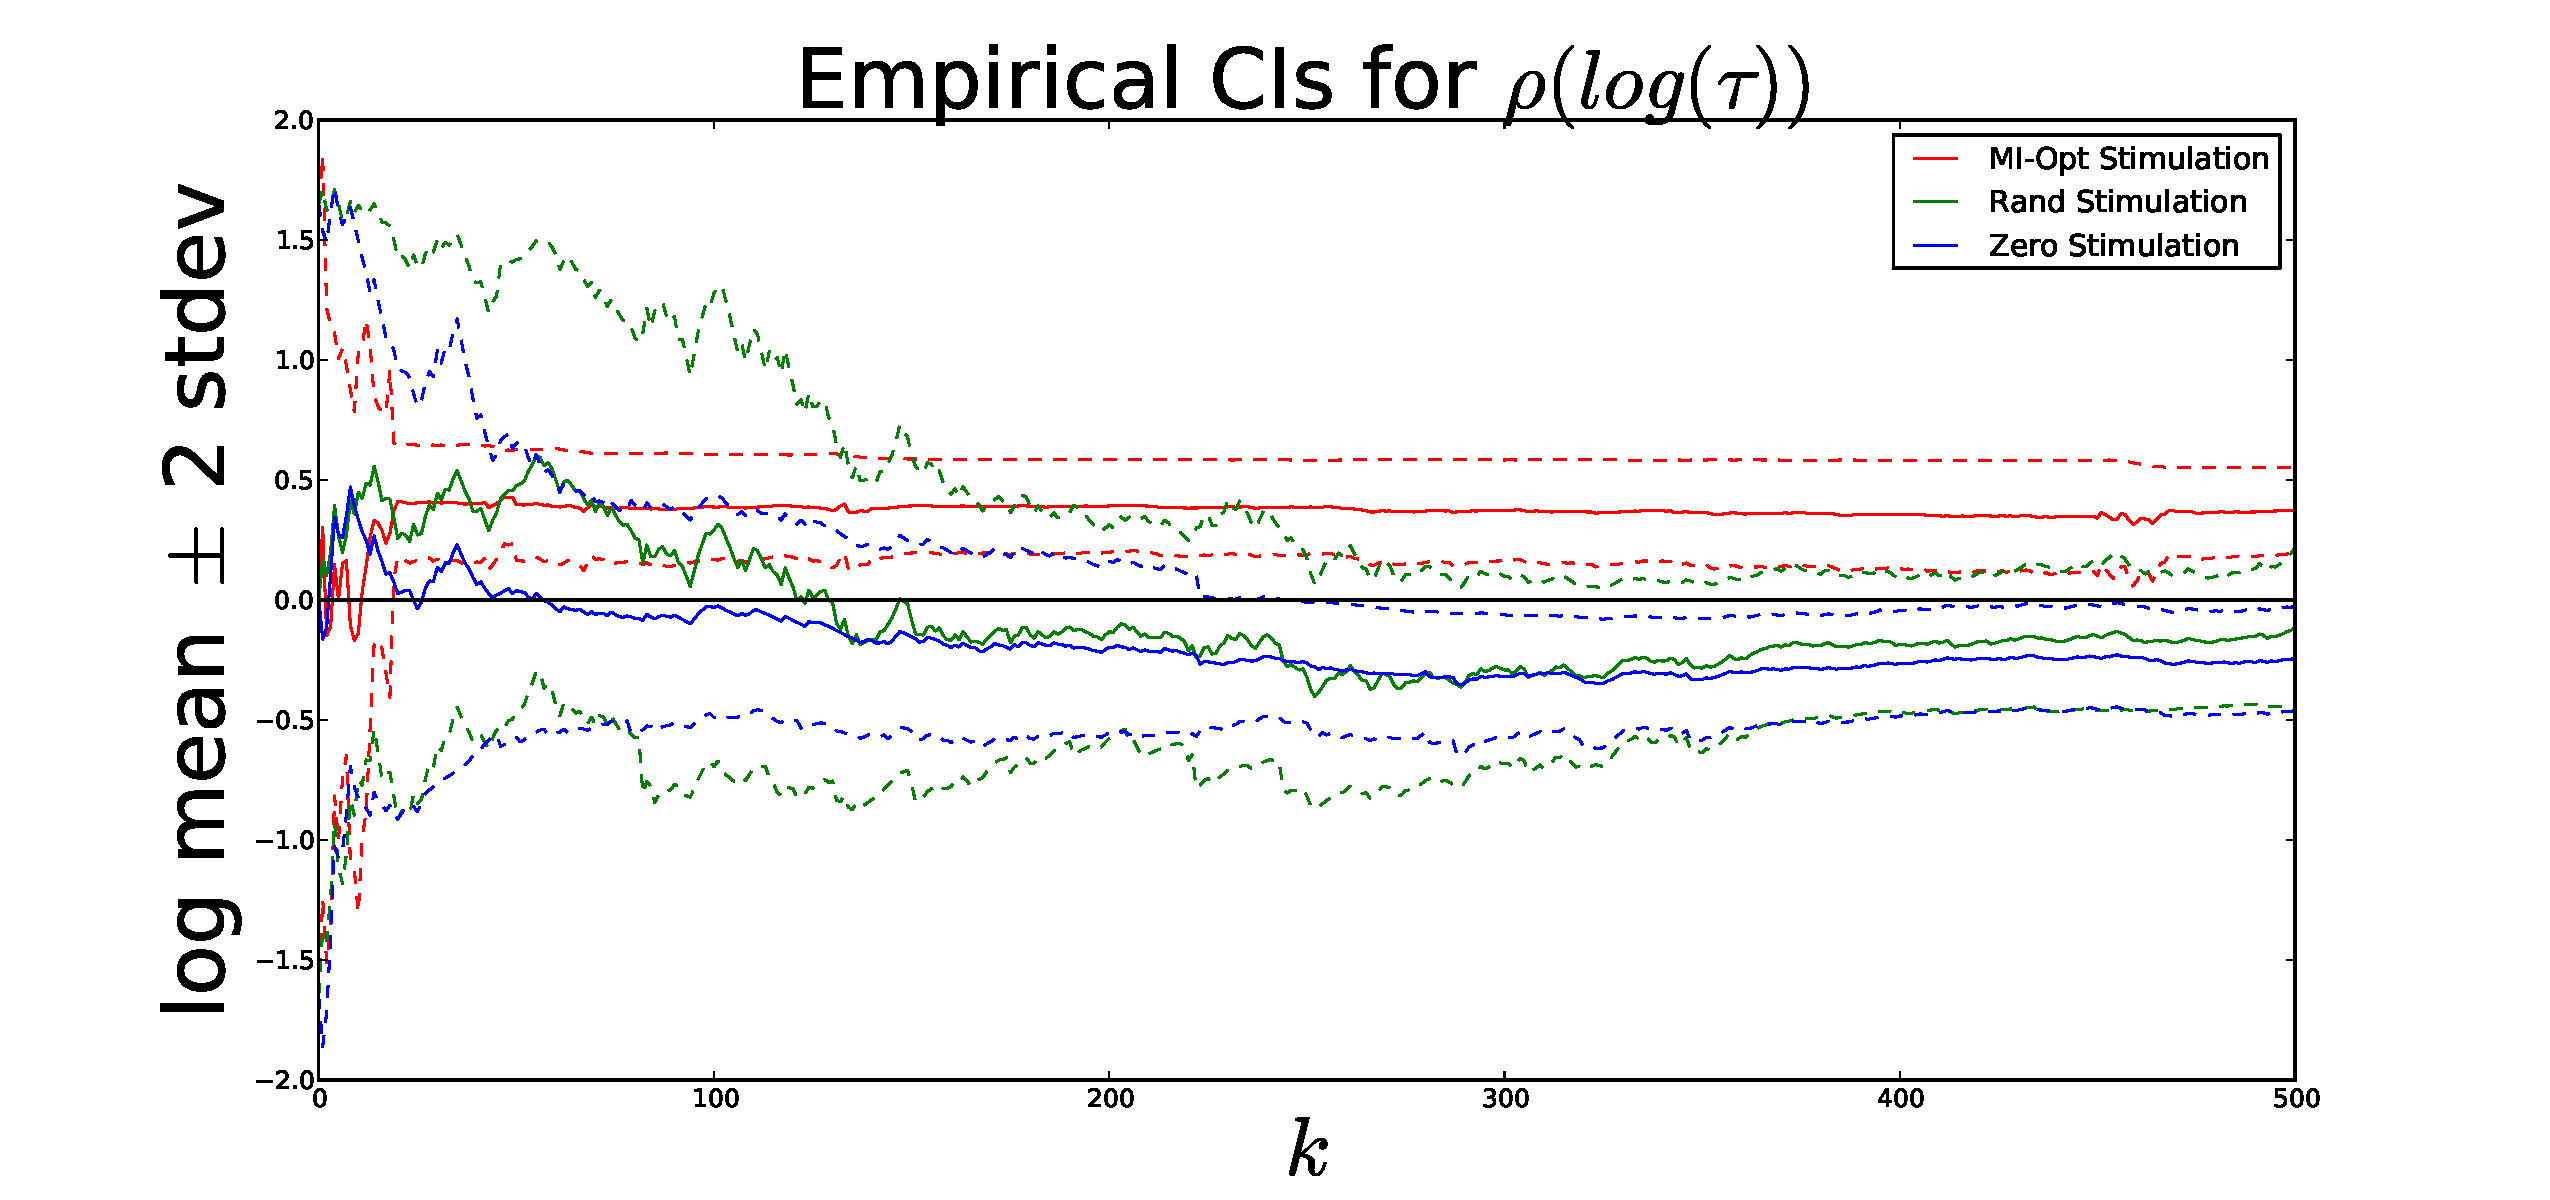
\includegraphics[width=0.48\textwidth]
{Figs/HTOnlineEstimator/single_experiment_exampleNts=32_Ntrls=500_ensemble_distn_evolution.pdf}
}\\
\subfloat[]
{
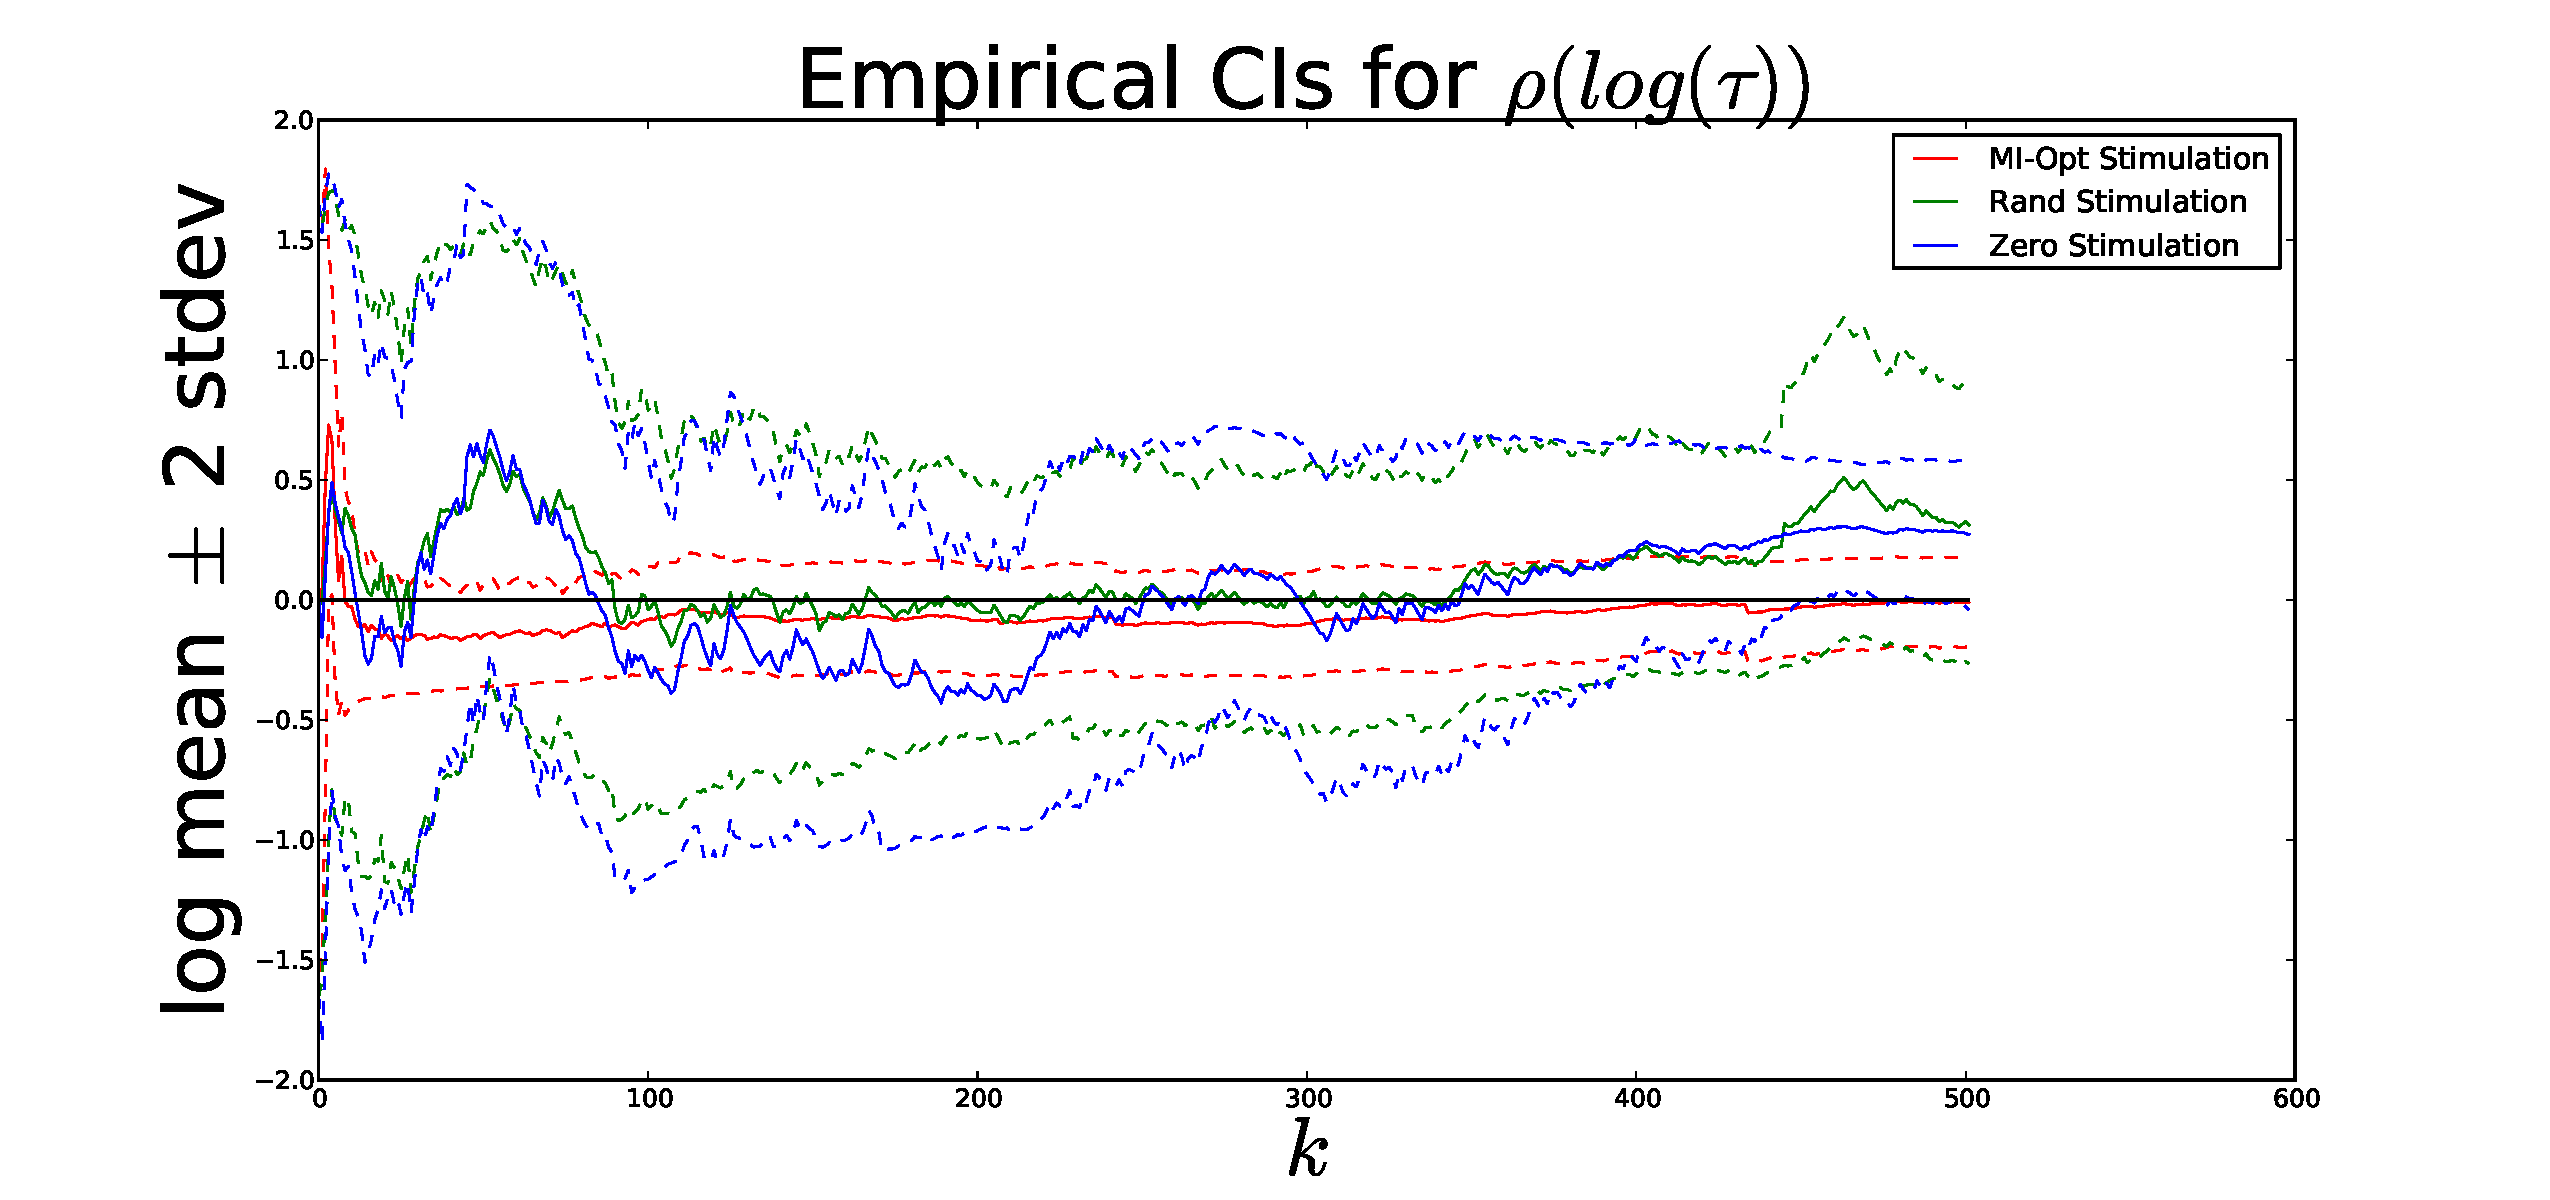
\includegraphics[width=0.48\textwidth]
{Figs/HTOnlineEstimator/single_experiment_exampleNts=32_Ntrls=501_ensemble_distn_evolution.pdf}
} 
\subfloat[]
{
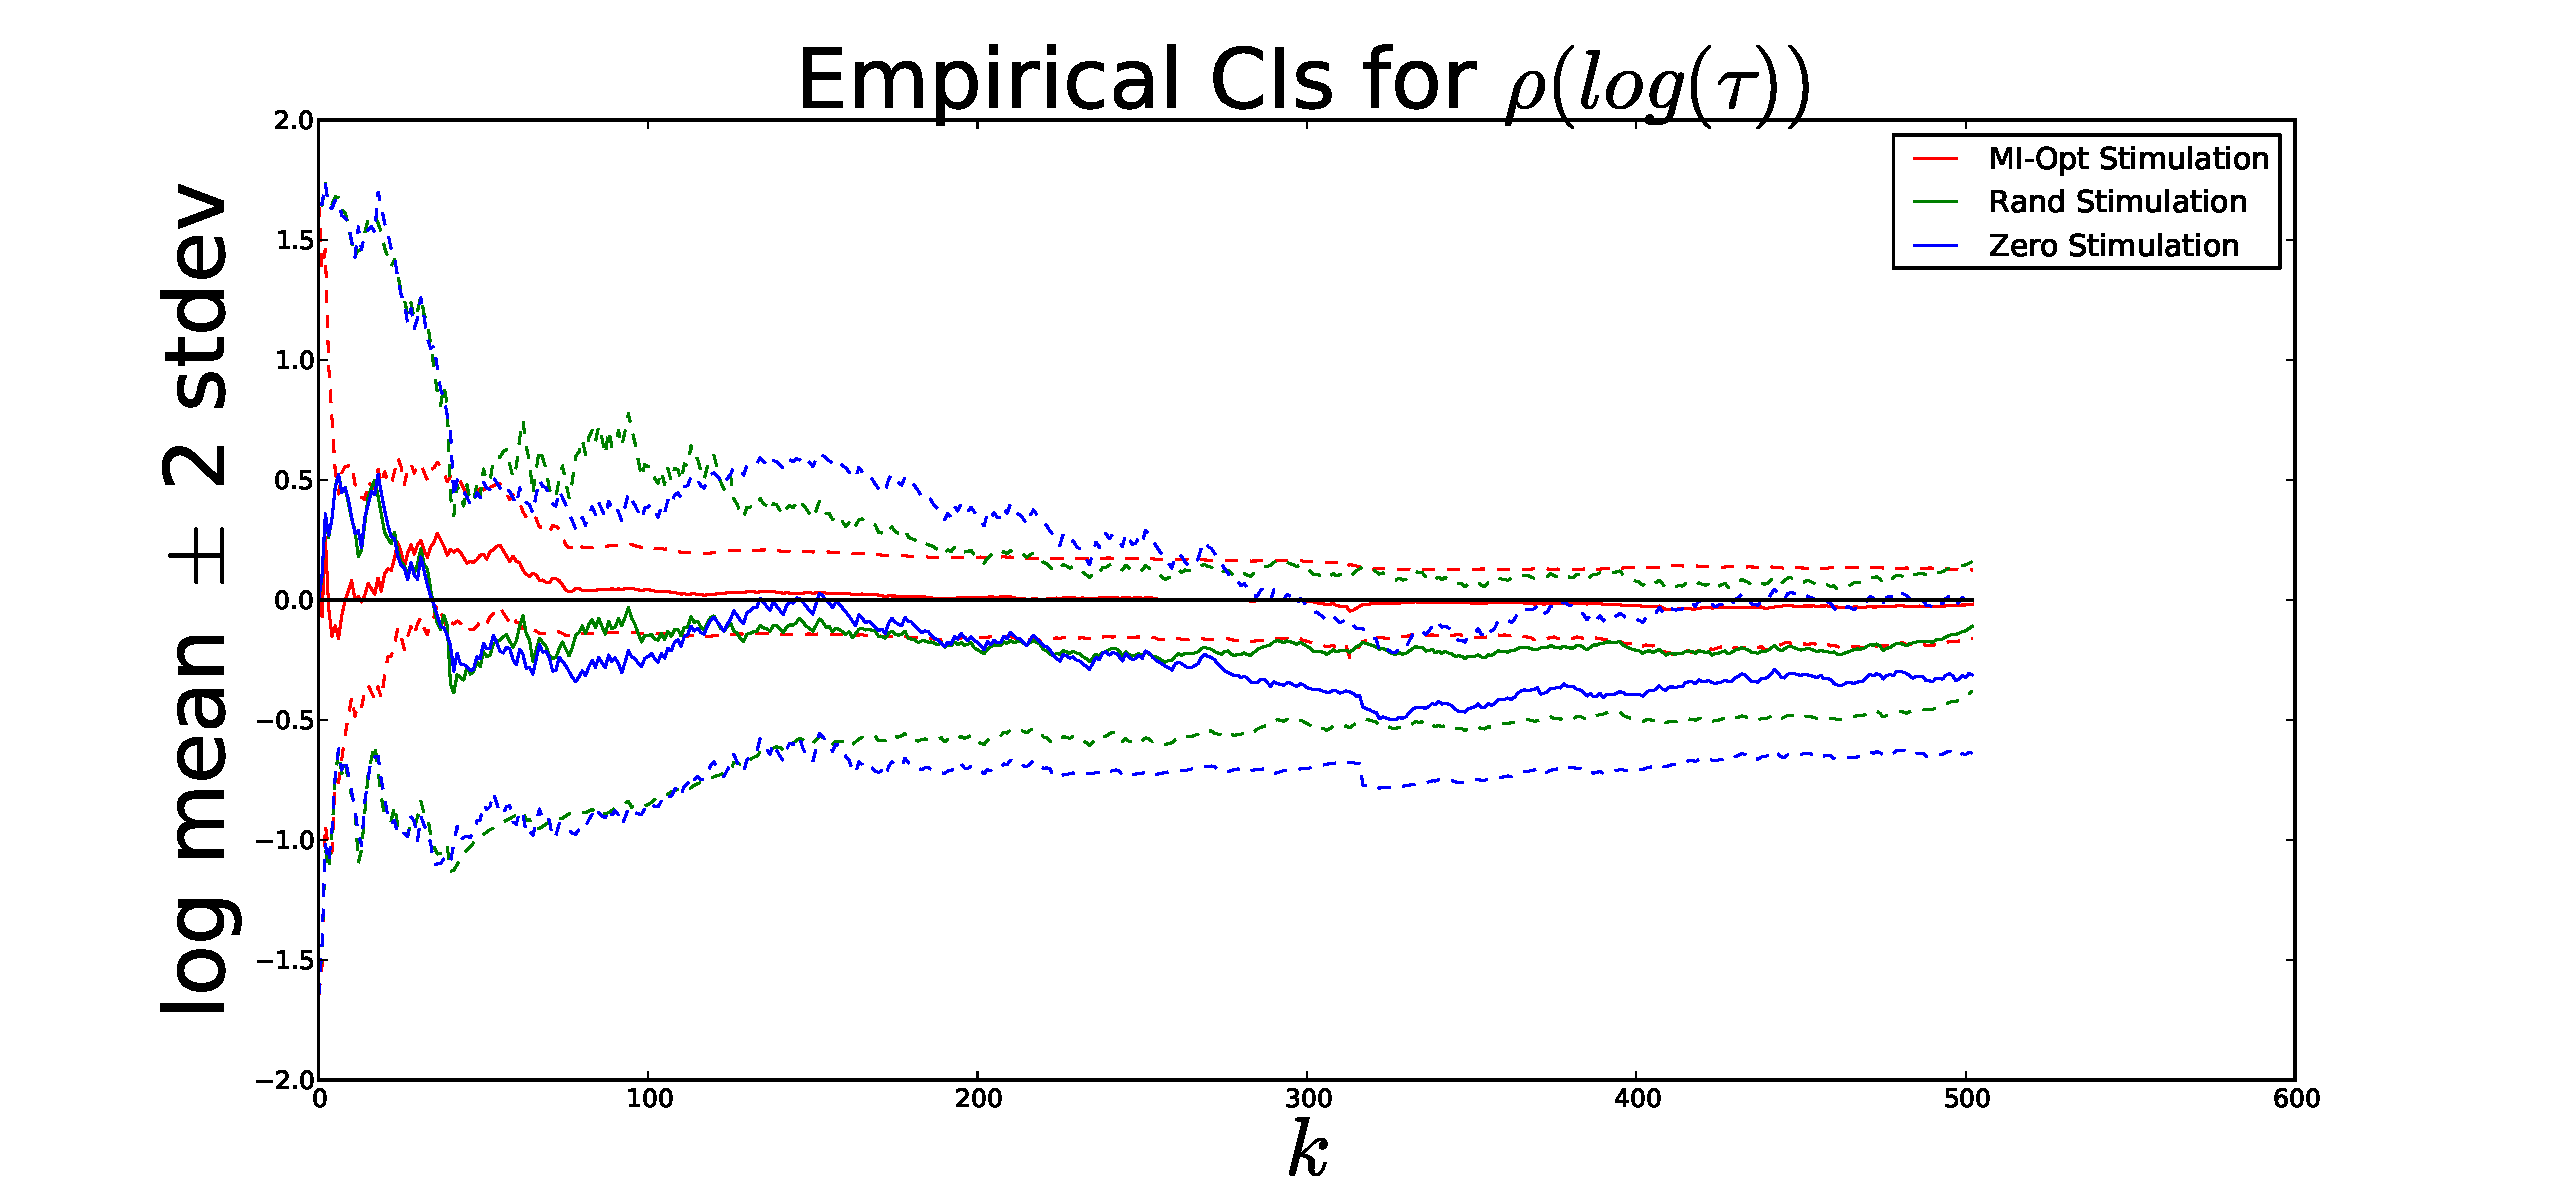
\includegraphics[width=0.48\textwidth] 
{Figs/HTOnlineEstimator/single_experiment_exampleNts=32_Ntrls=502_ensemble_distn_evolution.pdf}
}\\
\subfloat[]
{
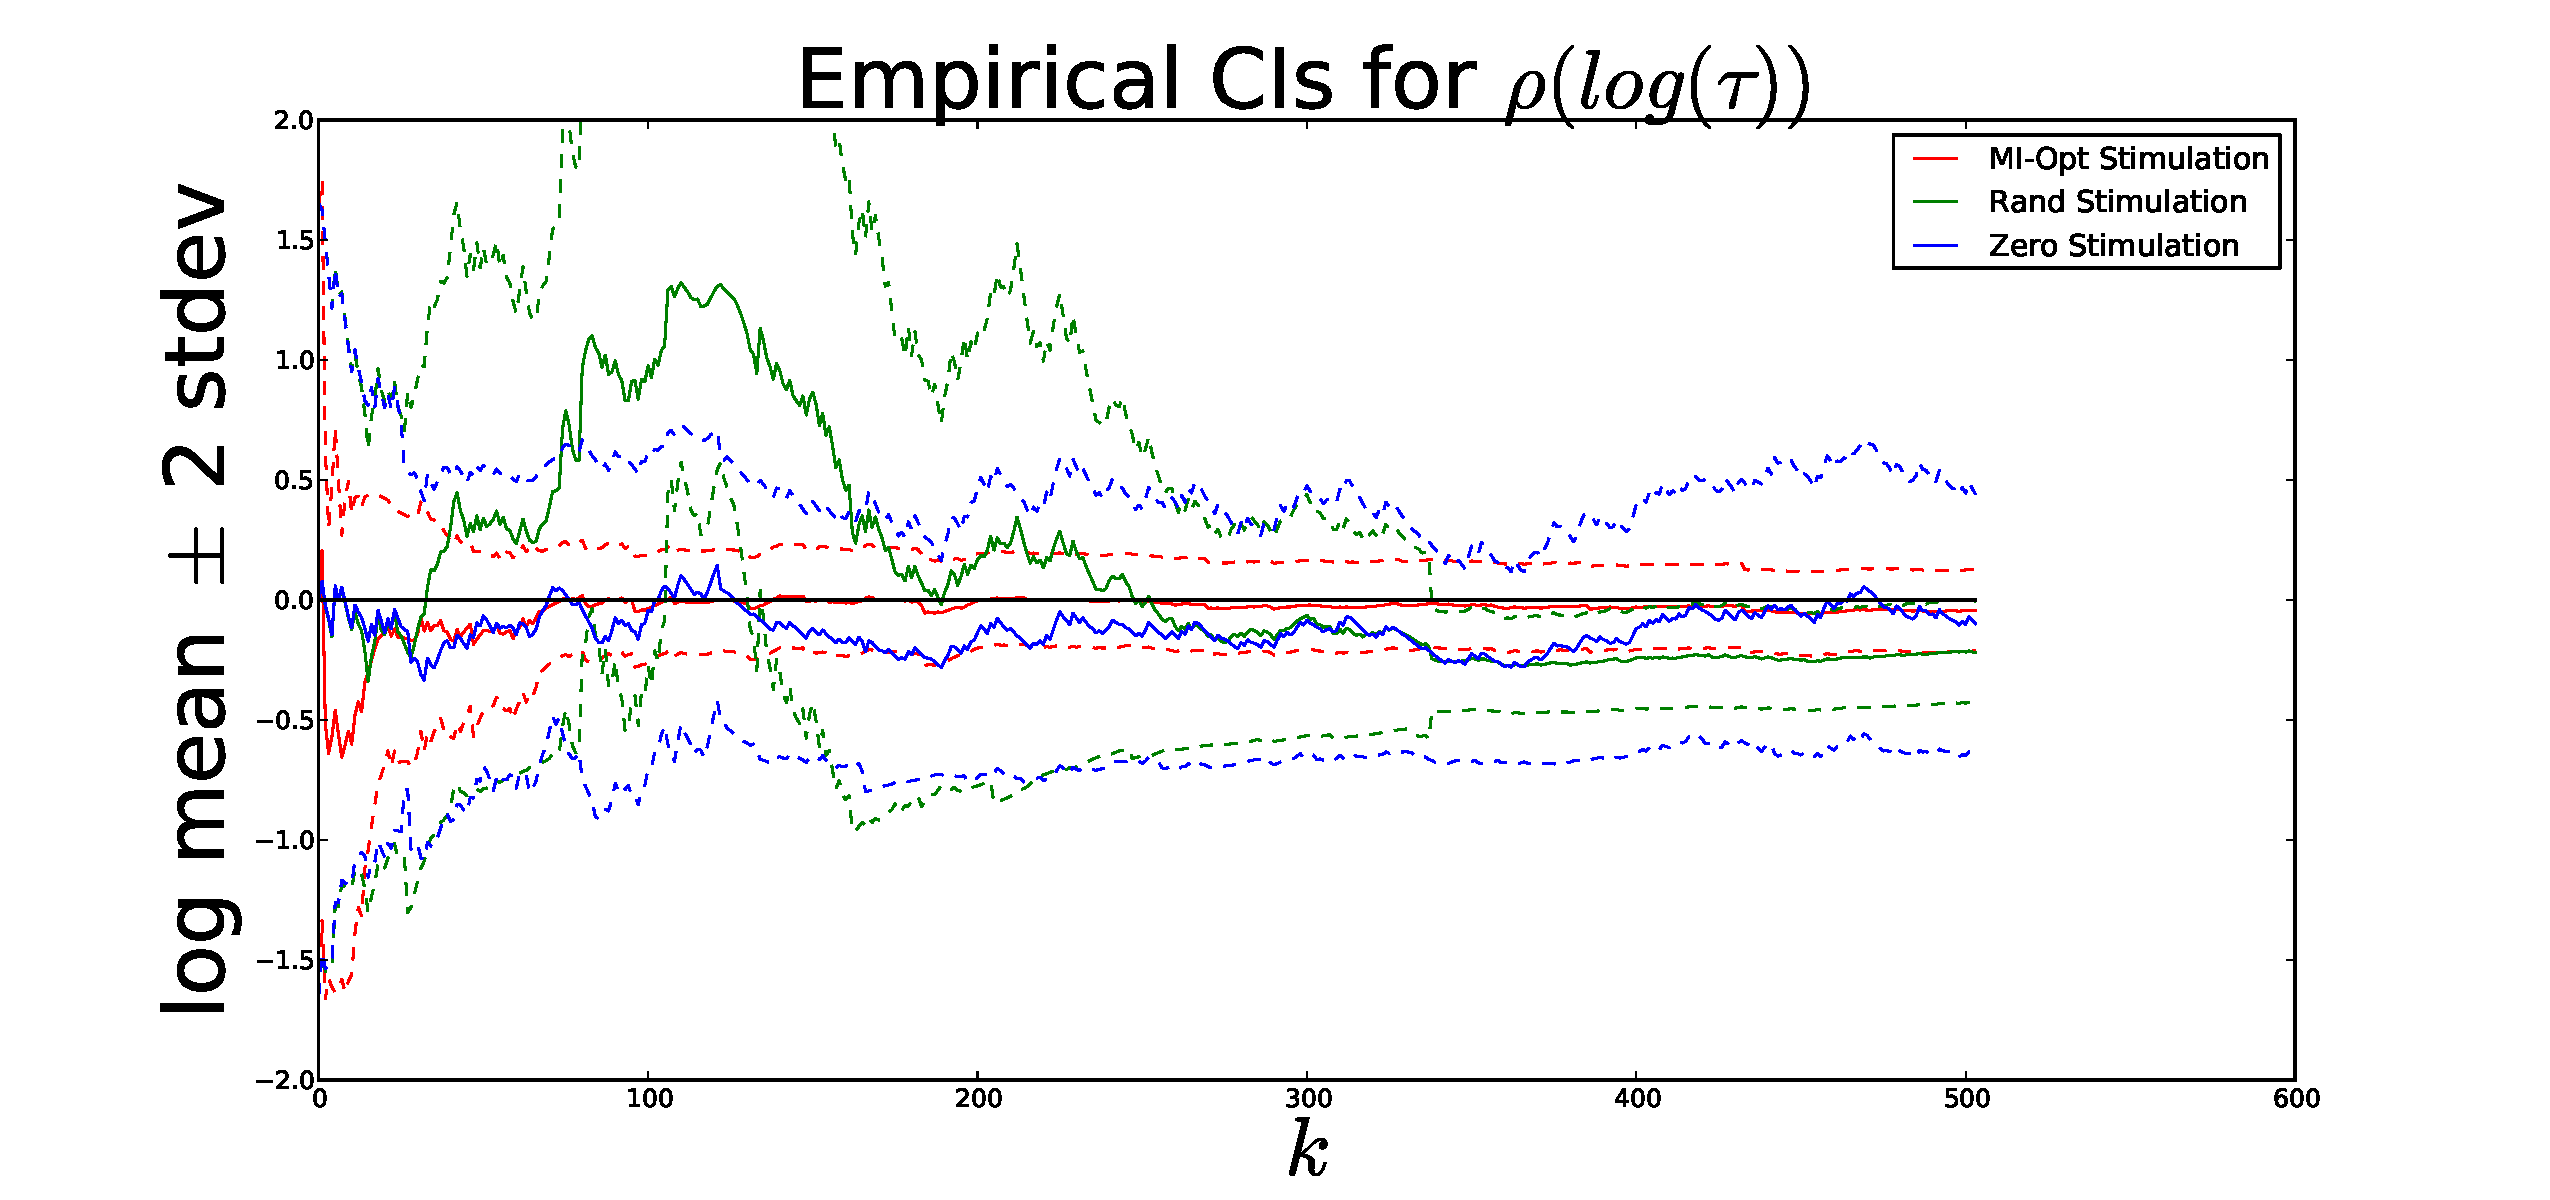
\includegraphics[width=0.48\textwidth]
{Figs/HTOnlineEstimator/single_experiment_exampleNts=32_Ntrls=503_ensemble_distn_evolution.pdf}
}
\subfloat[] 
{
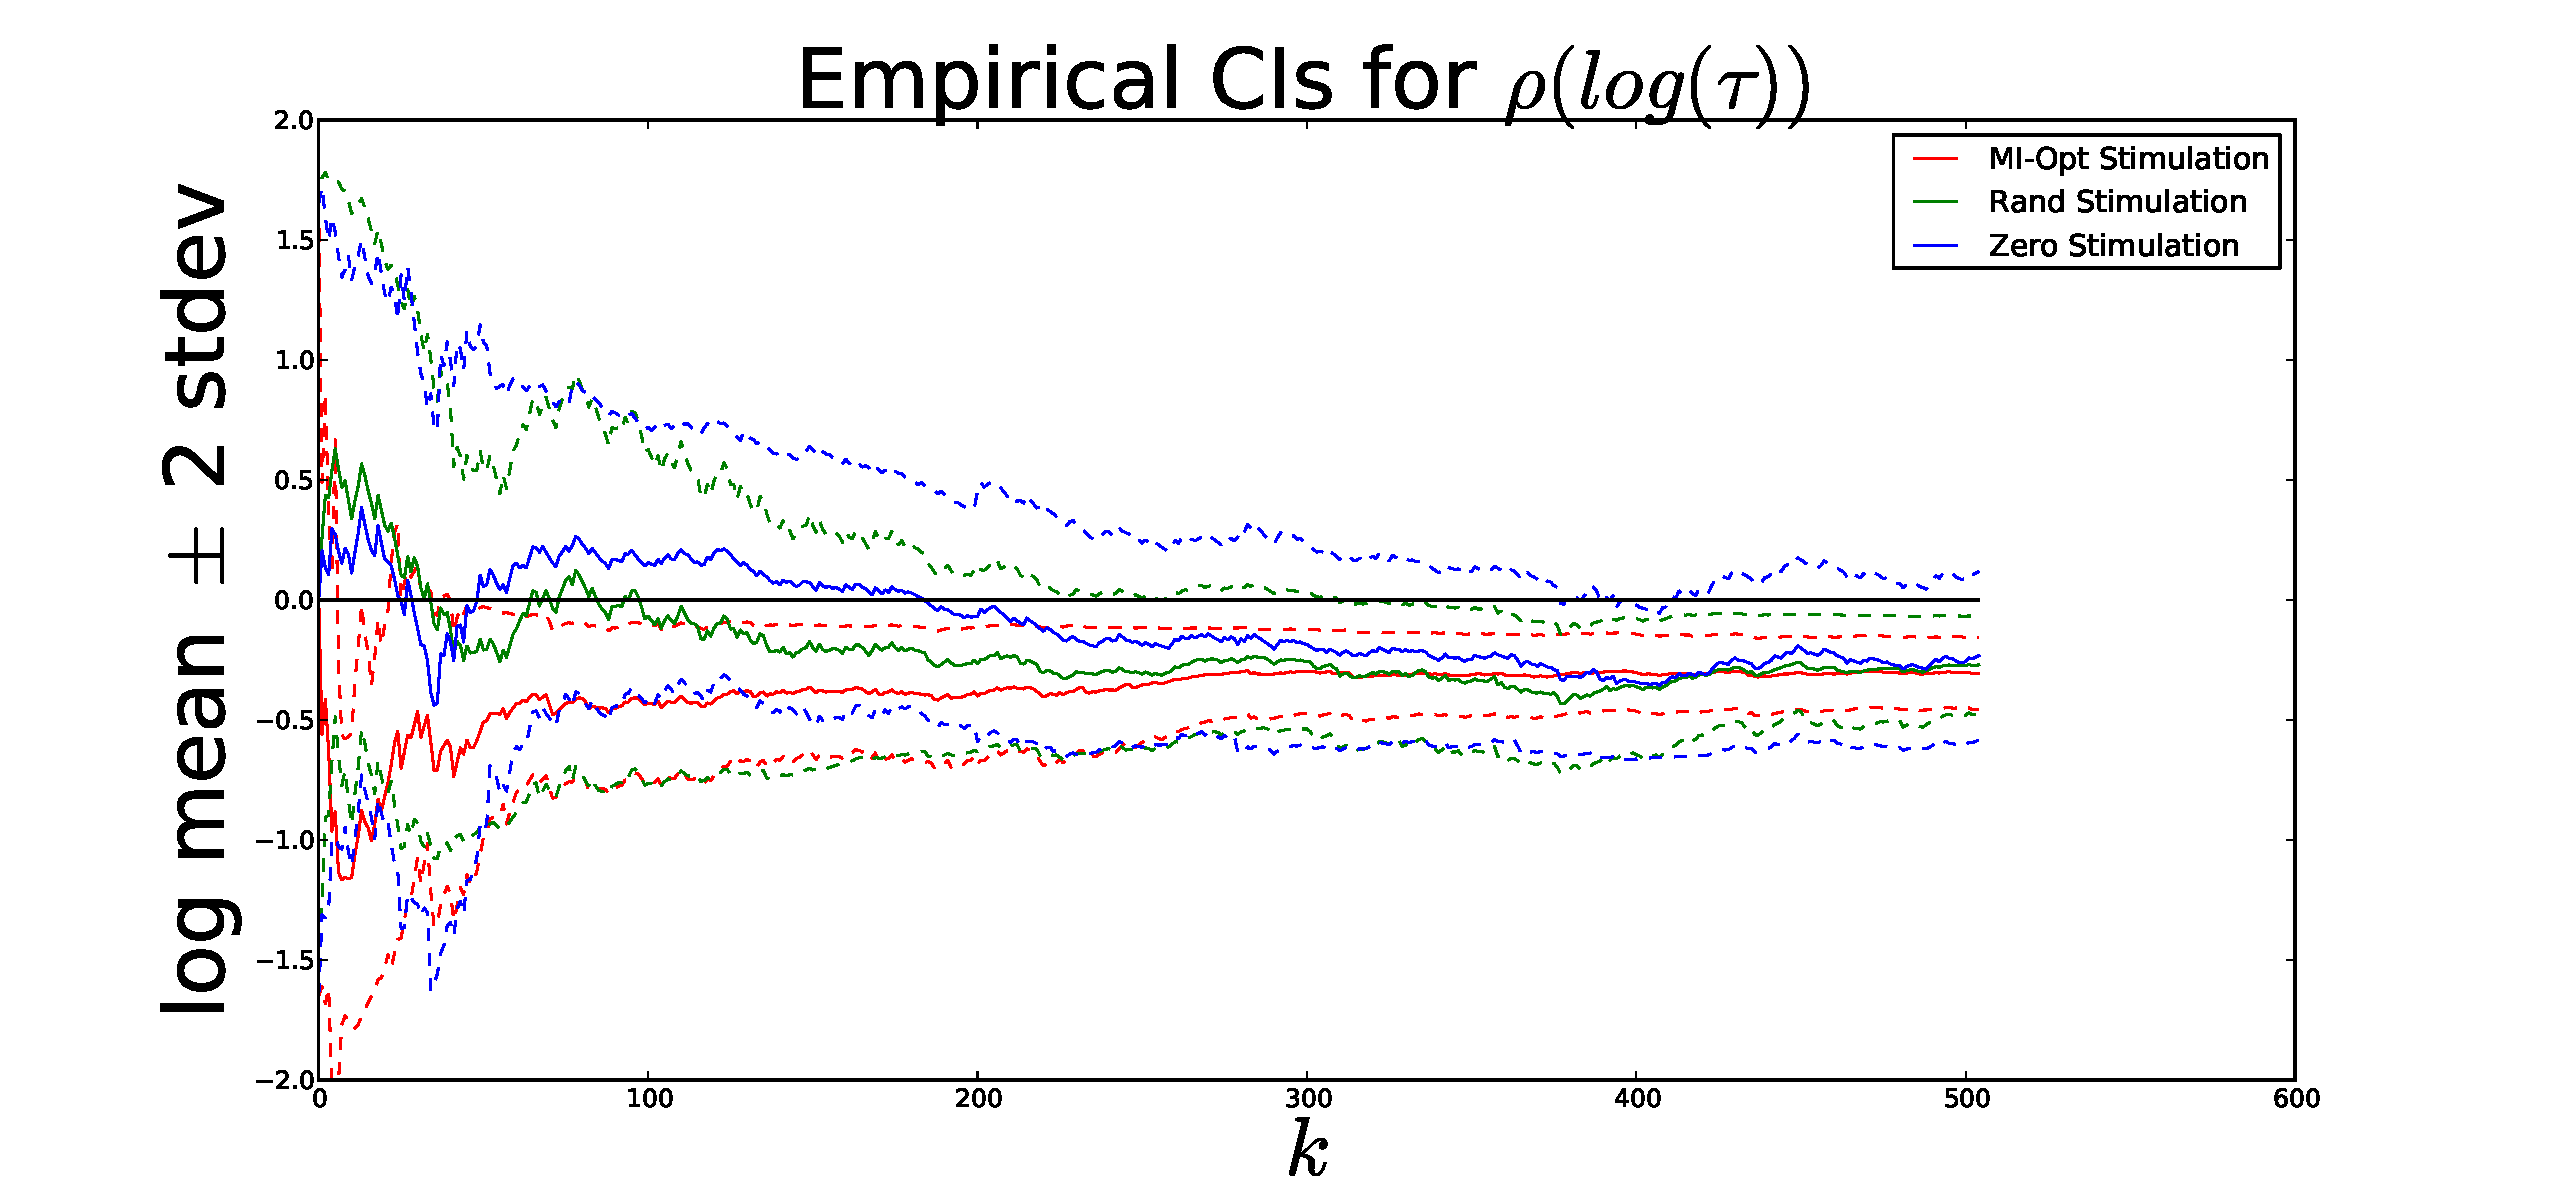
\includegraphics[width=0.48\textwidth]
{Figs/HTOnlineEstimator/single_experiment_exampleNts=32_Ntrls=504_ensemble_distn_evolution.pdf}
}
\caption[labelInTOC]{Various examples of the perturbation-estimation protocol
with the belief distribution plotted against the hitting time $k$,  with the
MI-optimal stimulation (red), the constant random stimulation (green) and the zero, $\a\equiv 0\,\forall t$, stimulation (blue)}
\label{fig:online_optimization_more_examples}
\end{center}
\end{figure} 

The aggregated version of these results (the averaged evolution distribution
from the independent experiments) is shown
\cref{fig:online_optimization_aggregated_belief_evolution}, where the $N$
distributions are averaged out over the different experiments. It is now clear 
that the MI-Optimal procedure produces more accurate estimates much faster.
 
% \usepackage{graphics} is needed for \includegraphics
\begin{figure}[htp]
\begin{center}
  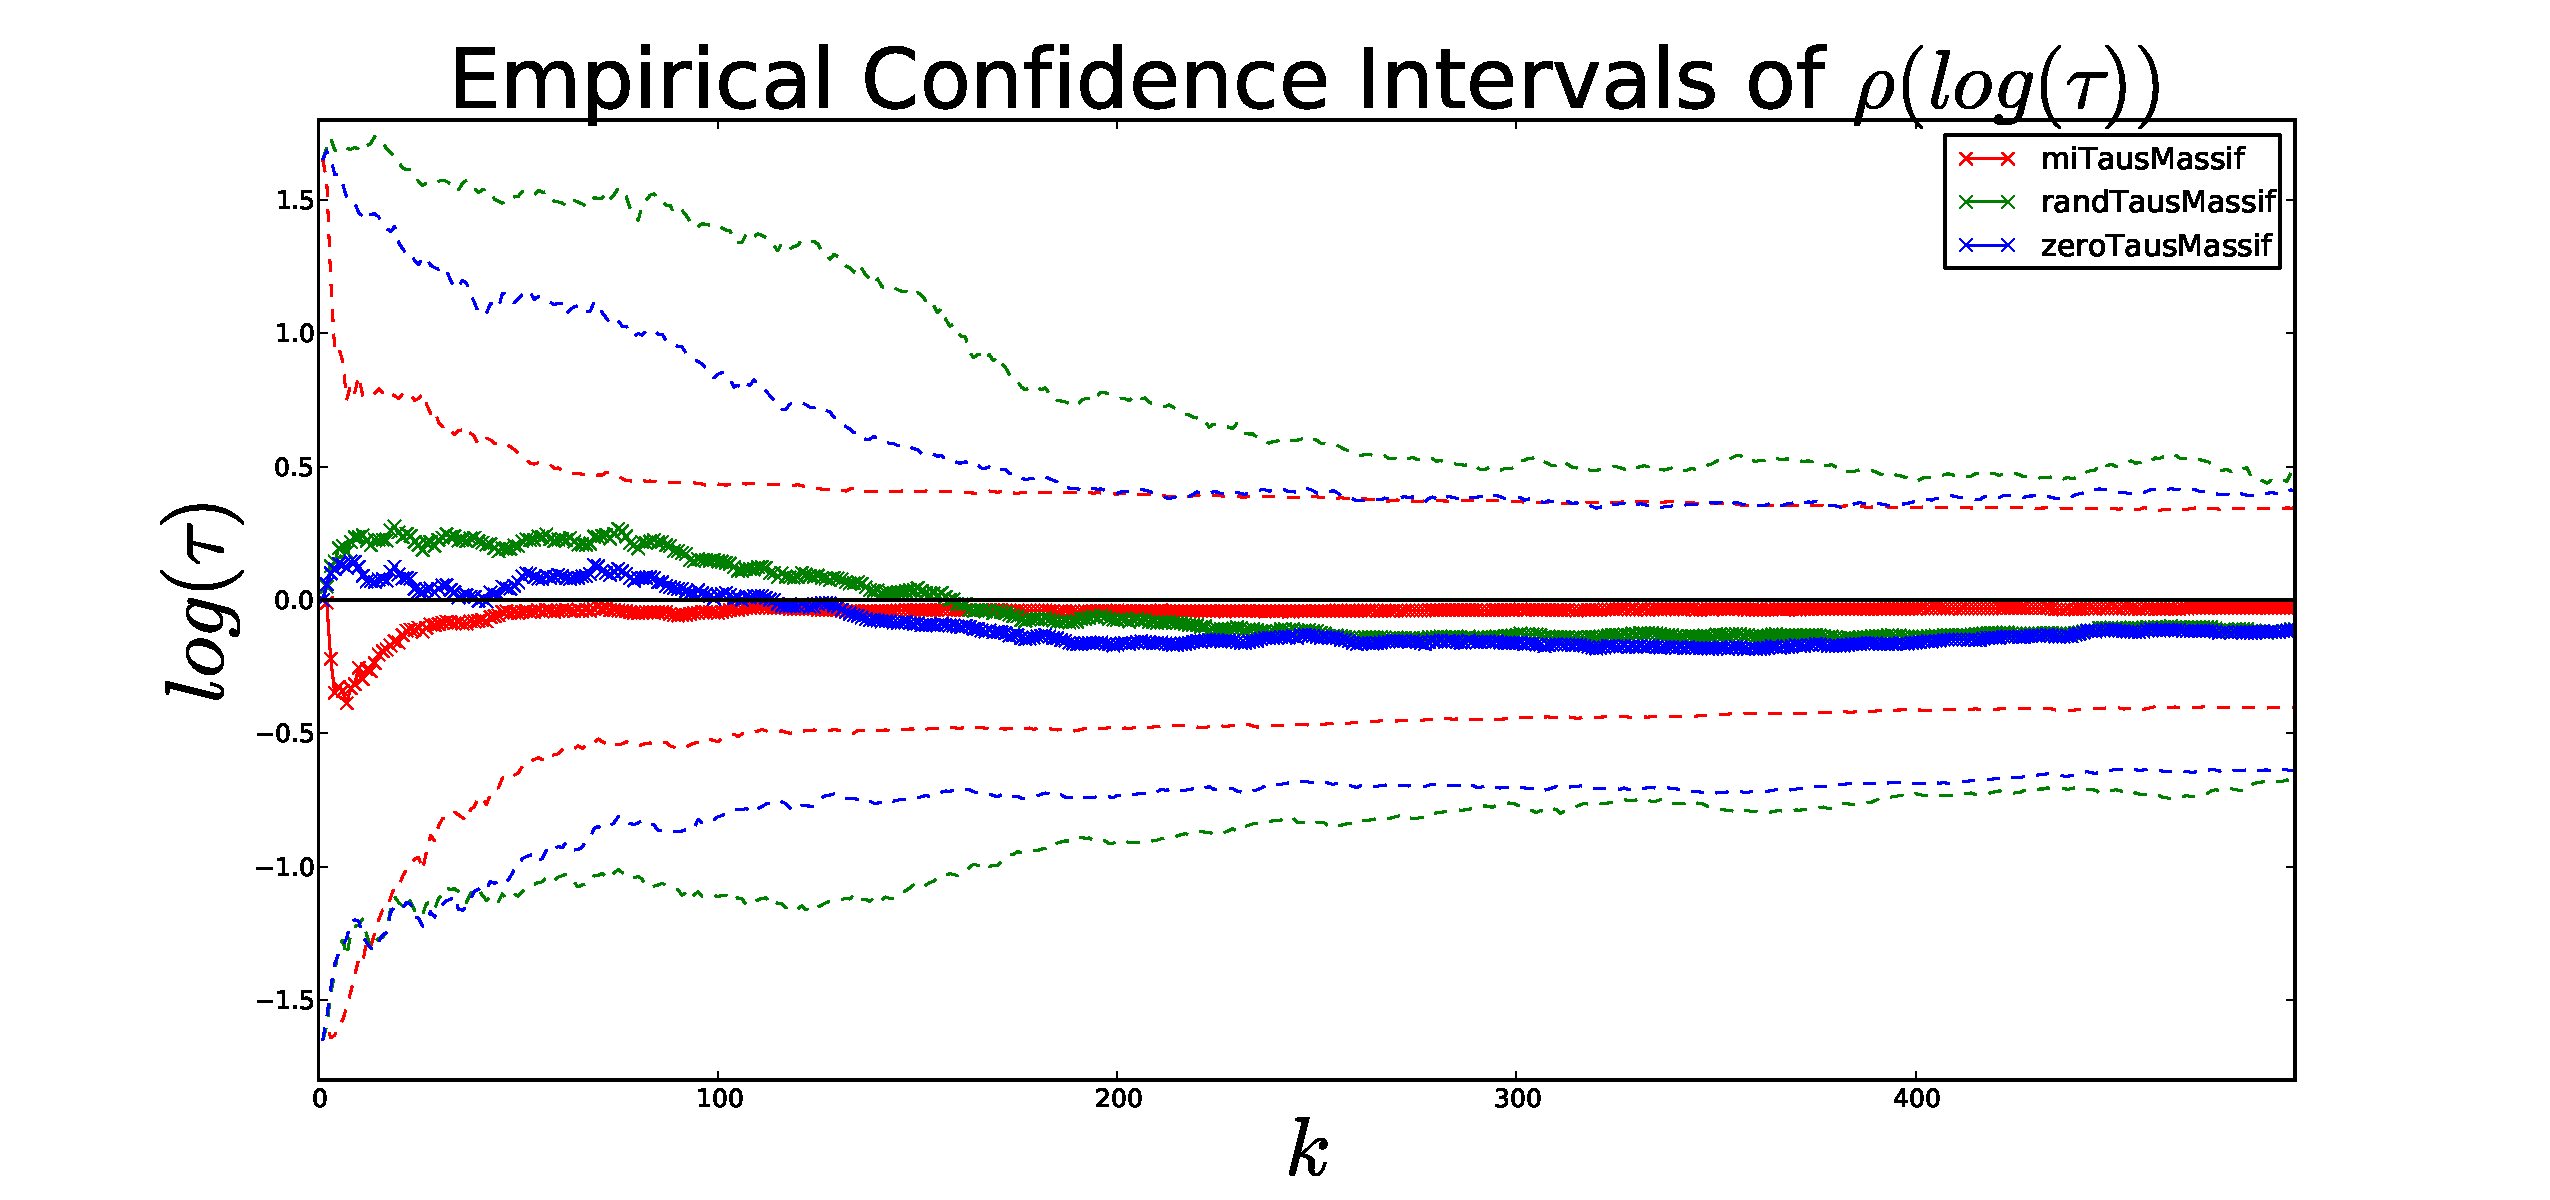
\includegraphics[width=\textwidth]{Figs/HTOnlineEstimator/aggregated_belief_distn_aggregated_ensemble_distn_evolution.pdf}
  \caption[Aggregated belief distribution vs. experiment hitting time index]{Aggregated belief distribution over $N=16$ independent belief estimation experiment. The black line indicates the 'true' value of the
  unknown parameter $\tau$. } 
  \label{fig:online_optimization_aggregated_belief_evolution}
\end{center}
\end{figure}




\clearpage













\appendix
\section{The basic idea of optimal design for SDEs of Lin et al.}
Here we sketch the basic idea of Lin et al. \cite{Lin}. 

Let us write the dynamics as such
\begin{equation}
dX = \underbrace{f(X,\th, \a)}_{\textrm{controlled drift}}dt
+ \b dW
\end{equation}
Then given an observed path $\{x_t\}_0^\tf$, the log-likelihood, $l$ wrt.\ the
parameter set $\th$ is
\begin{align}
l(\th | x_t) =&  \frac 12 \int_0^\tf \frac{f^2(x_t,\th, \a)}{\b^2} \intd{t}
\notag
\\
&- \int_0^\tf  \frac{f(x_t,\th, \a)}{\b^2} \intd{W}
\label{eq:log_likelihood_cts_time}
\end{align}

The goal then is to choose $\a$ in order to facilitate the estimation. The idea
in \cite{Lin} is to to choose $\a$ by maximizing the Fisher Information
\begin{equation}
\FI(\th, \a) = \Exp \left[ \int_0^\tf \frac{ \left( \di_\th f(x_t,\th, \a)
\right)^2}{\b^2}
\intd{t}
\right]
\label{eq:Fisher_Information}
\end{equation}

Note that there are two optimizations intertwined. One, to maximize
the likelihood $l$ in order to obtain the actual estimate $\th$, the other - to
maximize the Fisher Information evaluated at the (a priori unknown!) estimator $\th$.

The authors in Lin et al. \cite{Lin} acknowledge that clearly one cannot form
the Fisher Information directly since its evaluation requires the very
parameter being sought! To remedy this, they apply a prior of $\th$. I
still need to understand exactly what they do, but as far as I understand, they
augment $\FI$ by an outer expectation over the prior for $\th$, i.e.\ (I think!) 
the objective determining the control $\a$ becomes
\begin{equation}
\tilde{I}(\th, \a) = \underbrace{\Exp_\th \left [
\underbrace{\Exp_{X} \left[ \int_0^\tf
\frac{ \left( \di_\th f(x_t,\th, \a) \right)^2}{\b^2}
\intd{t}
\right]}_{\textrm{average over trajectories}}
\right]}_{\textrm{average over prior}}
\label{eq:Fisher_Information}
\end{equation}
and then they show that the estimator so obtained, i.e.\ the one which uses the
optimal $\a$, is still better than a naive estimator (without any control)
 

\section{Aside - an intuition check}
\label{sec:alpha_crit_is_best_hypothesis}
This is in reply to Susanne's suggestion that the 'optimal' thing to do is
likely to be to stimulate maximally $\a = \amax$. 

Consider in the simplest case, the linear deterministic ODE:
$$
\dot{x} = \a - \b  x; \quad x_0 = 0
$$
then
$$
x(t) =  \frac\a\b (1 - \exp(- \b t))
$$
which, of course, goes to $\a/ \b$ in the long run. 
Assume $\a/\b > 1$. Then the time $\ts$ to reach $x = \xth = 1$
is given by
$$
\ts (\t; \a) = -\frac 1\b  \log( 1- \frac{\b}{\a })
$$
Thus if we know
$\a$ and $\ts$ we can determine $\b$. Suppose we could choose $\a$. What would
be the value of $\a$ that would make $\l$ 'most identifiable'?

Let us equate 'identifiability' with the magnitude of the derivative of $\ts$
wrt. $\b$.
$$
\ts'(\b) = \frac{\a}{\b ( \a - \b)}  + \frac{1}{\b^2}\log(1-\frac{\b}{\a })   
$$
Let us check the asymptotics:
$$
\lim_{\a \uparrow \infty} \ts'(\b) = \frac 1\b
$$
and 
$$
\lim_{\a \downarrow \b} \ts'(\b) =  \infty
$$
 
As I read this, this means that the 'best' thing to do is let $\a \approx \b$.

Now of course, in the noisy case, 
$$
dX = (\a - \frac{X}\t) \intd{t} + \s dW 
$$
things might not be so simple\ldots, but it does raise the possibility that the
best thing to do if you want to identify $\t$ is {\itshape not} to excite
maximally, $\a \ra \infty$, but to excite {\itshape critically}.

\section{Mutual Info calculation}
\label{sec:mutual_info_defn} 

Here we show why \cref{eq:J_mutual_info_objective} for the Mutual Information
agrees with the usual definition of the Mutual Information, which for the random variables, $X,\th$ is
\begin{equation}
I(X,\th) = \int_\Theta \int_X p(x,\th) \cdot \log \left(
\frac{p(x,\th)}{p(x)p(\th)}\right) \intd{x} \intd{\th}
\label{eq:mutual_info_defn}
\end{equation}
 
First of all, the marginal distribution, $p(\th)$,  is just the prior of $\th$,
$$p(\th) = \rho(\th)$$ The joint distribution is $$p(x,y) = L(x|\th)\rho(\th)$$ while the $x$
marginal is $$p(x) = \int_\Theta L(x|\th)\rho(\th) \intd{\th}$$
Plugging the three expressions into the definition in
\cref{eq:mutual_info_defn} gives:
\begin{equation}
I = \int_\Theta \int_X L(x|\th)\rho(\th) \cdot 
\log \left( \frac{L(x|\th)\rho(\th) }{\int_\Theta L(x|\th)\rho(\th) \intd{\th}
\cdot \rho(\th) } \right)
\intd{x}\intd{\th}.
\label{eq:mutual_info_prior_trajectory}
\end{equation}
And after canceling $\rho(\th)$ inside the $\log$, we get
\cref{eq:J_mutual_info_objective} .


\section{Why should we maximize the Mutual Information in the first place}
Here we take a step back and discuss some properties of the Mutual Information
Functional in order to justify using it as an objective for Optimal Design.

\subsection{2013 Math Psych paper: \cite{Myung2013}}
We start with a tutorial paper from the Journal of Math. Psychology (2013),
which begins as follows: { \sl ``Imagine an experiment in which each and every
stimulus was custom tailored to be maximally informative about the question of
interest, so that there were no wasted trials, participants, or redundant data
points.''} 

Their work focuses on both parameter estimation and the larger task of model
selection, let's just discuss the parameter estimation bit. 

In their terminology, the task of the {\sl experimenter}
 is to find a { \sl design, $d$ } (this is the stimulation $\a(t)$ in our
 context) that will best facilitate the estimation of the model parameters.
 After introducing a prior on the parameters $\rho(\th)$, and denoting the
 {\sl outcome} of the experiment as $t$, they state that the design selection
 can be formalized by optimizing the following expression: $$
d^* =  \argmax_d \int \int u(\th, t; d) L(t| \th, d) \rho (\th) \intd{t}
\intd{\th}
$$
where $u$ is some utility function. For example one could maximize the inverse
sum of CVs:
$$
u() = \sum_i \frac{\Exp[\th_i]}{STD[\th_i]}
$$
where 
$\Exp[\th_i], STD[\th_i]$ are the posterior mean/std. dev of the estimates, e.g.

$$
\Exp[\th_i] = \int_{\th_i} \th_i p(\th_i| t, d) \intd{\th_i} = 
\int_{\th_i} \th_i \frac{ L(t| \th, d) \rho (\th) }
					    {\int_\th L(t| \th, d) \rho (\th)\intd{\th_i} } \intd{\th_i} 
$$
(An aside, if the parameter estimate is on average zero, or negative I think
this will not work at all, but I think they just suggest it as an obvious, but
problematic utility function)

They then state that the most common utility function, $u$, in the
literature is the Mutual Information b/w the random variables $\Th$ and $T$. 

Again, quote, {\sl (The Mutual Information)  measures the reduction in
uncertainty about the values of the parameters that would be provided by the
observation of an experimental outcome under design $d$. In other words, the
optimal design is the one that extracts the maximum information about the
model's parameters.}

So as far as I can tell, the fact that Mutual Information maximization equates
to reduction of parameter uncertainty is here taken dogmatically!

They then go on to talk about { \sl sequential } optimal design, which is the
same as above, but then you Bayes-update the prior of $\th$ while the experiment
continues and then roll forward. 

In our context this could mean that after $N_{s,1}$ spikes, we update the prior
of $\b$ and redo the calculation of the optimal perturbation $\a(t)$, then
observe for $N_{s_2}$ spikes, then recompute $\a(t)$ and so on. At this point,
one can get creative - instead of optimizing $\a(t)$ we can just take 1(or 2 or
whatever) steps in the gradient descent. In practice, this is probably
not very realistic due to computational costs, but in principle very cool.

\subsection{Mackay book on Information Theory, Entropy, Mutual
Information}

The classic on Info Theory is probably, \cite{Cover2006}, and a popular
alternative is \cite{MacKay2003}. Here we give a quick summary of Chs 2,3 in
\cite{MacKay2003} on Probability, Entropy and INference. HOpefully these will
give a more rigorous explanation for why maximizing Mutual Information is a
'good' thing. 

Start from first principles, the information content of an outcome, $x$ (of a
  R.V. $X$) is measured as:
  $$ h(x) = -\log_2 p(x)$$

And the entropy of an ensemble is 
$$ H(X) = -\sum p(x) \log_2 p(x)$$
Mackay postulates that 'entropy' is synonymous with 'uncertainty'

Joint entropy is 
$$ H(X,Y) = \sum p(x,y) \log_2 p(X,Y)$$ and for independent RVs it is additive
(iff). 
$$
H(X,Y) =  H(X) + H(Y) \iff P(X)P(Y) = P(X,Y)
$$

There is then the KL divergence  and the Gibbs inequality:

$$D_{KL} (P||Q) = \sum p(x) \log \frac{p(x)}{q(x)}$$
$$D_{KL} (P||Q)  \geq 0$$ with equality iff $p \equiv q$

Then there is a long section on Shannon Entropy\ldots showing how it is a very
sensible measure of the informtion in an experiment / outcome. 

IN Ch. 8. Mackay says that the mutual info, $I(X,Y)$ represents the average
reduction in uncertainty about $x$ that results from learning the value of $y$
or vice versa! 

Since 
$$I(\Th, T) = H(\Th) - H(\Th|T)$$ and $H(\Th)$ in our case is indepenednet of
both $\a$ and the observed spike times $T$, we could alternatively maximize
$-H(\Th|T)$, i.e.
$$
\a* = \argmax \int_{\Th, T}  L(t|\th) \rho(\th) \cdot
 \log \left( \frac{L(t|\th) \rho(\th)}{ \int L(t|\th) \rho(\th) \intd{\th}}\right) 
 \, \intd{t} \intd{\th}$$

Never mind, that's a tautology. This expression is equivalent to what we had
earlier (of course) and does not seem to be any more
convenient.

\subsection{Further Literature Review}	
In principle OPtimal Design for Dynamic Systems is a subset of System
Identification, which is a very researched topic in the control community.
Here's a review paper \cite{Gevers2011} from the Control Theory Community. 
They talk about things like Transfer Functions etc. usually things are in
Discrete time. There is no notion of SDEs although there is a=often a white
noise error term, so in a sense these are discretized SDEs, although without ay
of the formalism of Ito Calculus etc. 

The papers on Adaptive Optimal Design from the Myung et al group in Ohio is well
cited (the main 2010 \cite{Cavagnaro2010} article has 45 citations) 

Оh, cool,  \cite{Cavagnaro2010} says in its lit. review leading into the paper
that 
\begin{quote}
the desirability and usefulness of (using Mutual Information as the objective
functional) was formally justified by Paninski (2005) who proved that under
acceptably weak modeling conditions, the adaptive approach with a utility function
based on mutual information leads to consistent and efficient parameter
estimates. 
\end{quote}

Ok, so we just need to dig up Paninsky2005 and insert here:) Here it is:
\cite{Paninski2005}. Here is its abridged abstract:
\begin{quote}
... on any given trial,
we want to adaptively choose the input in such a way that the mutual information
between the (unknown) state of the system and the (stochastic)
output is maximal, given any prior information (including data collected
on any previous trials). We prove a theorem that quantifies the effectiveness
of this strategy\ldots and demonstrate that
this method is in a well-defined sense never less efficient—and is generically
more efficient—than the non-adaptive strategy\ldots  
\end{quote}

Here's another good quote from 
\begin{quote}
\ldots several attempts have been made to devise algorithms
to find the “optimal stimulus” of a neuron, where optimality is
defined in terms of firing rate (Tzanakou, Michalak, & Harth, 1979; Nelken,
Prut, Vaadia, & Abeles, 1994; Foldiak, 2001), but we should emphasize that
the two concepts of optimality are not related in general and turn out to be
typically at odds (maximizing the firing rate of a cell does not maximize—
and in fact often minimizes—the amount we can expect to learn about the
cell; see sections 3 and 4).
\end{quote}
Again the punch line in \cite{Paninski2005} is:
\begin{quote}
Our main result (in section 2) states that under
acceptably weak conditions on the models $p(t| \a, \th)$ (our notation, not
his) the information maximization strategy leads to consistent and
efficient estimates of the true underlying model, in a natural sense. 
In particular, the information maximization
strategy is never less efficient, in a well-defined sense—and
is generically more efficient—than the simpler, non-adaptive, i.i.d. x strategy.
\end{quote}



The experimental/computational Lewi, Buttera et Paninsky paper from 2009 is
very popular, `` Sequential
optimal design of neurophysiology experiments'', \cite{Lewi2009}. It has 64
citations, although its main citing authors are Paninsky himself
(self-references) + the Myung et Cavagnaro group above :). Another very popular
paper from Paninsky (117 cites) is \cite{Paninski2006a}, which deals with
several things including 'Optimal Stimulus'. Reading Paninsky can be pleasant or
unpleasant, the 2009 \cite{Lewi2009}paper is 73 pages of dense Convex
Optimization, which hurts my eyes:) but the 2006 paper is much more fluent, at
only 14 pages. 

Let's review it and in paritcular let's review the part about 'Optimal
Stimulus', this starts in Sec. 3 (p.11)

\begin{quote}
If we use the entropy of the posterior
distribution on the model parameters ( what we call $L(t|\th)
\rho(\th)$) to quantify this uncertainty, we arrive at the [\ldots] 
mutual information between the response (for us this is $t_s$) and the model
parameters $\th$ given the stimulus and past data.  
\end{quote}

They then acknowledge that optimizing $I$ is problematic, and even just
computing it quickly becomes hard for multi-dimensional params\ldots

They then suggest to approximate the posterior of $\th$ with a Gaussian. They
self-quote (\cite{Paninski2005}, which seems to be the main theoretical
justification paper for using MI).

With that the Mutual Information calculation is reduced to determinig the
log-Determinant of the Hessian matrix (the Gaussian Covariance)\ldots

They then do a very smart observation that for online optimization this Hessian
recuses very nicely with itself over observations and so updating it is very
cheap (computationally). Thus one can optimize-stimulate-update online, meaning;

\begin{enumerate}
  \item Optimize the MI for a given param prior
  \item stimulate the system with the MI-optimal stimulus
  \item update the prior given the new observation
  \item Reoptimize the MI using the new prior (the posterior)
  \item roll on\ldots
\end{enumerate}

OK! Now I understand the rough idea of the 76 page 2009 paper\cite{Lewi2009}.

\subsection{Cool (Waterloo) Physics paper}
\cite{Granade2012} describe something that is in principle very close to what we
aim at. They are trying to estimate the 'Hamiltonian' of a quantum experiment
(its parameters) and they talk about all the things we talk about - optimal
stimulus, belief distn over the params. In Algos, 1-7 of their paper they give a
very readable summary of particle filtering! (which in turn sources
\cite{Liu2001})

\bibliographystyle{plain}
\bibliography{library}


\end{document}